%!TEX root = ../../PhD_thesis__Edouard_Leurent.tex

\graphicspath{{2-Chapters/6-Chapter/}}

\Chapter{Planning Fast}{by Hoping for the Best}
\label{chapter:6}

\begin{flushright}
	\begin{tabular}{@{}l@{}}
		\emph{Nous voulons, tant ce feu nous brûle le cerveau,}\\
		\emph{Plonger au fond du gouffre, Enfer ou Ciel, qu’importe ?}\\
		\emph{Au fond de l’Inconnu pour trouver du nouveau !}\\
	\end{tabular}
	
	Charles Baudelaire, \href{https://eleurent.github.io/sisyphe/texts/le-voyage.html}{\emph{Le voyage}}.
\end{flushright}

\abstractStartChapter{}%

This third part studies the design of model-based \gls{RL} algorithms, that estimate the \gls{MDP} dynamics $\Ps$ so as to \emph{plan} for the corresponding optimal policy.
In this chapter, we focus on the planning step, and address our need to design provably and empirically sample-efficient algorithms for real-time behavioural planning. As our continuous state space $\cS$ precludes the use of Dynamic Programming, we consider tree-based planning algorithms under limited budget. First, in order to handle uncertain human behaviours modelled as \emph{stochastic} dynamics $\Ps$, we consider the \OLOP algorithm. We highlight its faulty behaviour in the low-budget regime, and propose a modified version that alleviates this issue. Second, we tackle a paradox: despite the underlying \gls{MDP} transitions having a graph structure, \gls{MCTS} algorithms rely on a tree structure that prevents them from merging information between similar states. We show that doing so with a graph-based structure enables to better exploit the dynamics structure in motion planning problems, where trajectories tend to overlap.
\minitocStartChapter{}

% TODO: revoir la biblio de ce chapitre, limiter les abbreviations

\section{Motivation}

In this chapter, we assume that an \emph{estimation oracle} provides us with a good estimate of the \gls{MDP} $(\cS, \cA, \Ps, \reward, \discount)$, and we ponder over the \emph{planning} problem: how to compute the corresponding optimal policy $\policy^\star$?
When state-action space $\cS\times\cA$ is discrete, \glsxtrlong{DP} algorithms such as Value Iteration \citep{Bellman1957} and Policy Iteration \citep{Howard1960} enable to compute an $\epsilon$-optimal policy with a computational complexity of $\cO\left(|\cS||\cA|\log_\discount(\epsilon(1-\discount))\right)$. However, when $\cS$ is continuous or large, exact \gls{DP} is not feasible. Then, a popular solution to this issue is to perform \gls{ADP}, where the value function or policy is approximated within a given hypothesis class, at the cost of the loss of optimality.

Another option is to resort to sampling-based optimisation. This family of methods does not require the full knowledge of the \gls{MDP} parameters, but rather only assume access to a \emph{generative model} (\eg a simulator) which yields samples of the next state $s' \sim \Ps\parentheses{s'|s,a}$ and reward $\R(s, a)$ when queried. Thus, black-box optimisation algorithms such as \gls{CEM} or \gls{CMAES} can be directly applied in the space of sequences of actions. When the action space $\cA$ is discrete\footnote{This requirement has been circumvented by the work of \citet{Coulom2007,Chaslot2008,Wang2009,Busoniu2013,Busoniu2018}}, the sequential nature of the optimisation problem is better exploited by \gls{MCTS} algorithms, which leverage the discrete action branching to build a \emph{look-ahead} tree rooted at the current state. This online planning strategy is illustrated in \Cref{fig:online-planning}. At each decision step, a look-ahead tree rooted at the current state is progressively expanded by sampling trajectories through $n$ calls to the generative model, before returning a recommendation for the estimated best action $\hat{a}_n$. The quality of recommended actions is evaluated by their \emph{simple regret}
\begin{equation*}
\regret(\hat{a}_n) = \V^\star(s) - \Q^\star(s, \hat{a}_n).
\end{equation*}

\begin{figure}[ht]
	\centering
	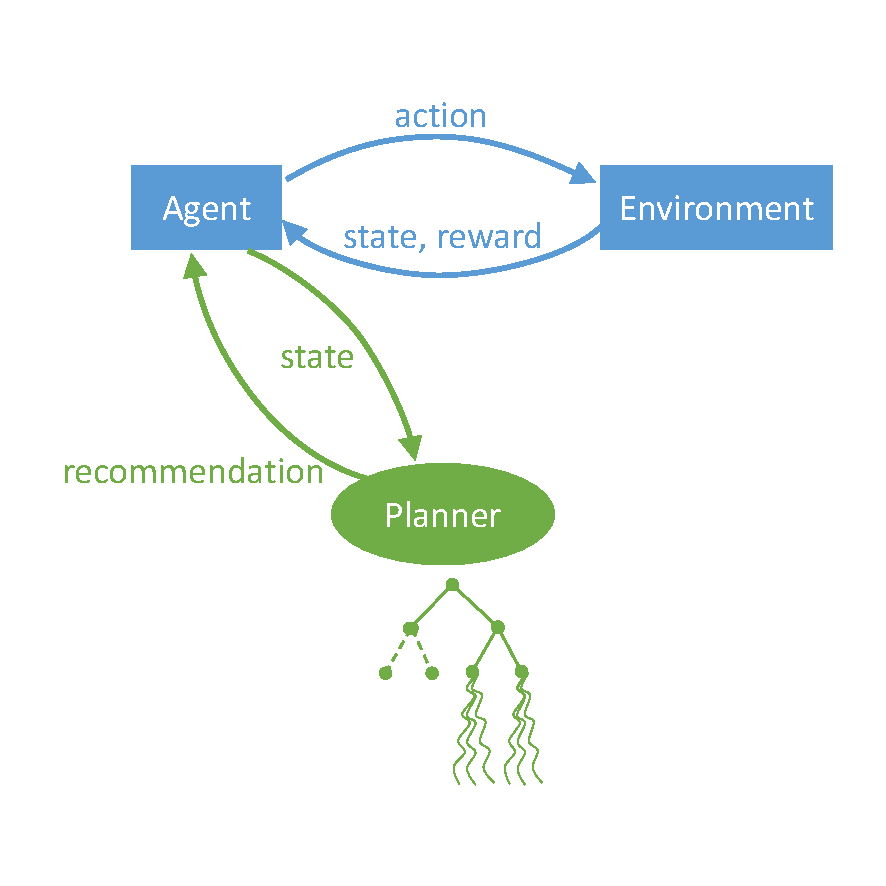
\includegraphics[trim = {0 1.3cm 0 1.3cm}, clip, width=0.7\linewidth]{img/online_planning}
	\caption{Online planning with a generative model. The true interaction cycle between the agent and the environment is depicted \hlb{in blue}. At each step of real interaction, a full planning cycle of simulated trajectories is run, depicted \hlg{in green}.}
	\label{fig:online-planning}
\end{figure}

There are two main frames of analysis for planning algorithms. 
\begin{itemize}
\item In the \emph{fixed-confidence} setting, the generative model is called for a random number of samples $n$ until we can confidently identify an near optimal action:
\begin{equation*}
\probability{\regret(\hat{a}_n) \leq \epsilon} \geq 1-\delta.
\end{equation*}
So-called \gls{PAC} algorithms verifying this property are then evaluated by their expected sample complexity $\expectedvalue [n]$.
\item In the \emph{fixed-budget} setting, the generative model can only be called a fixed number of times $n$. Fixed-budget algorithms aim at minimising the expected simple regret $\expectedvalue[\regret]$.
\end{itemize}
In a real-time scenario, decisions need to be taken at a given frequency, even if this means settling for a suboptimal action. Therefore, we will focus on the fixed-budget setting, whose bounded computational complexity makes it more appropriate for our application.

\gls{MCTS} algorithms were a breakthrough for online decision-making in \glspl{MDP}, that lead to key successes in the domain, including Computer Go \citep{Coulom2006,Silver18}. They enjoy two main benefits: first, they do not require the knowledge of the \gls{MDP} parameters contrary to \textit{e.g.} \gls{DP} algorithms, but only the access to a \emph{generative model} that allows to sample trajectories from the current state. Second, the theoretical performance bounds of \gls{MCTS} algorithms are typically independent of the size of the state space $\cS$. Instead, they depend on the maximum depth at which an optimal node in the search tree can be reached within the allowed budget $n$ of trajectory samples. This translates as an \emph{effective branching factor} in the regret bounds, related to the notion of near-optimality dimension in multi-armed bandits.

\paragraph{Related work}
Algorithms for planning with a generative model date back at least to the seminal work of \citet{Kearns02SS} who proposed the \texttt{Sparse} \texttt{Sampling} algorithm using a tree structure to represent the value estimate and uniform sampling of trajectories. This strategy was further analysed more recently in \citep{Feldman14BRUE}, where the \gls{BRUE} algorithm provides an enhanced value estimation. Another family of algorithms rely on the principle of \gls*{OFU} \citep[surveyed by][]{Munos14}, inspired from the \gls*{MAB} problem. This principle was first used in the context of planning in the \texttt{CrazyStone} software \citep{Coulom2006} for computer Go. It was later formalised with the \gls{UCT} algorithm \citep{Kocsis06UCT}, but was shown by \citet{Coquelin2007} to have a doubly-exponential complexity in the worst case. The \OPD algorithm introduced by \citet{Hren2008optimistic} was the first to provide a polynomial regret bound, but was limited to systems with deterministic rewards and dynamics. It was then extended to stochastic rewards and dynamics with the \glsxtrfull+{OLOP} algorithm \citep{Bubeck2010}, but only in the \emph{open-loop} setting of state-independent policies (\ie sequences of actions), a restriction of the policy class that causes a loss of optimality.
Known stochastic transitions were handled by \citet{Busoniu2012optimistic}. For \glspl{MDP} with stochastic and unknown transitions, polynomial sample complexities have been obtained for \gls{StOP} \citep{Szorenyi14}, \texttt{TrailBlazer} \citep{Grill16} and \texttt{SmoothCruiser} \citep{Grill19}, but despite their theoretical merits these algorithms are intractable in practice: \gls{StOP} requires the expensive storage of policies, while \texttt{TrailBlazer} and \texttt{SmoothCruiser} only terminate after a prohibitive amount of samples, even for very small \glspl{MDP}. %\citep{Huang2017,Kaufmann2017} proposed two algorithms for planning in a maxmin game with stochastic rewards in the leaves of a known game tree.

\paragraph{Contributions} This chapter focuses on two questions. First, in \Cref{sec:olop}, we exhibit a faulty behaviour of the \OLOP algorithm when applied to numerical problems, and propose a modified version that addresses it, leading to an improved performance with a retained guarantee. Second, in \Cref{sec:gbop} we look into how \gls{MCTS} can benefit from merging overlapping trajectories, to better exploit the underlying graphical structure of the dynamics.

\section{Open-loop optimistic planning}
\label{sec:olop}

The goal of this section is two study the empirical performance of the \OLOP algorithm. We focus on that algorithm for its ability to tractably handle stochastic dynamics (though in open-loop only). Indeed, our \gls{MDP} formulation of \Cref{chapter:3} involves unknown parameters in the dynamics, such as the driving styles and destinations of other drivers. Thus, in a probabilistic modelling of this uncertainty, a prior distribution over these unknown parameters induces a distribution over the next state of each observed vehicle, \ie stochastic dynamics. However, \OLOP was introduced with a theoretical sample complexity analysis but no experiment was carried-out. We show that in our experiments this algorithm is overly pessimistic, especially in the low-budget regime, and we provide an intuitive explanation by casting light on an unintended effect that alters its behaviour. We circumvent this issue by leveraging modern tools from the bandits literature to design and analyse a modified version with tighter upper-confidence bounds called \KLOLOP. We show that we retain the asymptotic regret bounds of $\OLOP$ while improving its performances by an order of magnitude in numerical experiments.

This section is structured as follows: in \Cref{sec:kl-olop}, we present \OLOP, give some intuition on its limitations, and introduce \KLOLOP, whose sample complexity is further analysed in \Cref{sec:sample-complexity,sec:regret-proof}, and whose empirical performance is evaluated in \Cref{sec:planning-experiments} in several numerical experiments.

\paragraph{Notations}
We follow the notations from \citep{Bubeck2010} and use the standard notations over alphabets: a finite word $a \in \cA^{\ast}$ of length $h$ represents a sequence of actions $(a_1, \dots, a_h) \in \cA^h$. Its prefix of length $t \leq h$ is denoted $a_{1:t} = (a_1,\dots,a_t) \in \cA^t$. $\cA^\infty$ denotes the set of infinite sequences of actions. Two finite sequences $a\in \cA^{\ast}$ and $b\in \cA^{\ast}$ can be concatenated as $ab\in \cA^{\ast}$, the set of finite and infinite suffixes of $a$ are respectively $a \cA^{\ast} = \{c\in\mathcal{A}^{\star}: \exists b\in \cA^{\ast}$ such that $c=ab\}$ and $a\cA^\infty$ defined likewise, and the empty sequence is $\emptyset$.

During the planning process, the agent iteratively selects sequences of actions until it reaches the allowed budget of $n$ actions. More precisely, at time $t$ during the $m^{\text{th}}$ sequence, the agent played $a^m_{1:t} = a^m_1 \cdots a^m_t \in \cA^t$ and receives a reward $R(s_t^m)$. We denote the probability distribution of this reward as $\nu(a_{1:t}^m) = \probability{R(s_t^m, a_t^m) | s_t^m, a_t^m} \prod_{k=1}^{t-1} \probability{s_{k+1}^m | s_{k}^m, a_{k}^m}$, and its mean as $\mu(a_{1:t}^m)$, where $s_1^m=s_1$ is the current state.


\begin{definition}[Sequence values]
	\begin{leftbar}[defnbar]
	\label{def:sequence-values}
	We define the value $V(a)$ of a sequence of actions $a\in \cA^h$ as the maximum expected discounted cumulative reward one may obtain after executing $a$:
	\begin{equation}
	\label{eq:value}
	V(a) = \sup_{b\in a\cA^\infty} \sum_{t=1}^\infty \discount^t\mu(b_{1:t}).
	\end{equation}
	\end{leftbar}
\end{definition}


\subsection{Kullback-Leibler Open-Loop Optimistic Planning}
\label{sec:kl-olop}

In this section we present \KLOLOP, a combination of the \OLOP algorithm of \citep{Bubeck2010} with the tighter Kullback-Leibler upper confidence bounds from \citep{Cappe2013}. We first frame both algorithms in a common structure before specifying their implementations.

\paragraph{General structure}

First, following \OLOP, the total sample budget $n$ is split in $M$ trajectories of length $L$ in the following way: 
\begin{align*}
&M\text{ is the largest integer such that } M \ceil{\log M/(2 \log 1/\discount)} \leq n;\\
&L= \ceil{\log M / (2 \log 1/\discount)}.
\end{align*}
The look-ahead tree of depth $L$ is denoted $\Tau = \sum_{h=0}^L \cA^h$.

Then, we introduce some useful definitions. Consider episode $1 \leq m \leq M$. For any $1 \leq h \leq L$ and $a\in \cA^h$, let 


\begin{equation*}
N_a(m) \eqdef \sum_{i=1}^m \mathbbm{1}\{a^i_{1:h} = a\}
\end{equation*}


\noindent
be the number of times we played an action sequence starting with $a$, and $S_a(m)$ the sum of rewards collected at the last transition of the sequence $a$
\begin{equation*}
S_a(m) \eqdef \sum_{i=1}^m R(s_h^i, a^i_{1:h}) \mathbbm{1}\{a^i_{1:h} = a\}.
\end{equation*}

\noindent
The empirical mean reward of $a$ is
$\quad\displaystyle{ \hat{\mu}_a(m) \eqdef \frac{S_a(m)}{N_a(m)}} \quad $
if $N_a(m) > 0$, and $+\infty$ otherwise. Here, we provide a more general form for upper and lower confidence bounds on these empirical means:
\begin{align}
\label{eq:u_mu_a_m}
U^{\mu}_a(m) &\eqdef \max \left\{q\in I: N_a(m) d(\hat{\mu}_a(m), q) \leq f(m) \right\}\\
L^{\mu}_a(m) &\eqdef \min \left\{q\in I: N_a(m) d(\hat{\mu}_a(m), q) \leq f(m) \right\}
\end{align}
where $I$ is an interval, $d$ is a divergence on $I\times I \rightarrow \mathbb{R^+}$ and $f$ is a non-decreasing function. They are left unspecified for now and their particular implementations and associated properties will be discussed in the following sections.

These upper-bounds $U^{\mu}_a$ for intermediate rewards finally enable us to define an upper bound $U_a$ for the value $V(a)$ of the entire sequence of actions $a$:
\begin{equation}
\label{eq:Ua}
U_a(m) \eqdef \sum_{t=1}^h \discount^t U^{\mu}_{a_{1:t}}(m) + \frac{\discount^{h+1}}{1-\discount}.
\end{equation}


\noindent
where $\frac{\discount^{h+1}}{1-\discount}$ comes from upper-bounding by one every reward-to-go in the sum \eqref{eq:value}, for $t\geq h+1$. In \citep{Bubeck2010}, there is an extra step to "sharpen the bounds" of sequences $a \in \cA^L$ by taking
\begin{equation}
\label{eq:Ba}
B_a(m) \eqdef \inf_{1 \leq t \leq L} U_{a_{1:t}}(m)
\end{equation}


The general algorithm structure is shown in \Cref{algo:kl-olop}.
We now discuss two specific implementations that differ in their choice of divergence $d$ and non-decreasing function $f$. They are compared in \Cref{tab:comparison}.

\begin{algorithm}[tp]
	\DontPrintSemicolon
	\For{each episode $m = 1, \cdots, M$}{
		Compute $U_a(m-1)$ from \eqref{eq:Ua} for all $a\in\Tau$\;
		Compute $B_a(m-1)$ from \eqref{eq:Ba} for all $a\in \cA^L$\;\label{alg:b_values_compute}
		Sample a sequence with highest B-value: $a^m \in \argmax_{a\in \cA^L} B_a(m-1)$\;
	}
	\Return the most played sequence $a(n) \in \argmax_{a\in \cA^L} N_a(m)$
	\caption{General structure for Open-Loop Optimistic Planning}
	\label{algo:kl-olop}
\end{algorithm}

\begin{table}[tp]
	\caption{Different implementations of \Cref{algo:kl-olop} in \OLOP and \KLOLOP}
	\label{tab:comparison}
	\centering
	\begin{tabular}{ccc}
		\toprule
		Algorithm & \OLOP & \KLOLOP \\
		\midrule
		Interval $I$ & $\mathbb{R}$ & [0, 1] \\
		Divergence $d$ & $\dquad$ & $\dber$ \\
		$f(m)$ & $4 \log M$ & $2\log M + 2 \log\log M$\\
		\bottomrule
	\end{tabular}
\end{table}

\subsubsection{\gls*{OLOP}}
\label{sec:kl-olop-olop}
To recover the original \OLOP algorithm of \citet{Bubeck2010} from \Cref{algo:kl-olop}, we can use a quadratic divergence $\dquad$ on $I=\mathbb{R}$ and a constant function $f_4$ defined as follows:
\begin{equation*}
\dquad(p,q) \eqdef 2(p-q)^2,\qquad
f_4(m) \eqdef 4 \log M
\end{equation*}
Indeed, in this case $U^{\mu}_a(m)$ can then be explicitly computed as
\begin{align*}
U^{\mu}_a(m) &= \max \left\{q\in \mathbb{R}: 2(\hat{\mu}_a(m) - q)^2 \leq \frac{4 \log M }{N_a(m)} \right\} = \hat{\mu}_a(m) + \sqrt{\frac{2 \log M}{N_a(m)}},
\end{align*}
which is the Chernoff-Hoeffding bound used originally in section 3.1 of \citep{Bubeck2010}.

\subsubsection{An unintended behaviour}
\label{sec:kl-olop-behaviour}
From the definition of $U_a(m)$ as an upper-bound of the value of the sequence $a$, we expect increasing sequences $(a_{1:t})_t$ to have non-increasing upper-bounds. Indeed, every new action $a_t$ encountered along the sequence is a potential loss of optimality.
However, this property is only true if the upper-bound defined in \eqref{eq:u_mu_a_m} belongs to the reward interval $[0,1]$.

\begin{lemma}[Monotony of $U_a(m)$ along a sequence]
	\label{lemma:seq_values}
	\begin{leftbar}[lemmabar]
	~\\
	\begin{itemize}
	\item If it holds that $U^{\mu}_b(m) \in [0, 1]$ for all $b\in \cA^{\ast}$, then for any $a\in \cA^L$ the sequence $(U_{a_{1:h}}(m))_{1\leq h \leq L}$ is non-increasing, and we simply have $B_a(m) = U_a(m)$.
	\item Conversely, if $U^{\mu}_b(m) > 1$ for all $b\in \cA^{\ast}$, then for any $a\in \cA^L$ the sequence $(U_{a_{1:h}}(m))_{1\leq h \leq L}$ is non-decreasing, and we have $B_a(m) = U_{a_{1:1}}(m)$.
	\end{itemize}
	\end{leftbar}
\end{lemma}

\begin{proof}
	We prove the first proposition, and the same reasoning applies to the second. For $a\in \cA^L$ and $1 \leq h \leq L - 1$, we have by \eqref{eq:Ua}:
	\begin{align*}
	U_{a_{1:h+1}}(m) - U_{a_{1:h}}(m) &= \discount^{h+1}U^{\mu}_{a_{1:h+1}}(m) + \frac{\discount^{h+2}}{1-\discount} - \frac{\discount^{h+1}}{1-\discount}\\
	&= \discount^{h+1}(\underbrace{U^{\mu}_{a_{1:h+1}}(m)}_{\in [0, 1]} - 1) \leq 0
	%&\leq 0
	\end{align*}
	
	\noindent
	We can conclude that $(U_{a_{1:h}}(m))_{1\leq h \leq L}$ is non-increasing and that $B_a(m) = \inf_{1 \leq h \leq L} U_{a_{1:h}}(m) = U_{a_{1:L}}(m) = U_a(m)$.
\end{proof}

Yet, the Chernoff-Hoeffding bounds used in \OLOP start in the $U^{\mu}_a(m) > 1$ regime -- initially $U^{\mu}_a(m) = \infty$ -- and can remain in this regime for a long time especially in the near-optimal branches where $\hat{\mu}_a(m)$ is close to one.

Under these circumstances, the \Cref{lemma:seq_values} has a drastic effect on the search behaviour. Indeed, as long as a subtree under the root verifies $U^{\mu}_a(m) > 1$ for every sequence $a$, then all these sequences share the same B-value $B_a(m) = U_{a_{1:1}(m)}$. This means that \OLOP cannot differentiate them and exploit information from their shared history as intended, and behaves as uniform sampling instead.
Once the early depths have been explored sufficiently, \OLOP resumes its intended behaviour, but the problem is only shifted to deeper unexplored subtrees.

This consideration motivates us to leverage the recent developments in the Multi-Armed Bandits literature, and modify the upper-confidence bounds for the expected rewards $U^\mu_a(m)$ so that they respect the reward bounds.


\subsubsection{\gls*{KLOLOP}}
\label{sec:kl-olop-kl-olop}

\noindent
We propose a novel implementation of \Cref{algo:kl-olop} where we leverage the analysis of the kl-UCB algorithm from \citep{Cappe2013} for multi-armed bandits with general bounded rewards.
Likewise, we use the Bernoulli Kullback-Leibler divergence defined on the interval $I=[0,1]$ by

\begin{equation*}
\dber(p, q) \eqdef p \log \frac{p}{q} + (1-p)\log\frac{1-p}{1-q}
\end{equation*}

\noindent
with, by convention, $0 \log 0 = 0 \log 0/0 = 0$ and $x \log x /0 = +\infty$ for $x>0$.
This divergence and the corresponding bounds are illustrated in \Cref{fig:ukl}.

\begin{figure}[tp]
	\centering
	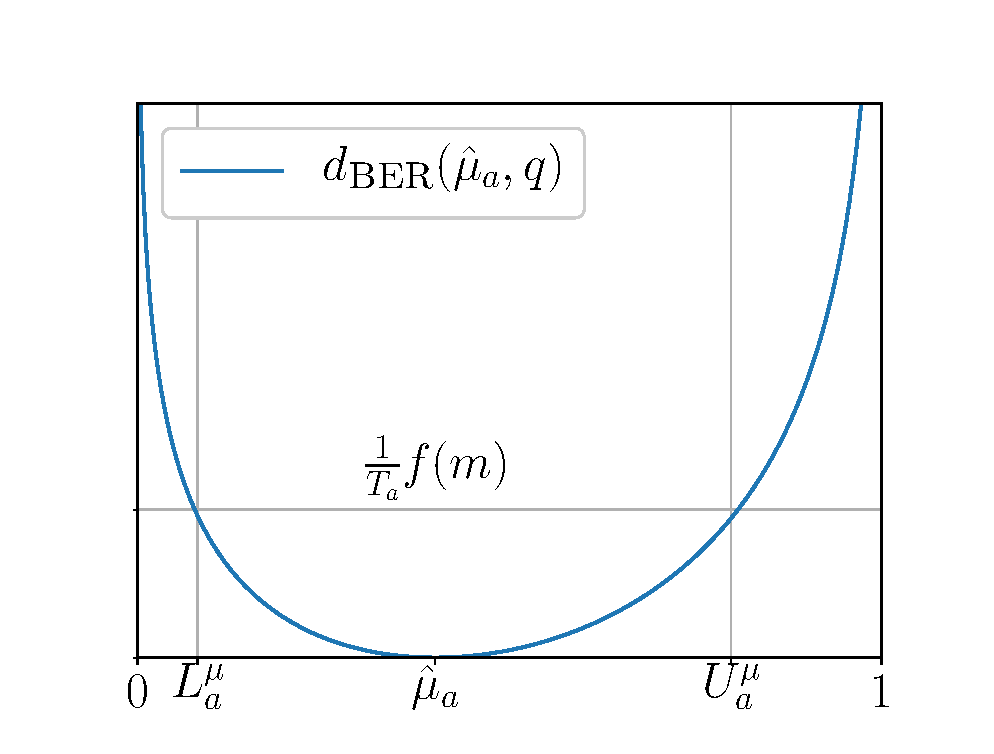
\includegraphics[width=0.6\textwidth]{img/ukl}
	\caption{The Bernoulli Kullback-Leibler divergence $\dber$, and the corresponding upper and lower confidence bounds $U^{\mu}_a$ and $L^{\mu}_a$ for the empirical average $\hat{\mu_a}$. Lower values of $f(m)$ give tighter confidence bounds that hold with lower probabilities.}
	\label{fig:ukl}
\end{figure}

$U^{\mu}_a(m)$ and $L^{\mu}_a(m)$ can be efficiently computed using Newton iterations, as for any $p\in[0, 1]$ the function $q \rightarrow \dber(p,q)$ is strictly convex and increasing (resp. decreasing) on the interval [p, 1] (resp. [0, p]).

Moreover, we use the constant function $f_2: m \rightarrow 2 \log M + 2 \log\log M$. This choice is justified in the end of \Cref{sec:regret-proof}. Because $f_2$ is lower than $f_4$, the \Cref{fig:ukl} shows that the bounds are tighter and hence less conservative than that of \OLOP, which should increase the performance, provided that their associated probability of violation does not invalidate the regret bound of \OLOP.


\begin{remark}[Upper bounds sharpening]
	\label{rmk:sharpen}
	\begin{leftbar}[remarkbar]
	The introduction of the B-values $B_a(m)$ was made necessary in \OLOP by the use of Chernoff-Hoeffding confidence bounds which are not guaranteed to belong to [0, 1]. On the contrary, we have in \KLOLOP that $U^\mu_a(m) \in I = [0,1]$ by construction. By \Cref{lemma:seq_values}, the upper bounds sharpening step in line \ref{alg:b_values_compute} of \Cref{algo:kl-olop} is now superfluous as we trivially have $B_a(m) = U_a(m)$ for all $a\in \cA^L$.
	\end{leftbar}
\end{remark}

\subsection{Sample complexity}
\label{sec:sample-complexity}

We say that $u_n = \tilde{\cO}(v_n)$ if there exist $\alpha, \beta >0$ such that $u_n \leq \alpha \log(v_n)^\beta v_n$.
Let us denote the proportion of near-optimal nodes $\kappa_2$ as


\begin{equation*}
\label{eq:kappa}
\kappa_2 \eqdef \limsup_{h\rightarrow\infty}{\left|\left\{a\in a^H:V(a) \geq V - 2\frac{\discount^{h+1}}{1-\discount}\right\}\right|^{1/h}}
\end{equation*}

\begin{theorem}[Sample complexity]
	\label{thm:regret-kl-olop}
	\begin{leftbar}[theorembar]
	We show that \KLOLOP enjoys the same asymptotic regret bounds as \OLOP. More precisely, for any $\kappa' > \kappa_2$, \KLOLOP satisfies:
	
	
	\begin{equation*}
	\expectedvalue [\regret] = \begin{cases}
	\tilde{\cO}\left(n^{-\frac{\log 1/\discount}{\log \kappa'}}\right) & \text{if}\ \discount\sqrt{\kappa'} > 1; \\
	\tilde{\cO}\left(n^{-\frac{1}{2}}\right) & \text{if}\ \discount\sqrt{\kappa'} \leq 1.
	\end{cases}
	\end{equation*}
	\end{leftbar}
\end{theorem}

We provide a time and memory efficient implementation of \OLOP and \KLOLOP in \Cref{sec:kl-olop-time}, bringing an exponential speedup that allows to scale these algorithms to high sample budgets.

\subsection{Proof of \Cref{thm:regret-kl-olop}}
\label{sec:regret-proof}

We follow step-by step the pyramidal proof of \citep{Bubeck2010}, and adapt it to the Kullback-Leibler upper confidence bound. The adjustments resulting from the change of confidence bounds are \diff{highlighted}. The proofs of lemmas which are not significantly altered are listed in \Cref{sec:kl-olop-proofs}. 

We start by recalling their notations.
Let $1 \leq H \leq L$ and $a^{\star} \in \cA^L$ such that $V(a^{\star}) = V$.
Considering sequences of actions of length $1 \leq h \leq H$, we define the subset $\mathcal{I}_h$ of near-optimal sequences and the subset $\mathcal{J}$ of sub-optimal sequences that were near-optimal at depth $h-1$
\begin{equation*}
\mathcal{I}_h = \left\{a \in \cA^h: V - V(a) \leq 2\frac{\discount^{h+1}}{1-\discount}\right\}, \mathcal{J}_h = \left\{a \in \cA^h: a_{1:h-1} \in \mathcal{I}_{h-1} \text{ and } a \not\in \mathcal{I}_h\right\}
\end{equation*}

By convention, $\mathcal{I}_0 = \{\emptyset\}$. From the definition of $\kappa_2$, we have that for any $\kappa'>\kappa_2$, there exists a constant C such that for any $h \geq 1$,
%\begin{equation*}
$|\mathcal{I}_h| \leq C {\kappa'}^h$
%\end{equation*}
Hence, we also have $|\mathcal{J}_h| \leq K|\mathcal{I}_{h-1}| = O({\kappa'}^h)$.

Now, for $1\leq m \leq M$, $a \in \cA^t$ with $t \leq h$, $h'<h$, we define the set $\mathcal{P}^a_{h,h'}(m)$ of suffixes of $a$ in $\mathcal{J}_h$ that have been played at least a certain number of times
\begin{equation*}
\mathcal{P}^a_{h,h'}(m) = \left\{ b\in a \cA^{h-t}\cap \mathcal{J}_h : N_b(m) \geq \diff{2f(m)}(h+1)^2\discount^{2(h'-h+1)} + 1 \right\}
\end{equation*}

and the random variable

\begin{equation*}
\tau^a_{h,h'}(m) = \mathbbm{1}\{N_a(m-1) < \diff{2f(m)}(h+1)^2\discount^{2(h'-h+1)} + 1 \leq N_a(m)\}
\end{equation*}

\begin{lemma}[Regret and sub-optimal pulls]
	\label{lemma:expected-regret}
	\begin{leftbar}[lemmabar]
	The following holds true:
	\begin{equation*}
	\expectedvalue [\regret] \leq \frac{2K \discount^{H+1}}{1-\discount} +\frac{3K}{M}\sum_{h=1}^H\sum_{a\in\mathcal{J}_h}\frac{\discount^h}{1-\discount}N_a(m)
	\end{equation*}
	\end{leftbar}
\end{lemma}


The rest of the proof is devoted to the analysis of the term $\expectedvalue \sum_{a\in \mathcal{J}_h} N_a(m)$. The next lemma describes under which circumstances a suboptimal sequence of actions in $\mathcal{J}_h$ can be selected.

\begin{lemma}[Conditions for sub-optimal pull]
	\label{lemma:sub-optimal-pull}
	\begin{leftbar}[lemmabar]
	Assume that at step $m+1$ we select a sub-optimal sequence $a^{m+1}$: there exist $0 \leq h \leq L,  a\in \mathcal{J}_h$ such that $a^{m+1} \in a\cA^{\ast}$. Then, it implies that one of the following propositions is true:
	\begin{equation}
	\label{eq:cond-ukl}
	\tag{UCB violation}
	\diff{U_{a^{\star}}(m)} < V,
	\end{equation}
	or
	\begin{equation}
	\tag{LCB violation}
	\label{eq:cond-lkl}
	\sum_{t=1}^h \discount^t \diff{L^{\mu}_{a_{1:t}}(m)} \geq V(a),
	\end{equation}
	or
	\begin{equation}
	\tag{Large CI}
	\label{eq:cond-dkl}
	\sum_{t=1}^h \discount^t\diff{\left(U^{\mu}_{a_{1:t}}(m) - L^{\mu}_{a_{1:t}}(m)\right)} > \frac{\discount^{h+1}}{1-\discount}
	\end{equation}
	\end{leftbar}
\end{lemma}
\begin{proof}
	As $a^{m+1}_{1:h} = a$ and \diff{because the U-values are monotonically increasing along sequences of actions} (see \Cref{rmk:sharpen} and \Cref{lemma:seq_values}), we have $U_a(m) \geq U_{a^{m+1}}(m)$. Moreover, by \Cref{algo:kl-olop}, we have $a^{m+1} = \argmax_{a \in \cA^L}  U_a(m)$ and $a^{\star}\in \cA^L$, so $U_{a^{m+1}}(m) \geq U_{a^{\star}}(m)$ and finally $U_a(m) \geq U_{a^{\star}}(m)$.
	
	Assume that \eqref{eq:cond-ukl} is false, then
	\begin{equation}
	\label{eq:ukl-verifie}
	\sum_{t=1}^h \discount^t U^{\mu}_{a_{1:t}}(m) + \frac{\discount^{h+1}}{1-\discount} = U_a(m) \geq U_{a^{\star}}(m) \geq V
	\end{equation}
	Assume that \eqref{eq:cond-lkl} is false, then
	\begin{equation}
	\label{eq:lkl-verifie}
	\sum_{t=1}^h \discount^t L^{\mu}_{a_{1:t}}(m) < V(a),
	\end{equation}
	By taking the difference \eqref{eq:ukl-verifie} - \eqref{eq:lkl-verifie}, 
	\begin{equation*}
	\sum_{t=1}^h \discount^t \left(U^{\mu}_{a_{1:t}}(m) - L^{\mu}_{a_{1:t}}(m)\right) + \frac{\discount^{h+1}}{1-\discount} > V - V(a)
	\end{equation*}
	But $a \in \mathcal{J}_h$, so $V - V(a) \geq \frac{2\discount^{h+1}}{1-\discount}$, which yields \eqref{eq:cond-dkl} and concludes the proof.
\end{proof}

\diff{In the following lemma, for each episode $m$ we bound the probability of \eqref{eq:cond-ukl} or \eqref{eq:cond-lkl} by a desired confidence level $\delta_m$, whose choice we postpone until the end of this proof. For now, we simply assume that we picked a function $f$ that satisfies $f(m)\log (m) e^{-f(m)} = O(\delta_m)$. We also denote $\Delta_M = \sum_{m=1}^{M}\delta_m$.}

\begin{lemma}[Boundary crossing probability]
	\label{lemma:boundary-crossing-prob}
	\begin{leftbar}[lemmabar]
	The following holds true, for any $1 \leq h \leq L$ and $m \leq M$,
	\begin{equation*}
	\probability{\text{\eqref{eq:cond-ukl} or \eqref{eq:cond-lkl} is true}} = \diff{O((L+h)\delta_m)}
	\end{equation*}
	\end{leftbar}
\end{lemma}
\begin{proof}
	Since $V \leq \sum_{t=1}^h \discount^t \mu(a^{\star}_{1:t}) + \frac{\discount^{h+1}}{1-\discount}$, we have,
	\begin{align*}
	\probability{\eqref{eq:cond-ukl}} &=  \probability{U_{a^{\star}}(m) \leq V}\\
	&= \probability{\sum_{t=1}^L \discount^t U^{\mu}_{a^{\star}_{1:t}}(m) \leq \sum_{t=1}^L \discount^t \mu(a^{\star}_{1:t})}\\
	&\leq \probability{\exists 1\leq t \leq L : U^{\mu}_{a^{\star}_{1:t}}(m) \leq \mu(a^{\star}_{1:t})} \\
	&\leq \sum_{t=1}^L\probability{U^{\mu}_{a^{\star}_{1:t}}(m) \leq \mu(a^{\star}_{1:t})}
	\end{align*}
	
	\diff{In order to bound this quantity, we reduce the question to the application of a deviation inequality. For all $1\leq t\leq L$, we have on the event $\{U^{\mu}_{a^{\star}_{1:t}}(m) \leq \mu(a^{\star}_{1:t})\}$ that $\hat{\mu}_{a^{\star}_{1:t}}(m) \leq U^{\mu}_{a^{\star}_{1:t}}(m) \leq \mu(a^{\star}_{1:t}) < 1$. Therefore, for all $0 < \delta < 1 - \mu(a^{\star}_{1:t})$, by definition of $U^{\mu}_{a^{\star}_{1:t}}(m)$:}
	
	\begin{equation*}
	\diff{d(\hat{\mu}_{a^{\star}_{1:t}}(m), U^{\mu}_{a^{\star}_{1:t}}(m)+\delta) > \frac{f(m)}{N_{a^{\star}_{1:t}}(m)}}
	\end{equation*}
	
	\diff{As $d$ is continuous on $(0,1)\times[0, 1]$, we have by letting $\delta \rightarrow 0$ that:}
	
	\begin{equation*}
	\diff{d(\hat{\mu}_{a^{\star}_{1:t}}(m), U^{\mu}_{a^{\star}_{1:t}}(m)) \geq \frac{f(m)}{N_{a^{\star}_{1:t}}(m)}}
	\end{equation*}
	
	\diff{Since d is non-decreasing on $[\hat{\mu}_{a^{\star}_{1:t}}(m), \mu(a^{\star}_{1:t})]$,}
	
	\begin{equation*}
	\diff{d(\hat{\mu}_{a^{\star}_{1:t}}(m), \mu(a^{\star}_{1:t})) \geq d(\hat{\mu}_{a^{\star}_{1:t}}(m), U^{\mu}_{a^{\star}_{1:t}}(m)) \geq \frac{f(m)}{N_{a^{\star}_{1:t}}(m)}}
	\end{equation*}
	
	\diff{We have thus shown the following inclusion:}
	
	\begin{equation*}
	\diff{\{U^{\mu}_{a^{\star}_{1:t}}(m) \leq \mu(a^{\star}_{1:t})\} \subseteq \left\{ \mu(a^{\star}_{1:t}) > \hat{\mu}_{a^{\star}_{1:t}}(m) \text{ and } d(\hat{\mu}_{a^{\star}_{1:t}}(m), \mu(a^{\star}_{1:t})) \geq \frac{f(m)}{N_{a^{\star}_{1:t}}(m)} \right\}}
	\end{equation*}
	
	\diff{Decomposing according to the values of $N_{a^{\star}_{1:t}}(m)$ yields:}
	
	\begin{equation*}
	\diff{\{U^{\mu}_{a^{\star}_{1:t}}(m) \leq \mu(a^{\star}_{1:t})\} \subseteq \bigcup_{n=1}^m \left\{ \mu(a^{\star}_{1:t}) > \hat{\mu}_{a^{\star}_{1:t}, n} \text{ and } d(\hat{\mu}_{a^{\star}_{1:t}, n}, \mu(a^{\star}_{1:t})) \geq \frac{f(m)}{n} \right\}}
	\end{equation*}
	
	\diff{We now apply the deviation inequality provided in Lemma 2 of Appendix A in \citep{Cappe2013}: $\forall \epsilon > 1$, provided that $0 < \mu(a^{\star}_{1:t}) < 1$,}
	
	\begin{equation*}
	\diff{\probability{\bigcup_{n=1}^m \left\{ \mu(a^{\star}_{1:t}) > \hat{\mu}_{a^{\star}_{1:t}, n} \text{ and } n \dber(\hat{\mu}_{a^{\star}_{1:t}, n}, \mu(a^{\star}_{1:t})) \geq \epsilon \right\}} \leq e\ceil{\epsilon \log m}e^{-\epsilon}\,.}
	\end{equation*}
	
	\diff{By choosing $\epsilon = f(m)$, it comes}
	\begin{align*}
	\diff{\probability{\eqref{eq:cond-ukl}} \leq \sum_{t=1}^L e\ceil{f(m)\log m}e^{-f(m)} = O(L\delta_m)}
	\end{align*}
	
	The same reasoning gives: $\quad\displaystyle{
		\probability{\eqref{eq:cond-lkl}} = \diff{O(h\delta_m)}}$.
\end{proof}

\begin{lemma}[Confidence interval length and number of plays]
	\label{lemma:ci-length}
	\begin{leftbar}[lemmabar]
	Let $1 \leq h \leq L$, $a\in \mathcal{J}_h$ and $0 \leq h' < h$. Then  \eqref{eq:cond-dkl} is not satisfied if the following propositions are true:
	\begin{equation}
	\label{eq:sampled-enough-h}
	\forall 0\leq t\leq h', N_{a_{1:t}}(m) \geq \diff{2f(m)}(h+1)^2\discount^{2(t-h-1)}
	\end{equation}
	and
	\begin{equation}
	\label{eq:sampled-enough}
	N_{a}(m) \geq \diff{2f(m)}(h+1)^2\discount^{2(h'-h-1)}
	\end{equation}
	\end{leftbar}
\end{lemma}
\begin{proof}
	We start by providing an explicit upper-bound for the length of the confidence interval $U^{\mu}_{a_{1:t}} - L^{\mu}_{a_{1:t}}$. \diff{By Pinsker's inequality:}
	
	\begin{equation*}
	\diff{\dber(p, q) > \dquad(p, q)}
	\end{equation*}
	
	\diff{Hence for all $C>0$, }
	\begin{equation*}
	\diff{\dber(p, q) \leq C   \implies 2(q - p)^2 < C  \implies p - \sqrt{C/2} < q < p + \sqrt{C/2}}
	\end{equation*}
	\diff{And thus, for all $b\in \cA^{\ast}$, by definition of $U^{\mu}$ and $L^{\mu}$:}
	\begin{align*}
	\diff{U^{\mu}_{b}(m) - L^{\mu}_{b}(m) \leq \frac{S_b(m)}{N_b(m)} + \sqrt{\frac{f(m)}{2N_b(m)}} -  \left(\frac{S_b(m)}{N_b(m)} - \sqrt{\frac{f(m)}{2N_b(m)}}\right) 
		= \sqrt{\frac{2f(m)}{N_b(m)}}}
	\end{align*}
	
	Now, assume that \eqref{eq:sampled-enough-h} and \eqref{eq:sampled-enough} are true. Then, we clearly have
	\begin{align*}
	\sum_{t=1}^h \discount^t\left(U^{\mu}_{a_{1:t}}(m) - L^{\mu}_{a_{1:t}}(m)\right) &\leq \sum_{t=1}^{h'} \discount^t \sqrt{\frac{2f(m)}{N_{a_{1:t}}(m)}} + \sum_{t=h'+1}^h \discount^t \sqrt{\frac{2f(m)}{N_{a_{1:t}}(m)}} \\
	&\leq \frac{1}{(h+1)\discount^{-h-1}} \sum_{t=1}^{h'} 1 + \frac{1}{(h+1)\discount^{-h-1}} \sum_{t=h'+1}^h \discount^{t-h'}  \\
	&\leq \frac{\discount^{h+1}}{h+1} \left( h' + \frac{\discount}{1-\discount} \right)\leq \frac{\discount^{h+1}}{1-\discount}\,.
	\end{align*}
\end{proof}

\begin{lemma}
	\label{lemma:size_Ph}
	\begin{leftbar}[lemmabar]
	Let $1 \leq h \leq L,  a\in \mathcal{J}_h$ and $0\leq h'<h$. Then $\tau^a_{h,h'}=1$ implies that either equation \eqref{eq:cond-ukl} or \eqref{eq:cond-lkl} is satisfied or the following proposition is true:
	
	
	\begin{equation}
	\label{eq:P-min-size}
	\exists 1\leq t \leq h': |\mathcal{P}_{h,h'}^{a_{1:t}}(m)| < \discount^{2(t-h')}
	\end{equation}
	\end{leftbar}
\end{lemma}

\begin{lemma}
	\label{lemma:expected-P-size}
    \begin{leftbar}[lemmabar]
	Let $1\leq h\leq L$ and $0 \leq h' < h$. Then the following holds true,
	
	\begin{equation*}
	\expectedvalue |\mathcal{P}^\emptyset_{h,h'}(M)| = \tilde{O}\left(\discount^{-2h'}\mathbbm{1}_{h'>0}\sum_{t=0}^{h'}(\discount^2 \kappa')^t + (\kappa')^h\diff{\Delta_M} \right).
	\end{equation*}
	\end{leftbar}
\end{lemma}

\begin{lemma}
	\label{lemma:expected-plays-count}
	\begin{leftbar}[lemmabar]
	Let $1\leq h\leq L$. The following holds true,
	\begin{equation*}
	\expectedvalue \sum_{a\in \mathcal{J}_h} N_a(m) = \tilde{O}\left(\discount^{-2h} + \diff{(\kappa')^h(1+M\Delta_M+\Delta_M) + (\kappa'\discount^{-2})^h\Delta_M}\right)
	\end{equation*}
	\end{leftbar}
\end{lemma}

Thus by combining \Cref{lemma:expected-regret,lemma:expected-plays-count} we obtain
\begin{equation*}
\expectedvalue [\regret] = \tilde{O}\left(\discount^H + \discount^{-H}M^{-1} + (\kappa' \discount)^{H}M^{-1}\diff{(1+M\Delta_M+\Delta_M)} + (\kappa')^H\discount^{-H}M^{-1}\diff{\Delta_M}\right)
\end{equation*}
Finally,
\begin{itemize}
	\item if $\kappa'\discount^2 \leq 1$, we take $H = \floor{\log M / (2\log 1/\discount)}$ to obtain
	\begin{equation*}
	\expectedvalue [\regret] = \tilde{O}\left(M^{-\frac{1}{2}} + M^{-\frac{1}{2}} + M^{-\frac{1}{2}}M^{\frac{\log \kappa'}{2\log 1/\discount}} \diff{\Delta_M}\right)
	\end{equation*}
	For the last term to be of the same order of the others, we need to have $\Delta_M = O(M^{-\frac{\log \kappa'}{2\log 1/\discount}})$. Since $\kappa'\discount^2 \leq 1$, we achieve this by taking \diff{$\Delta_M = O(M^{-1})$}.
	\item if $\kappa'\discount^2 > 1$, we take $H = \floor{\log M / \log \kappa'}$ to obtain
	\begin{equation*}
	\expectedvalue [\regret] = \tilde{O}\left(M^{\frac{\log \discount}{\log \kappa'}} + M^{\frac{\log \discount}{\log \kappa'}}\diff{(1+M\Delta_M+\Delta_M)} + M^{\frac{\log 1/\discount}{\log \kappa'}}\diff{\Delta_M}\right)
	\end{equation*}
	Since $\kappa'\discount^2 > 1$, the dominant term in this sum is $M^{\frac{\log \discount}{\log \kappa'}}M\Delta_M$. Again, taking \diff{$\Delta_M = O(M^{-1})$} yields the claimed bounds.
\end{itemize}
Thus, the claimed bounds are obtained in both cases as long as we can impose $\Delta_M = O(M^{-1})$, that is, find a sequence $(\delta_m)_{1\leq m\leq M}$ and a function $f$ verifying:
\begin{equation}
\sum_{m=1}^M \delta_m = O(M^{-1})\quad \text{and}\quad f(m)\log (m) e^{-f(m)} = O(\delta_m)
\end{equation}

By choosing \diff{$\delta_m = M^{-2}$ and $f(m) = 2 \log M + 2 \log\log M$}, the corresponding \KLOLOP algorithm does achieve the regret bound claimed in \Cref{thm:regret-kl-olop}.


\subsection{Experiments}
\label{sec:planning-experiments}

We have performed some numerical experiments to evaluate and compare the following planning algorithms\footnote[1]{The source code is available at \url{https://eleurent.github.io/kl-olop/}}:
\begin{itemize}
	\item \texttt{Random}: returns a random action, we use it as a minimal performance baseline.
	\item \OPD: the \emph{Optimistic Planning for Deterministic systems} from \citep{Hren2008}, used as a baseline of optimal performance. This planner is only suited for deterministic environments, and exploits this property to obtain faster rates. However, it is expected to fail in stochastic environments.
	\item \OLOP: as described in \Cref{sec:kl-olop-olop}.\footnote[2]{Note that we use the lazy version of $\OLOP$ and $\KLOLOP$ presented in \Cref{sec:kl-olop-time}, otherwise the exponential running-time would have been prohibitive.}
	\item \KLOLOP: as described in \Cref{sec:kl-olop-kl-olop}.\footnotemark[2]
	\item \KLOLOP(1): an aggressive version of \KLOLOP where we used $f_1(m) = \log M$ instead of $f_2(m)$. This threshold function makes the upper bounds even tighter, at the cost of an increased probability of violation. Hence, we expect this solution to be more efficient in close-to-deterministic environments. However, since we have no theoretical guarantee concerning its regret as we do with $\KLOLOP$, it might not be conservative enough and converge too early to a suboptimal sequence, especially in highly stochastic environments.
\end{itemize}
%TODO: probleme de reference des sous-sections dans le itemize.

They are evaluated on the following tasks, using a discount factor of $\discount=0.8$:
\begin{itemize}
	\item A \href{https://github.com/eleurent/highway-env/}{highway driving} environment \citep{highway-env}: a vehicle is driving on a road randomly populated with other slower drivers, and must make their way as fast as possible while avoiding collisions by choosing on the the following actions: \texttt{change-lane-left}, \texttt{change-lane-right}, \texttt{no-op}, \texttt{faster}, \texttt{slower}.
	\item A \href{https://github.com/maximecb/gym-minigrid}{gridworld} environment \citep{gym_minigrid}: the agent navigates in a randomly-generated gridworld composed of either empty cells, terminal lava cells, and goal cells where a reward of $1$ is collected at the first visit.
	\item A stochastic version of the gridworld environment with noisy rewards, where the noise is modelled as a Bernoulli distribution with a 15\% probability of error, i.e. receiving a reward of 1 in an empty cell or 0 in a goal cell.
\end{itemize}

\begin{figure}[pth]
	\centering
	\begin{subfigure}[b]{0.8\linewidth}
		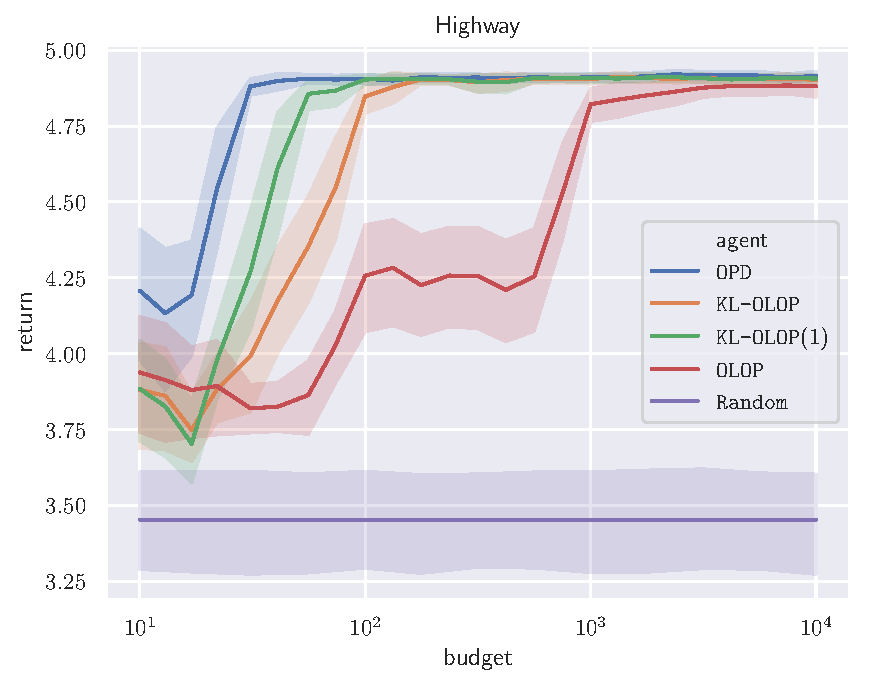
\includegraphics[width=\textwidth]{img/hw_return_svg-tex}
		\caption{Highway}
		\label{sub:highway}
	\end{subfigure}
	\newline
	\begin{subfigure}[b]{0.49\linewidth}
		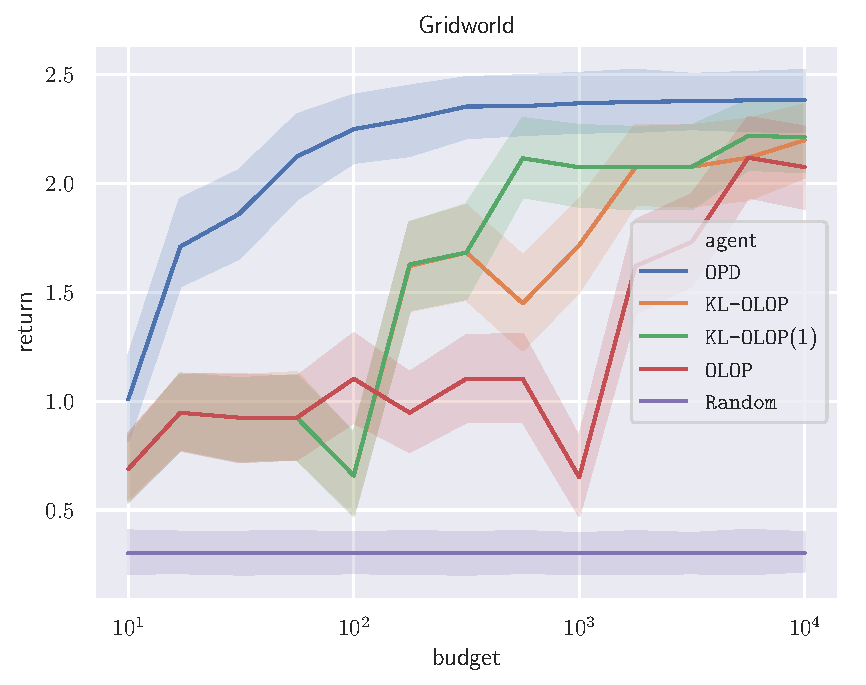
\includegraphics[width=\textwidth]{img/gw_return_svg-tex}
		\caption{Gridworld}
		\label{sub:gridworld}
	\end{subfigure}
	\begin{subfigure}[b]{0.49\linewidth}
		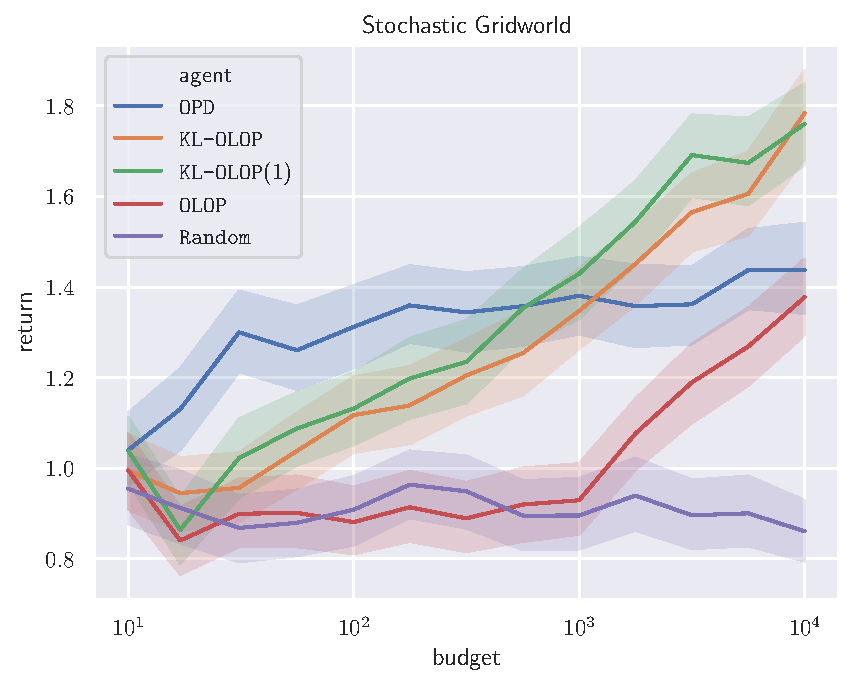
\includegraphics[width=\textwidth]{img/gw_stoch_return_svg-tex}
		\caption{Stochastic Gridworld}
		\label{sub:gridworld_stoch}
	\end{subfigure}
	\caption{Numerical experiments: for each environment-agent configuration, we compute the average return over 100 runs –- along with its 95\% confidence interval –- with respect to the available budget $n$.}
	\label{fig:experiments}
\end{figure}

\begin{figure}[pth]
	\centering
	
	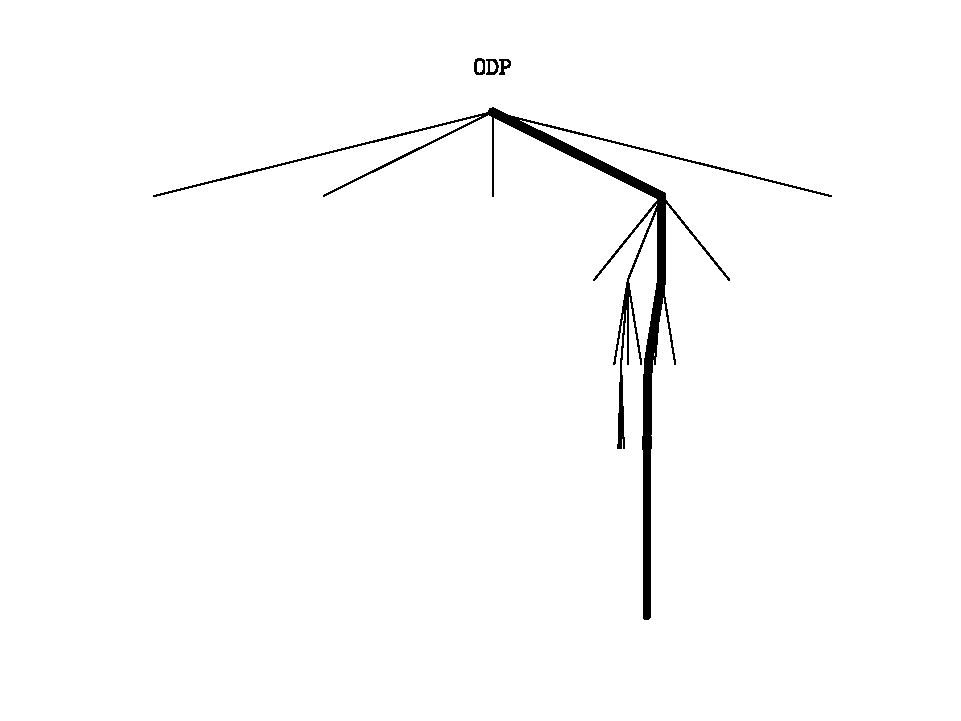
\includegraphics[width=0.6\textwidth]{img/tree_OPD_svg-tex} 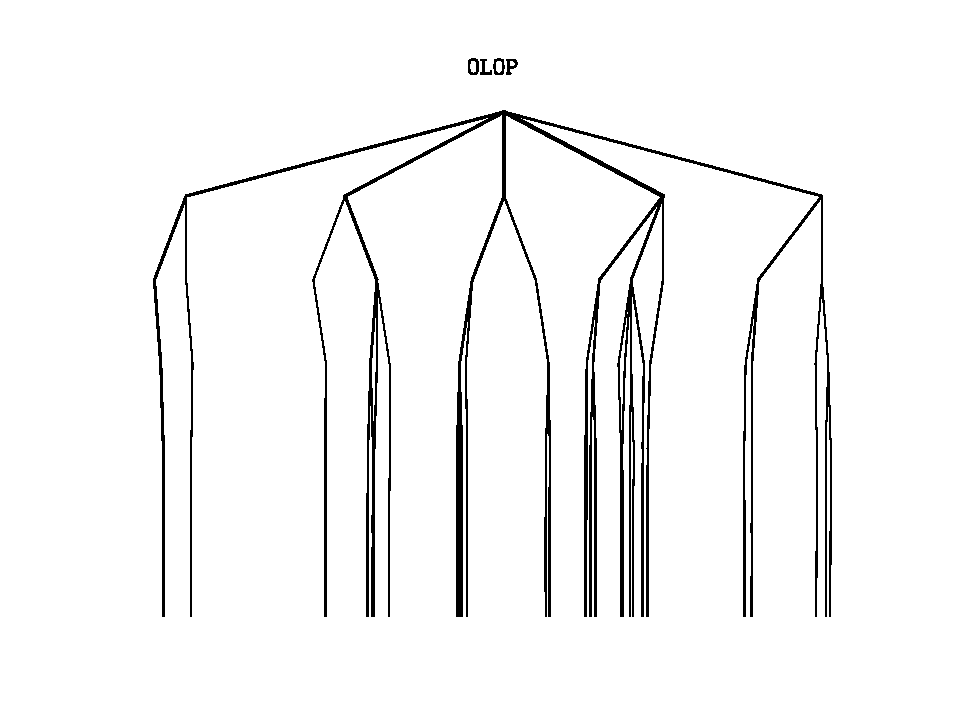
\includegraphics[width=0.6\textwidth]{img/tree_OLOP_svg-tex}
	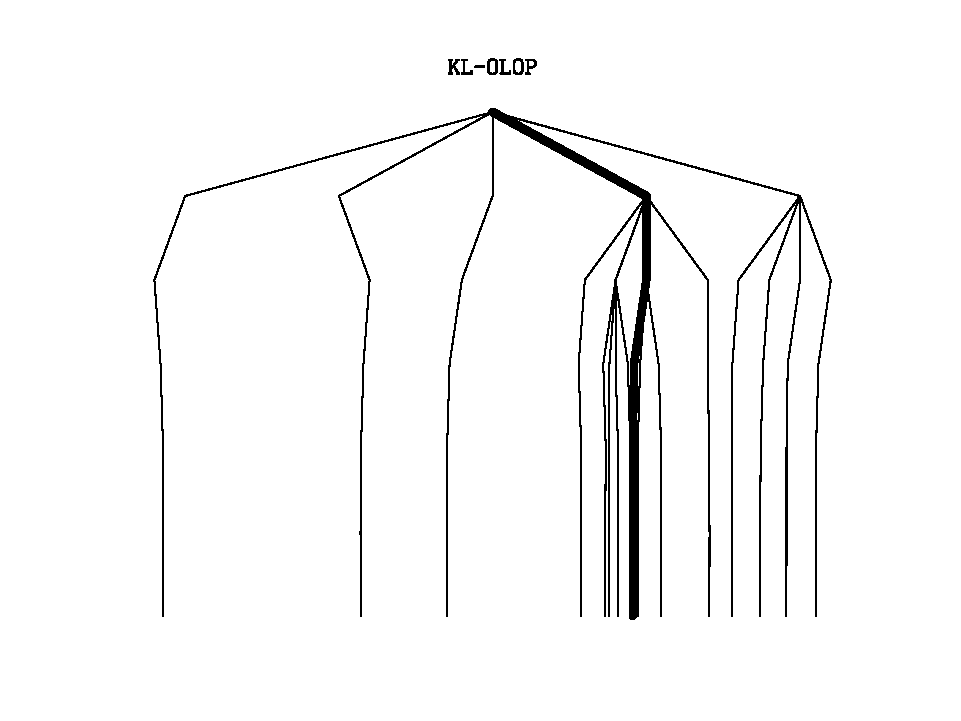
\includegraphics[width=0.6\textwidth]{img/tree_KL-OLOP_svg-tex}
	
	\caption{The look-ahead trees (down to depth 6) expanded by the planning algorithms from the same initial state in the highway environment with the same budget $n=10^3$. The width of edges represents the nodes visit count $N_a(m)$.}
	\label{fig:trees}
\end{figure}

The results of our experiments are shown in \Cref{fig:experiments}. The \OPD algorithm converges very quickly to the optimal return in the two first environments, shown in \Cref{sub:highway} and \Cref{sub:gridworld}, because it exploits their deterministic nature: it needs neither to estimate the rewards through upper-confidence bounds nor to sample whole sequences all the way from the root when expanding a leaf, which provides a significant speed-up. It can be seen as an oracle allowing to measure the conservativeness of stochastic planning algorithms. And indeed, even before introducing stochasticity, we can see that \OLOP performs quite badly on the two environments, only managing to solve them with a budget in the order of $10^{3.5}$. In stark contrast, \KLOLOP makes a much better use of its samples and reaches the same performance an order of magnitude faster. This is illustrated by the expanded trees shown in \Cref{fig:trees}: \OPD exploits the deterministic setting and produces a sparse tree densely concentrated around the optimal trajectory. Conversely, the tree developed by \OLOP is evenly balanced, which suggests that \OLOP behaves as uniform planning as hypothesised in \Cref{sec:kl-olop-behaviour}. \KLOLOP is more efficient and expands a highly unbalanced tree, exploring the same regions as \OPD. Furthermore, in the stochastic gridworld environment shown in \Cref{sub:gridworld_stoch}, we observe that the deterministic \OPD planner's performance saturates as it settles to suboptimal trajectories, as expected. Conversely, the stochastic planners all find better-performing open-loop policies, which justifies the need for this framework. Again, \KLOLOP converges an order of magnitude faster than \OLOP. Finally, \KLOLOP(1) enjoys good performance overall and displays the most satisfying trade-off between aggressiveness in deterministic environments and conservativeness in stochastic environments; hence we recommend this tuning for practical use.

\subsection{On a closed-loop algorithm}

We briefly mention an extension of \KLOLOP to closed-loop policies, in the setting where the transitions have a finite support of size $B < \infty$. The algorithm, named \MDPGapE, was developed as part of a collaboration \citep{Jonsson2020planning} and analysed in the fixed-confidence setting.

It relies on estimating confidence sets $\cC_t$ on the probability vector $p(\cdot|s,a)$
$$\cC_t(s,a) \eqdef \left\{p\in \Sigma_S :  \KL\!\big(\hp_t(\cdot|s,a),p\big) \leq \frac {\beta^p(n_t(s,a), n)} {n_t(s,a)}\right\},$$

and forming recursive upper and lower confidence bounds in the form
\begin{align*}
U_{h}(s) &= \max_{a\in \cA} \left[u_t(s,a) + \discount \max_{q \in \cC_t(s,a)} \sum_{s'} q(s'|s,a) U_{h+1}(s')\right], \\
L_{h}(s) &= \max_{a\in \cA} \left[\ell_t(s,a) + \discount \min_{q \in \cC_t(s,a)} \sum_{s'} q(s'|s,a)L_{h+1}(s')\right].
\end{align*}

\section{Graph-based optimistic planning}
\label{sec:gbop}


The goal of this section is to address a limitation of \gls{MCTS} algorithms: they rely on a tree structure that  --despite its simplicity-- \emph{does not allow to merge information across states}. That is, if a state $s$ can be reached via two trajectories, it will be represented twice in the look-ahead tree. For instance, in \Cref{fig:structures} (left), two paths lead to the same state represented in orange. \gls{MCTS} algorithms do not merge the information of the two trajectories to update a shared estimate of the state value.

\paragraph{Related work}

The idea of merging information between branches of a search tree appears in \citep{Silver18}, where the state values are approximated with a shared Neural Network. However, this network is merely updated between two planning instances and not during the planning procedure itself.
Another work of interest is that of \citet{Hostetler14}, who propose to partition the state space $S$ into a smaller set $\cY$ of equivalence classes. By aggregating similar states within a class, they reduce the branching factor of the search tree from $|\cS||\cA|$ to $|\cY||\cA|$, which substantially improves sample complexity as they illustrate empirically. However, this procedure requires providing a relevant state partition, only aggregates trajectories that traverse the same sequence of classes (\emph{i.e.} local deformations), and comes with a (bounded) loss of optimality.
The closest work to ours is that of \citet{Ballesteros2013}, in the context of partially observable \glspl{MDP}, who identify similar belief states and plan with a graph structure. This work focuses on empirically comparing various similarity measures on robotic tasks and does not provide any theoretical analysis of the effect of aggregation. This is precisely our goal and contribution here.

In this section, we introduce a planning algorithm named \GBOPD, a graph-based version of the tree-based \OPD algorithm for deterministic systems. We analyse the benefits of this graph-based formulation in \Cref{sec:gbop-analysis}, and provide in \Cref{thm:regret-gbop} a regret guarantee. The corresponding regret bound features a novel problem-dependent difficulty measure that we introduce to capture the benefit of using a graph structure. We show that this measure can only improve over the performance of \OPD, and provide an example where it does. We discuss in \Cref{sec:gbop-stochastic} an extension of our method to stochastic MDPs, called \GBOP. Finally, \Cref{sec:gbop-experiments} illustrates the benefits of \GBOP in two numerical simulations.

\subsection{Graph-Based Planning for Deterministic Systems}
\label{sec:gbopd}

In this section, we introduce a simple yet highly effective variant of tree-based planning algorithms. We first consider the simple setting of \glspl{MDP} with deterministic dynamics, and will denote $P(s,a)$ the unique next state $s'$ sampled from $P\left(s'|s,a\right)$.
We start by giving some background on the interplay of data structures and optimistic planning algorithms.

\subsubsection{Data structures}

In this work, we compare two data structures for planning in an MDP: tree and (directed) graph, represented in \Cref{fig:structures}. In order to distinguish them, we referring to trees with Roman symbols, e.g. $T, U, L, B$; and to graphs with calligraphic symbols, e.g. $\cG, \cU, \cL, \cB$. In both structures, we say that a node is \emph{internal} if it has outgoing edges, and \emph{external} else.

\begin{figure}[tp]
	\centering
	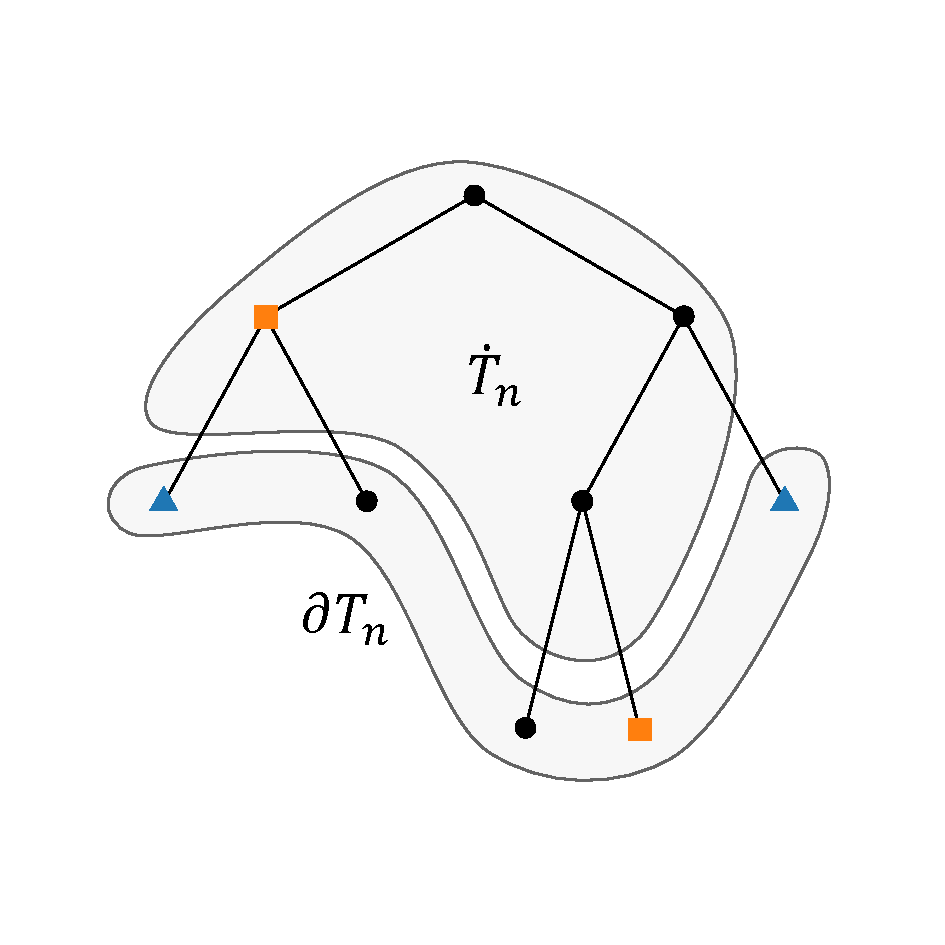
\includegraphics[trim={1.8cm 2.2cm 1.9cm 2.7cm}, clip,width=0.46\linewidth]{img/gbop/tree_1}
	\hfill
	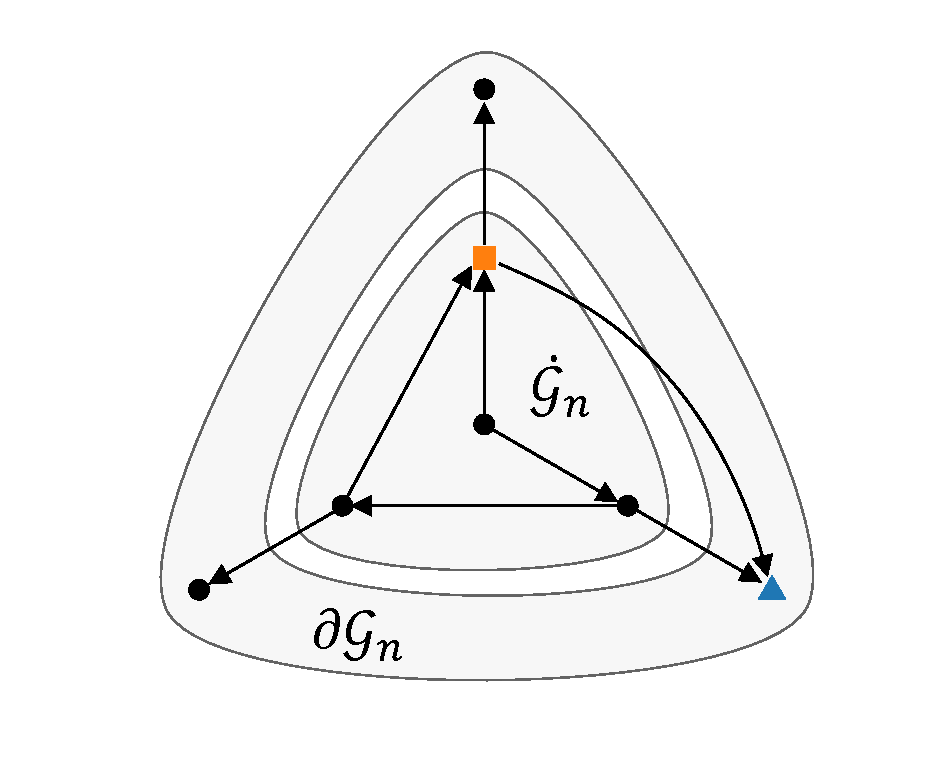
\includegraphics[trim={1.8cm 1.2cm 1.9cm 0.8cm}, clip,width=0.46\linewidth]{img/gbop/graph_1}
	\caption{Illustration of the tree $\Tau_n$ (left) and the graph $\cG_n$ (right) built from the same observed transitions. The root of the tree corresponds to the central graph node. In the tree, two nodes with the same colour and shape (not black round) lead to the same state.}
	\label{fig:structures}
\end{figure}

In a tree, a node of depth $h$ represents a sequence of actions $a\in \cA^h$. The \emph{root} of the tree corresponds to the empty action sequence, and hence to the initial state $s_1\in S$. At iteration $n$, we denote the current tree as $\Tau_n$. Borrowing notations from topology, we denote its set of internal nodes as $\inte{\Tau}_n$ and its set of external nodes (the leaves) as $\ext{\Tau}_n$. Note that since the \gls{MDP} is deterministic, a sequence of action $a$ is associated with its final state denoted $s(a)$, but this association is not one-to-one: several sequences of action can lead to the same state, which will be represented several times in the tree.

In a graph, the nodes represent states $s\in S$, and the edges represent transitions between states. The \textit{source} of the graph corresponds to the initial state $s_0$. At iteration $n$, we denote the current graph as $\cG_n$, its set of internal nodes as $\inte{\cG}_n$ and its set of \textit{sinks} as $\ext{\cG}_n$.

Both structures are built iteratively from a single starting node, by selecting an external node (leaf or sink) to expand. The \emph{expansion} of a node $a$ or $s$ refers to calling the generative model to sample the reward $r$ and next state $s'$ for each action $a\in \cA$, and adding child nodes to the data structure. In a tree, the expansion of a node $a\in \cA^h$ always lead to the creation of new leaves that represent the suffix sequence of action $ab\in \cA^{h+1},\, b\in \cA$. The maximum depth of an expanded node in $T_n$ is denoted $d_n$. In contrast, in a graph the next state $s'$ reached from $s,a$ might already be present in $\cG_n$, in which case we add the edge between $s$ and $s'$ without creating a new node.
These data structures can be used to store information about the \gls{MDP}, such as the transitions and rewards $r(s, a)$, or other informations useful for planning.

% TODO: n->m is the number of expansions, not the number of samples n. ie n = m|A|.


\subsubsection{Optimistic planning}

A planning algorithm is typically composed of two main rules:
\begin{enumerate}[label=(\roman*)]
	\item A \emph{sampling rule}, that selects promising transitions to simulate at each iteration $n$;
	\item A \emph{recommendation rule}, that recommends a good first action $\hat{a}_n$ to take (in $s_1$).
\end{enumerate}

These rules can be chosen with the goal of minimising the simple regret $\regret$.
A popular approach is to follow the principle of \glsxtrfull{OFU} \citep[see][]{Munos14}, which consists in exploring the option that maximises an upper-bound of the true objective. In the context of planning, it has been applied by forming bounds on the state value function $\V^\star$, that we simply denote $\V$ for brevity.

\begin{definition}[Value bounds]
	\begin{leftbar}[defnbar]
	{\textbf{On trees.}} We denote by $L:\Tau_n \rightarrow \Real$ and  $U:\Tau_n \rightarrow \Real$ a lower-bound and upper-bound for the state value $V$ defined on the tree $\Tau_n$, such that
	\begin{equation*}
	\forall a\in\Tau_n, \qquad L(a) \leq V(s(a)) \leq U(a).
	\end{equation*}
	
	{\textbf{On graphs.}} Likewise, we denote by $\cL:\cG_n \rightarrow \Real$ and  $\cU:\cG_n \rightarrow \Real$ a lower-bound and upper-bound for the state value $V$ defined on the graph $\cG_n$, such that
	\begin{equation*}
	\forall s\in\cG_n, \qquad \cL(s) \leq V(s) \leq \cU(s).
	\end{equation*}
	\end{leftbar}
\end{definition}

Following the \gls{OFU} principle, at iteration $n$ we must leverage available information to design an upper-bound $U_n$ (or $\cU_n$) on $V$ as tight as possible. Then, in order to select a promising external node to expand, the sampling rule starts from the root (or source) and follows the optimistic strategy of always selecting the action which maximises $U_n$ (or $\cU_n$), until reaching an optimistic leaf (or sink) to expand. This strategy was used in \citep[e.g.][]{Kocsis06UCT, Hren2008optimistic, Bubeck2010, Busoniu2012optimistic}.

For instance, since we assume that the rewards are bounded in [0, 1], trivial bounds on $V(s)$ are
$0 \leq V(s) \leq V_{\max} \eqdef \sum_t \discount^t 1 ={1}/({1-\discount})$. But these trivial bounds are the same for every node, which makes them non-informative, and do not make use of the observed information. However, they can be used as a valid starting point. Every observed transition stored can then be used to tightened these bounds, by resorting to the Bellman optimality operator.

\begin{definition}[Bellman optimality operator]
	\begin{leftbar}[defnbar]
	\label{def:bellman}
	{\textbf{On trees.}} We define the Bellman optimality operator $B_n$ on the tree $\Tau_n$ as
	\begin{equation}
	\label{eq:bellman-tree}
	B_n(f)(a) \eqdef \begin{cases}
	\max_{b\in \cA} R(s(a), b) + \discount f({ab})
	& \text{if $a\in\inte{\Tau}_n$.} \\
	f(a) & \text{if $a\in\ext{\Tau}_n$;}
	\end{cases}
	\end{equation}
	
	{\textbf{On graphs.}} Likewise, we define the Bellman optimality operator $\cB_n$ on the graph $\cG_n$ as
	\begin{equation}
	\label{eq:bellman-graph}
	\cB_n(f)(s) \eqdef \begin{cases}
	\max_{b\in \cA} R(s, b) + \discount f(P(s,b))
	& \text{if $s\in\inte{\cG}_n$.} \\
	f(s) & \text{if $s\in\ext{\cG}_n$;}
	\end{cases}
	\end{equation}
	The updates of both Bellman operators are depicted in \Cref{fig:bellman}.
	\end{leftbar}
\end{definition}

% \begin{remark}
% 	\begin{leftbar}[remarkbar]
% 	For ease of notation, we will sometimes drop the $n$ index on $B$ and $\cB$ when it is non-ambiguous.
% 	\end{leftbar}
% \end{remark}


\begin{figure}[tp]
	\centering
	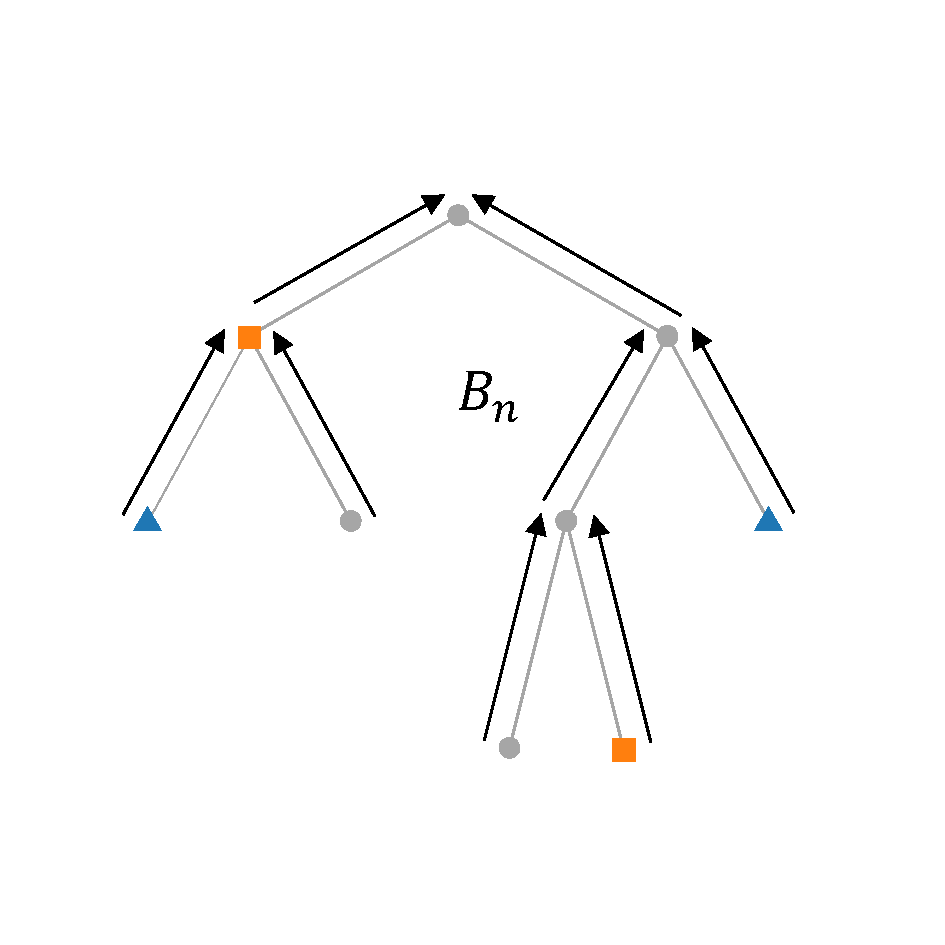
\includegraphics[trim={2.0cm 2.9cm 2.5cm 3.1cm}, clip,width=0.44\linewidth]{img/gbop/tree_2}
	\hfill
	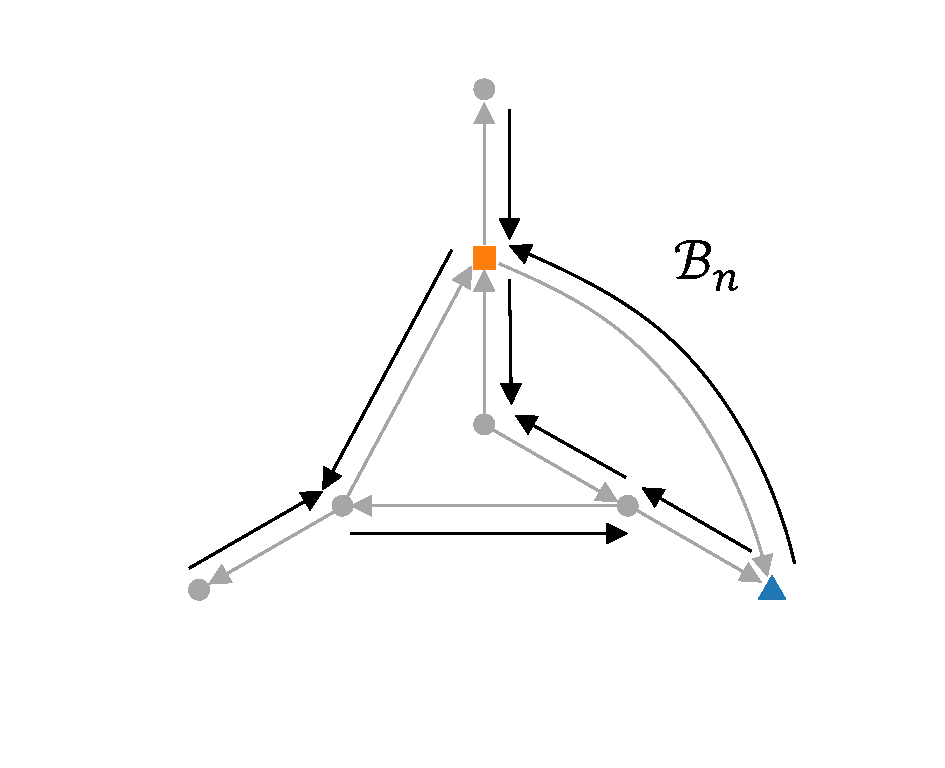
\includegraphics[trim={2.7cm 2.7cm 2.7cm 1.1cm}, clip,width=0.44\linewidth]{img/gbop/graph_2}
	\caption{Illustration of the Bellman backup operators $B$ (left) and $\cB$ (right). Notice that $B_n$ only propagates information upward in the tree.}
	\label{fig:bellman}
\end{figure}

\citet{Hren2008optimistic} used this Bellman operator $B_n$ in their \OPD algorithm to define a pair of bounds $(L_n,\, U_n)$ at each iteration $n$. They use trivial bounds at the leaves, and backup these estimates up to the root by iteratively applying $B_n$. We can show that, under a \textit{monotonicity} condition (satisfied by the trivial bounds $0$ and $V_{max}$), applying $B_n$ can only tighten a bound and converges in a finite time.

\begin{definition}[Monotonicity]
	\begin{leftbar}[defnbar]
	A pair of bounds ($L$, $U$) or $(\cL, \cU)$ is \emph{monotonic} if they are respectively non-decreasing and non-increasing along transitions:
	\begin{align*}
	\forall a\in{\Tau}_n, \quad & L(a) \leq B_n(L)(a), & U(a) & \geq B_n(U)(a)\\
	\forall (s)\in\inte{\cG}_n, \quad &\; \cL(s) \leq \cB_n(\cL)(s),&   \cU(s) & \geq \cB_n(\cU)(s)
	\end{align*}
	\end{leftbar}
\end{definition}

\begin{lemma}[Properties of $B_n$]
	\begin{leftbar}[lemmabar]
	\label{lem:properties-b-tree}
	\begin{enumerate}[label=(\roman*)]
		\item $B_n$ preserves monotonicity and tightens monotonic bounds: $$
		\text{if } L\leq V\leq U \text{, then } L \leq B_n(L) \leq V \leq B_n(U) \leq U;
		$$
		\item The sequence $B_n^k = \underbrace{B_n \circ \dots\circ B_n}_{\text{$k$ times}} $ converges in a finite time $k=d_n$, where $d_n$ is the depth of $T_n$. 
	\end{enumerate}
	\end{leftbar}
\end{lemma}
This enables \citet{Hren2008optimistic} to define\footnote{We use an iteration of operators while a recursive definition was used originally.} non-trivial valid bounds on $V$:
\begin{align}
\label{eq:opd-bounds}
L_n \eqdef B_n^{d_n}(0), \qquad U_n \eqdef B_n^{d_n}(V_{\max}),
\end{align}
where $0$ is the null function.
The corresponding \texttt{OPD} algorithm is described in \Cref{alg:opd}.

\begin{algorithm}[!ht]
	\caption{The \emph{Optimistic Planning of Deterministic Systems} (\OPD) algorithm from \citep{Hren2008optimistic}.}
	\label{alg:opd}
	\DontPrintSemicolon
	\For{each iteration $n$}{
		Compute the bounds $L_n = B_n^{d_n}(0)$ and $U_n = B_n^{d_n}(V_{\max})$.\; 
		
		$b_n\gets \emptyset$\;
		
		\While{the node $b_n\in\inte{\Tau}_n$ is internal}{
			$b_n\gets \displaystyle\argmax_{a'\in b_n A} r(a') + \gamma U_n(a')$ \Comment*[r]{Optimistic sampling rule}
		}
		\For(\Comment*[f]{Node expansion}){action $a\in \cA$}{
			Simulate $r \gets r(s(b_n),a)$ and $s' \gets P(s(b_n),a)$.\;
			
			Add a new leaf $b_n a$ to $\Tau_{n+1}$, with associated reward $r$.\;
		}
	}
	\Return $\displaystyle\argmax_{a\in \cA} r(s, a) + \gamma L_n(a)$. \Comment*[r]{Conservative recommendation rule}\;
\end{algorithm}


 Likewise, we show that the graph version $\cB_n$ verifies similar properties.
\begin{lemma}[Properties of $\cB_n$]
	\begin{leftbar}[lemmabar]
	\label{lem:properties-b-graph}
	\begin{enumerate}[label=(\roman*)]
		\item $\cB_n$ preserves monotonicity and tightens monotonic bounds: $$
		\text{if } \cL\leq V\leq \cU \text{, then } \cL \leq \cB_n(\cL) \leq V \leq \cB_n(\cU) \leq \cU;
		$$
		\item $\cB$ is a $\discount$-contraction, and we denote $\cB_n^{\infty} \eqdef \lim_{k\rightarrow \infty} \cB_n^k$.
	\end{enumerate}
	\end{leftbar}
\end{lemma}
This motivates us to propose \Cref{alg:gbop-d}, following the approach of \Cref{alg:opd} adapted to a graph structure.

\begin{algorithm}[!ht]
	\caption{Our proposed \emph{Graph-Based Optimistic Planning for Deterministic systems} (\GBOPD) algorithm.}
	\label{alg:gbop-d}
	\DontPrintSemicolon
	\For{each iteration $n$}{
		\nl Compute the bounds $\cL_n = \cB_n^{\infty}(0)$ and $\cU_n = \cB_n^\infty(V_{\max})$.\; 
		
		$s_n \gets s_1$\;
		
		\While{the node $s_n\in\inte{\cG}_n$ is internal}{
			\nl $s_n\gets \displaystyle\argmax_{s'} r(s_n, a) + \gamma \cU_n(s')$ \Comment*[r]{Optimistic sampling rule}
		}
		\For(\Comment*[f]{Node expansion}){action $a\in \cA$}{
			Simulate $r \gets r(s_n, a)$ and $s' \gets P(s_n,a)$.\;
			
			Get or create the node $s'$ in $\cG_{n+1}$, and add the transition $(s_n,a) \rightarrow s', r$.\;
		}
	}
	\Return $\displaystyle\argmax_{a\in \cA} R(s,a) + \discount \cL_n(s(a))$. \Comment*[r]{Conservative recommendation rule}
\end{algorithm}

\begin{remark}[Termination and complexity]
	\begin{leftbar}[remarkbar]
	There are two procedures in \GBOPD that may not terminate in finite time when $\cG_n$ contains a loop:
	% \begin{enumerate*}[label=(\roman*)
		the computation of $\cB_n^\infty$ (line 1) and
		the sampling rule loop (line 2).
	% \end{enumerate*}
	We handle these steps carefully in \Cref{sec:gbop-implementation}, where we discuss an approximate implementation in which these two procedures are stopped whenever they reach a desired accuracy $\varepsilon$, along with an analysis of the corresponding time complexity and impact on the performance.
	\end{leftbar}
\end{remark}

Though both algorithms share a similar design, we claim that using graphs provides substantial theoretical and practical performance improvements, and back up this statement in \Cref{sec:gbop-analysis,sec:gbop-experiments}.

\subsection{Analysis}
\label{sec:gbop-analysis}

Comparing \OPD and \GBOPD directly is difficult since they do not involve the same structure, which implies implicit differences in their behaviours. Studying them under a common framework makes these differences explicit. To leverage the analysis of \OPD by \citet{Hren2008optimistic}, we will frame \GBOPD as a tree-based planning algorithm: the graph operator $\cB$ will be represented as tree backup $B$ applied on an \emph{unrolled} tree $T(\cG_n)$, defined below.

\subsubsection{Background on the sample complexity of \OPD}

First, we recall the analysis of \citet{Hren2008optimistic} and introduce some notations.

\begin{lemma}[Sequence values]
	\begin{leftbar}[defnbar]
	The value of a finite \textbf{sequence} of actions $a\in \cA^h$, defined in \Cref{def:sequence-values}, verifies
	\begin{equation*}
	\label{eq:state_value}
	V(a) = G(s_1,a) + \discount^{h} V(s(a)),
	\end{equation*}
	where $G(s, a) = \sum_{t=0}^{h-1} \discount^t r_t$ is the return obtained by executing the sequence of actions $a$ starting from the state $s$.
	\end{leftbar}
\end{lemma}

This enables to define a measure of the difficulty of a planning problem.

\begin{definition}[Difficulty measure]
	\begin{leftbar}[defnbar]
	We define the near-optimal branching factor $\hlrb{\kappa}$ of an MDP as
	\begin{equation}
	\hlrb{\kappa = \limsup_{h\rightarrow\infty} |\hlrb{\Tau_h^\infty}|^{1/h}} \in [1, K]
	\end{equation}
	where $\Tau^\infty_h = \displaystyle \left\{a\in \cA^h: V^\star-V(a) \leq \frac{\discount^h}{1-\discount}\right\}$ is the set of near-optimal nodes at depth $h$.
	\end{leftbar}
\end{definition}

This problem-dependent measure $\hlrb{\kappa}$ is the branching factor of the subtree $T^\infty=\bigcup_h T_h^\infty$ of near-optimal nodes that can be sampled by \OPD, and acts as an effective branching factor as opposed to the true branching factor $K$. When $\hlrb{\kappa}$ is small, fewer nodes must be explored at a given depth allowing the algorithm to plan deeper for a given budget $n$. Thus, it directly impacts the simple regret that can be achieved by \OPD when run on a given MDP.


\begin{theorem}[Regret bound of \citealt{Hren2008optimistic}]
	\begin{leftbar}[theorembar]
	\label{thm:regret-opd}
	The \Cref{alg:opd} enjoys the following regret bound:
	\begin{align*}
	\regret = \tilde{\cO}\left( n^{-\log \frac{1}{\discount}/\hlrb{\log\kappa}}\right),
	\end{align*}
where $f_n = \tilde{\cO}(n^{-\alpha})$ means that for any $\alpha'<\alpha$, $f_n = \cO(n^{-\alpha'})$, for all $\alpha\in \Real_+ \cup \{+\infty\}$.
	\end{leftbar}
\end{theorem}

The near-optimal branching factor $\hlrb{\kappa}$ is related \citep{Bubeck2010} to the near-optimality dimension studied in the online optimisation literature \citep[see e.g.][]{Bubeck2009,Munos2011}.
It is typically small in problems where there is one single optimal trajectory, of which any deviation can be quickly dismissed as suboptimal. Conversely, $\kappa$ is large when many sub-optimal trajectories cannot be distinguished easily based on their values, which requires the exploration of a large part of the tree $T$ of branching factor $K$. 


\subsubsection{Motivation for an improved regret bound}

We start by reformulating the sampling rule used for the \texttt{OPD} algorithm. To that end, notice that when some bounds $(L,\,U)$ on the state values $V(s(a))$ are available, they also induce bounds $(\overline{L},\, \overline{U})$ on values $V(a)$ of sequences of actions $a$ of length $h$ defined as
\begin{equation*}
%\label{eq:sequence_value}
\underbrace{R(s_1,a) + \discount^{h} L(a)}_{\overline{L}(a)} \leq V(a) \leq \underbrace{R(s_1,a) + \discount^{h} U(a)}_{\overline{U}(a)}.
\end{equation*}

One can easily see that, since the $(L_n,\,U_n)$ used in the optimistic sampling rule described in \Cref{alg:opd} are invariant by $B_n$ by definition, this rule can be equivalently expressed as
\begin{equation}
\label{eq:sampling_rule}
b_n \in \argmax_{a\in\ext{\Tau}_n} \overline{U}_n(a).
\end{equation}
Likewise, the conservative recommendation rule returns the first action of
\begin{equation}
\label{eq:recommendation_rule}
a_n \in \argmax_{a\in\ext{\Tau}_n} \overline{L}_n(a)
\end{equation}


As shown in \Cref{fig:bellman}, in a tree the Bellman operator $B_n$ only propagates the information upward, and the leaves cannot be updated. Thus, $U_n = B_n^{d_n}(V_{\max})$ and $V_{\max}$ coincide on $\ext{\Tau}_n$ which means that the sampling rule of \texttt{OPD} can be summarized as using \eqref{eq:sampling_rule} with the trivial upper-bound $U_n = V_{\max}$.
Likewise, the recommendation rule simply uses \eqref{eq:recommendation_rule} with the trivial lower-bound $L_n = 0$. Thus, \texttt{OPD} amounts to simply using the trivial bound $(0,\, V_{\max})$ on leaf nodes, and does not make use of all the available information in $\Tau_n$ to improve these bounds.

Let us now assume for the moment that we had access to tighter bounds $(L,\,U)$ provided by an oracle: $$0\leq L\leq V\leq U\leq V_{\max}.$$

\begin{definition}[A finer difficulty measure]
	\begin{leftbar}[defnbar]
	We define the near-optimal branching factor \emph{according to the bounds $(L,\,U)$} as 
	\begin{equation}
	\hlbb{\kappa(L,U) \eqdef \limsup_{h\rightarrow\infty} \left|\Tau_h^\infty(L,U)\right|^{1/h}}\in(1, K], 
	\end{equation}
	where
	$ \displaystyle
	{\Tau_h^\infty(L,U)}=\left\{a\in \cA^h: V^\star - V(a)\leq \discount^{h}(U(a)-L(a))\right\}.
	$
	\end{leftbar}
\end{definition}

\begin{lemma}
	\begin{leftbar}[lemmabar]
	\label{lem:shrink}
	This branching factor shrinks as the bounds $(L,\,U)$ get tighter:
	\[L_2\leq L_1\leq V\leq U_1\leq U_2\implies \kappa(L_1,U_1) \leq \kappa(L_2,U_2).\]
	In particular, $\hlbb{\kappa(L,U)} \leq \hlrb{\kappa}$.
	\end{leftbar}
\end{lemma}

\begin{theorem}
	\begin{leftbar}[theorembar]
	\label{thm:regret-bound-U}
	Let $L \leq V\leq U$ monotonic bounds, then planning with $L$ and $U$ in \eqref{eq:sampling_rule} and \eqref{eq:recommendation_rule} yields the following simple regret bound:
	\begin{equation*}
	\regret = \tilde{\cO}\left(n^{-\log \frac{1}{\discount}/\hlbb{\log \kappa(L,U)}}\right).
	\end{equation*}
	\end{leftbar}
\end{theorem}


This theorem states that we can potentially improve the performance of the planning algorithm if we manage to find bounds $(L,\, U)$ that are tighter than the trivial ones at the leaves $\ext{\Tau_n}$, which may be possible if we have already seen the states corresponding to this leaves, but it does not explain how to obtain such bounds. In the next subsection, we describe a method to build a sequence of increasingly tight bounds $(L_n,\, U_n)$, at each planning iteration $n$. The corresponding regret bound, our main result, is stated in \Cref{thm:regret-gbop}.


\subsubsection{Unrolling the tree to tighten the bounds}
\label{sec:unrolling}

In order to reproduce the behaviour of \Cref{alg:gbop-d} on a tree structure, we rely on the following observation:  expanding a node $s$ in $\cG_n$ simultaneously expands all the paths leading to this node.
To account for this observation in the analysis, we will consider an \emph{unrolling} operator $T$ that builds a potentially infinite tree $T(\cG_n)$ containing every sequence of action that can be traversed in a graph $\cG_n$.

\begin{equation}
T(\cG_n) = \{a\in \cA^h: s_{t+1} \in \cG_n \text{ with } s_{t+1} = P(s_{t}, a_t)\text{ for } 0 \leq t < h\}
\end{equation}

\begin{figure}[htp]
	\centering
	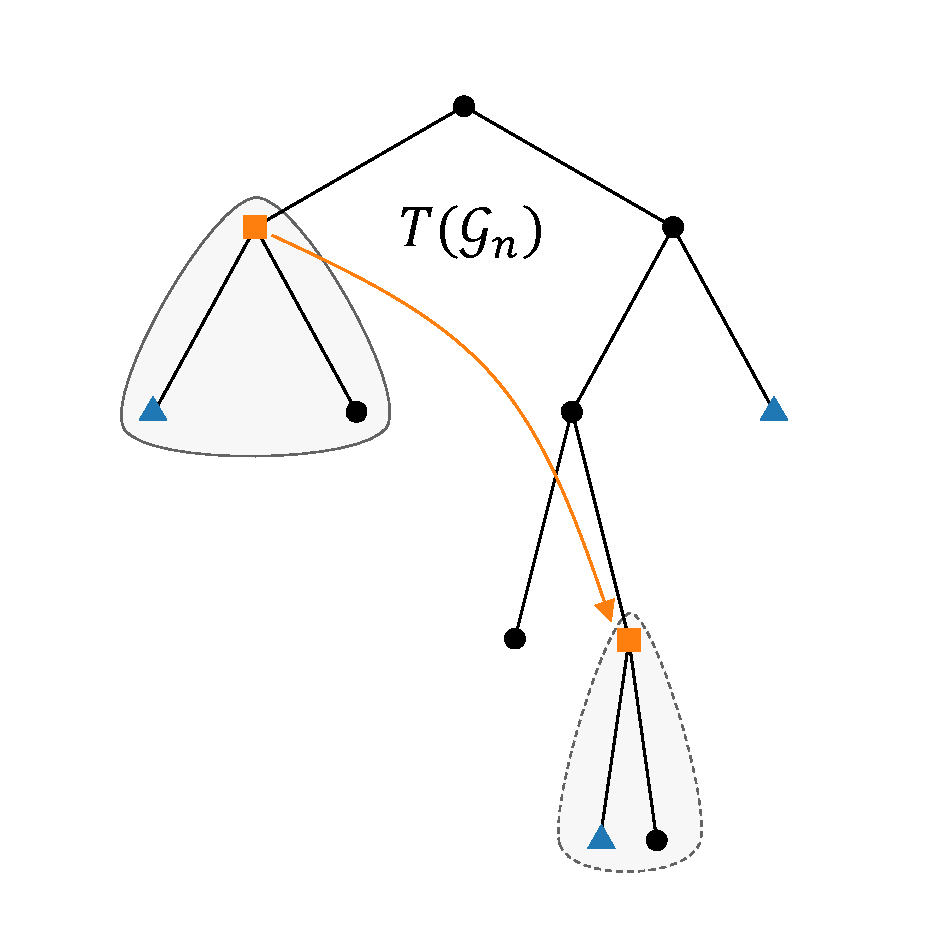
\includegraphics[trim={2.cm 1cm 2.5cm 1cm}, clip, width=0.44\textwidth]{img/gbop/tree_5.pdf}
	\caption{The tree $T(\cG_n)$ obtained by unrolling $\cG_n$. Contrary to $T_n$ shown in \Cref{fig:structures}, the red leaf $a$ is expanded at the same time as the internal red node, which enables to tighten its value bounds $(L_n(a), U_n(a))$ by applying $B_n$.}
	\label{fig:unroll}
\end{figure}
We analyse \GBOPD though the prism of $T(\cG_n)$, which is only used as a theoretical tool. 

We can define the counterpart of the bounds $(\cL_n, \cU_n)$ in the same way as \eqref{eq:opd-bounds} applied to $T(\cG_n)$ rather than $T_n$, except that the depth $d_n$ of $T(\cG_n)$ can now be infinite:
\begin{align}
\label{eq:gbop-t-bounds}
L_n = B_n^{\infty}(0), \qquad U_n = B_n^{\infty}(V_{\max}).
\end{align}
This definition is equivalent to that of \GBOPD in the sense that
\begin{lemma}[Bound equivalence]
	\label{lem:equivalence}
	For any sequence of action $a\in T(\cG_n)$, we have $L_n(a) = \cL_n(s(a))$ and $U_n(a) = \cU_n(s(a))$.	
\end{lemma}

In $T(\cG_n)$, the unrolling mechanics behave as if any leaf $a$ sharing the same state $s(a)$ as an internal node $a'$ was automatically expanded, and thus had its bound $L_n(a), U_n(a)$ tightened by the Bellman backup $B_n$ to a sub-interval of the trivial bounds $(0, V_{\max})$ that are used in \OPD.

The sampling and recommendation rules of \GBOPD also amount to running those of \OPD on the tree $T(\cG_n)$, except that the sampled sequence $b_n$ and recommended sequence $a_n$ can now have infinite depth since $T(\cG_n)$ itself can be infinite (we say that $a_n$ and $b_n$ are represented by nodes of infinite depth). In the sequel, we analyse how these rules behave on $T(\cG_n)$.

\begin{lemma}[Expansion]
	\begin{leftbar}[lemmabar]
	\label{lem:expansion-bound}
	Any node $a$ of depth $h$ traversed by the optimistic sampling rule of \GBOPD at iteration $n$ belongs to $T_h^\infty(L_n, U_n)$: 
	\begin{equation}
	\label{eq:expansion-regret}
	V^\star-V(a) \leq \discount^h(U_n(a)-L_n(a)).
	\end{equation}
	
	In particular, if the sampling rule samples an infinite sequence $a\in \cA^\infty$, it is an optimal sequence, and we write that \eqref{alg:gbop-d} also holds for $a$ with $h=\infty$.
	\end{leftbar}
\end{lemma}


\begin{lemma}[Recommendation]
	\begin{leftbar}[lemmabar]
	\label{lem:recommendation-bound}
	The action $a_n$ recommended by \GBOPD has a simple regret $\regret \leq \frac{\discount^{d_n}}{1-\discount}$, where $d_n\in\Real\cup\{\infty\}$ is the maximal depth of expanded nodes in $T(\cG_n)$.
	\end{leftbar}
\end{lemma}
Note that even though $T(\cG_n)$ can be infinite, there is only one node $b_t$ that is selected for expansion at each iteration $t\leq n$.

\subsubsection{Regret guarantee}

In \Cref{thm:regret-bound-U}, we assumed that some bounds $(L,\,U)$ were revealed by an oracle and available from the onset for planning. In \eqref{eq:gbop-t-bounds}, we instead built a \emph{sequence} of bounds $(L_n,U_n)_{n\geq 0}$ \eqref{eq:gbop-t-bounds} that is non-increasing in the sense of inclusion, i.e. $0\leq \dots\leq L_{n-1}\leq L_n\leq V\leq U_n\leq U_{n-1}\leq \dots\leq V_{\max}$.

We can consider the sequence $\kappa_n = \kappa(L_n, U_n)$. It is non-increasing and lower-bounded by $1$, thus converges. Let $\hlgb{\kappa_\infty = \lim_{n\rightarrow\infty} \kappa(L_n, U_n)} \in[1,K]$.

\begin{theorem}
	\begin{leftbar}[theorembar]
	\label{thm:regret-gbop}
	\GBOPD enjoys the following regret bound, with $\hlgb{\kappa_\infty} \leq \hlrb{\kappa}$: 
	\begin{align*}
	\regret = \tilde{\cO}\left(n^{-\log \frac{1}{\discount}/\hlgb{\log \kappa_\infty}}\right).
	\end{align*}
	\end{leftbar}
\end{theorem}

Intuitively, $\kappa_\infty$ should be much lower than $\kappa$ in problems where trajectories overlap a lot. For instance, it will be the case for problems where two actions cancel each-other out (e.g. moving left or right), or are commutative (e.g. placing pawns on a board game). However, this is merely an intuition. We now show that there exist problem instances in which $\hlgb{\kappa_\infty} < \hlrb{\kappa}$, which is a legitimate concern since their non-existence would make \Cref{thm:regret-gbop} trivial.

\subsubsection{Illustrative example}

In Proposition \ref{prop:illustrative-example}, we consider a toy MDP $\cM$ shown in \Cref{fig:mdp}. The transitions are described visually while the rewards are defined as follows: let $0\leq r^\star\leq \gamma$, and $ r^- = r^\star - \frac{\gamma}{1-\gamma} S$, $r^+ = r^\star + S$ with $S = r^\star\left(\frac{1}{\gamma} - 1\right).$ Note that this choice ensures that $r^\star, r^-, r^+$ and $S$ are all in $[0, 1]$.

\begin{figure}[htp]
	\centering
	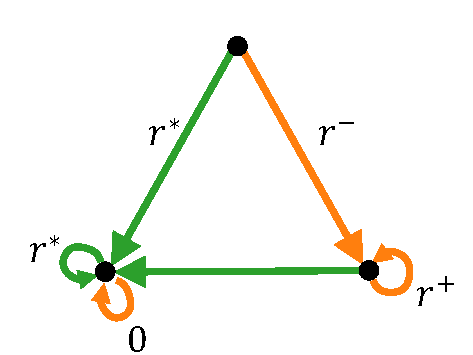
\includegraphics[trim={0.5cm 0.0cm 0.3cm 0.6cm}, clip, width=0.35\textwidth]{img/gbop/mdp.pdf}
	\caption{A toy MDP with three states and $K \geq 2$ actions. We start in the top state. The first action $a_1$ is represented by \hlg{green} arrows, and all other actions $a_2, \dots, a_K$ are represented by \hlo{orange} arrows. The rewards are shown next to the transitions.}
	\label{fig:mdp}
\end{figure}

\begin{proposition}[Branching factors]
	\begin{leftbar}[propositionbar]
	\label{prop:illustrative-example}
	The MDP $\cM$ verifies $\hlrb{\kappa = K-1}$ and $\hlgb{\kappa_\infty = 1}$.
	%
	% \begin{enumerate}[label=(\roman*)]
	%     \item $\hlrb{\kappa = K-1}$;
	%     \item $\hlgb{\kappa_\infty = 1}$.
	% \end{enumerate}
	\end{leftbar}
\end{proposition}
This result confirms that \Cref{thm:regret-gbop} is non-trivial since we exhibit a problem for which $\hlgb{\kappa_\infty} < \hlrb{\kappa}$ (when $K\geq 3$), and legitimates our attempt to improve planning performances by merging the tree into a graph.


\subsection{Extension to Stochastic Systems}
\label{sec:gbop-stochastic}

The approach developed in \Cref{sec:gbopd,sec:analysis} consists in using state similarity to tighten a pair of lower and upper bounds $(L,\,U)$ for the value function $V$. Thus, any planning algorithm that is based on such bounds can benefit from this insight, and any theoretical result based on the validity and rate of convergence of these bounds will be preserved.  

\paragraph{Confidence intervals for rewards.}

% TODO: say that rewards can be stochastic
When the reward kernel $P\left(r \condbar s,a\right)$ is stochastic, deviation inequalities can be used to design a confidence interval $[\ell_t(s,a), u_t(s,a)]$ over its expected value $\expectedvalue\left[r | s,a\right]$. For instance, the Chernoff-Hoeffding deviation inequality was used to design confidence intervals in \citep{Kocsis06UCT,Bubeck2010,Kaufmann2017}.
In recent works \citep{Leurent2019practical, Jonsson2020planning}, the tighter Kullback-Leibler confidence interval is preferred:
\begin{align*}
u_t(s,a) &\eqdef \max \left\{v : \kl\!\big(\hat{r}_t(s,a),v\big) \leq \frac {\beta^r(n_t(s,a), n)} {n_t(s,a)} \right\},\\
\ell_t(s,a) &\eqdef\min \left\{v : \kl\!\big(\hat{r}_t(s,a),v\big) \leq \frac {\beta^r(n_t(s,a), n)} {n_t(s,a)} \right\},
\end{align*}
where $\hat{r}_t(s,a)$ is the sample mean, $\beta^r$ is an exploration function and $\kl(u,v)$ is the binary Kullback-Leibler divergence between Bernoulli distributions: $\kl(u,v) = u \log \tfrac {u} {v} + (1-u) \log \tfrac {1-u} {1-v}$.

\paragraph{Confidence region for transitions.}

Likewise, when the transition kernel $P\left(s' \condbar s,a\right)$ is stochastic, a confidence set on the probability vector $p(\cdot|s,a)$ can be defined as
$$\cC_t(s,a) \eqdef \left\{p\in \Sigma_S :  \KL\!\big(\hp_t(\cdot|s,a),p\big) \leq \frac {\beta^p(n_t(s,a), n)} {n_t(s,a)}\right\},$$
where $\hp_t(\cdot|s,a) \eqdef n_t(s,a,\cdot) / n_t(s,a)$ is the empirical distribution, $\Sigma_S$ is the probability simplex over $S$, $\beta^p$ is an exploration function and $\KL(p,q)= \sum_{s \in S}  p(s) \log \tfrac{ p(s)} {{q}(s)}$ is the Kullback-Leibler divergence between categorical distributions.

\paragraph{Bellman operator with stochasticity.}

In this work, we do not discuss the tuning of $\beta^r$, $\beta^p$, but simply assume that they are chosen such that the rewards and transitions belong to their confidence regions with sufficiently high probability to obtain performance guarantees for the  planning algorithm. For more details on such a choice, refer to \citep[e.g.][]{Leurent2019practical, Jonsson2020planning}. We modify the \Cref{def:bellman} of the Bellman operator on graphs $\cB_t$ as
\begin{align*}
\cB_t^+(\cU)(s) &= \max_{a\in \cA} \left[u_t(s,a) + \gamma \max_{q \in \cC_t(s,a)} \sum_{s'} q(s'|s,a) \cU(s')\right], \\
\cB_t^-(\cL)(s) &= \max_{a\in \cA} \left[\ell_t(s,a) + \gamma \min_{q \in \cC_t(s,a)} \sum_{s'} q(s'|s,a)\cL(s')\right],
\end{align*}
for all $s\in\inte{\cG_n}$, where the maximum and minimum over these Kullback-Leibler confidence regions $\cC_t(s,a)$ can be computed as explained in \citep[Appendix A of][]{Filippi2010optimism}. Under the event that every confidence regions $[\ell_t(s,a), u_t(s,a)]$ and $\cC_t(s,a)$ are valid at time $t$, the \Cref{lem:properties-b-graph} still holds for $\cB_t^-, \cB_t^+$.

\paragraph{Structure of the planning algorithm}

In the deterministic setting, once a transition has been observed, it is known with certainty and doesn't need to be sampled ever again, which is why only external nodes $\ext{\cG_n}$ are sampled in \GBOPD. Conversely, in the stochastic setting the expected reward and transition probabilities must be estimated from samples, which implies that internal nodes $\inte{\cG_n}$ must be sampled as well. Then, it is common to adopt and episodic setting where we sample trajectories of a fixed horizon $H$, tuned depending on the budget $n$. This is the case in  \citep[e.g.][]{Kearns02SS,Kocsis06UCT,Bubeck2010,Feldman14BRUE,Leurent2019practical,Jonsson2020planning}. We also follow this scheme in our proposed \Cref{alg:gbop}.

\begin{algorithm}[ht]
	\caption{\emph{Graph-Based Optimistic Planning} (\GBOP) algorithm.}
	\label{alg:gbop}
	\DontPrintSemicolon
	\For{trajectory $m$ in $[1, M]$}{
		\For{time $t$ in $[1, H]$}{
			$n \gets (m - 1)H + h$.\;
			Compute the bounds $\cL_n = (\cB_n^-)^{\infty}(0)$ and $\cU_n = (\cB_n^+)^\infty(V_{\max})$.\; 
			$b_t\gets \displaystyle\argmax_{a\in \cA} r(s_t, a) + \discount \cU_n(s')$ \Comment*[r]{Optimistic sampling rule}
			Simulate $r_t, s_{t+1} \sim P\left(r, s_{t+1} \condbar s_t, b_t\right)$.\;
			Get or create the node $s_{t+1}$ in $\cG_{n+1}$, and add an occurence of the transition $(s_t,b_t, r_t, s_{t+1})$.
		}
	}
	\Return $\displaystyle\argmax_{a\in \cA} r(s,a) + \discount \cL_n(s(a))$. \Comment*[r]{Conservative recommendation rule}
\end{algorithm}

\subsection{Numerical Experiments}
\label{sec:gbop-experiments}

To evaluate the practical benefits of our approach, we compare graph-based and tree-based planning algorithms in various problems.

\begin{figure}[ht]
	\centering
	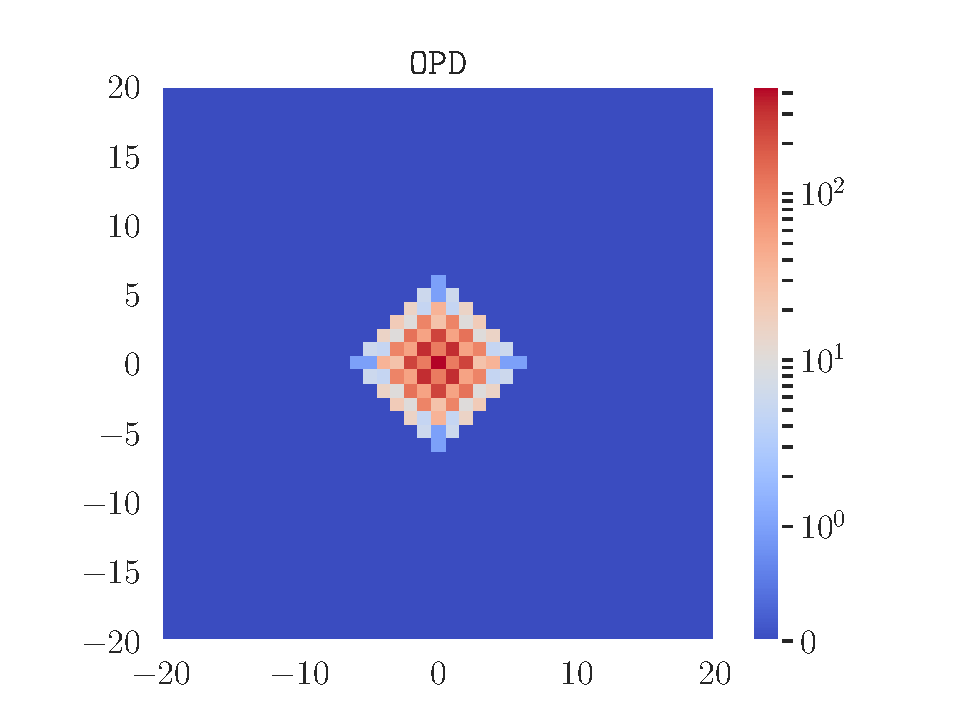
\includegraphics[trim={1.8cm 0.4cm 1.8cm 0.7cm}, clip, width=0.45\linewidth]{img/gbop/occupations_OPD.pdf}
	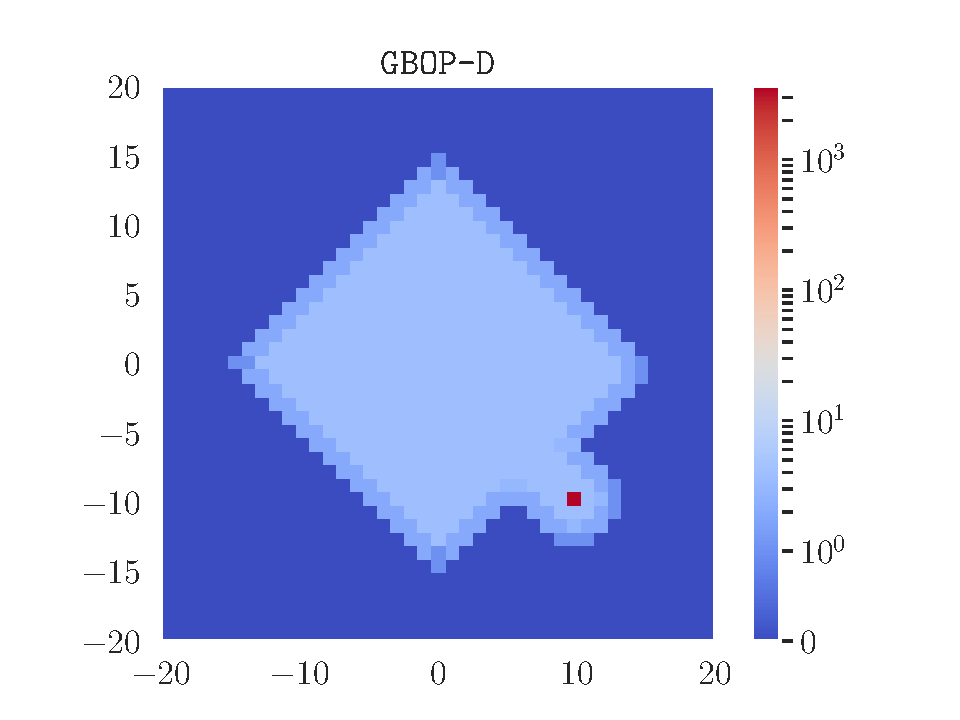
\includegraphics[trim={1.8cm 0.4cm 1.8cm 0.7cm}, clip, width=0.45\linewidth]{img/gbop/occupations_GBOP-D.pdf}
	\caption{State occupancies of tree-based \vs graph-based algorithms in a deterministic gridworld.}
	\label{fig:deterministic-gridworld}
\end{figure}

\paragraph{Parameters.} In every experiment, we used $\gamma=0.95$. In \GBOPD and \GBOP, the fixed accuracy $\varepsilon=\num{1e-2}$ was used for computing $\cB_n^\infty$, and the sampling rule was stopped after reaching the depth $d^+_n = n$ (see \Cref{sec:gbop-implementation}).
Regarding the tuning of confidence intervals in \GBOP, since the rewards are deterministic and the transitions are stochastic in both domains we used $\beta^r(n_t(s,a), n) = 0$ and $\beta^p(n_t(s,a), n) = \log n$, following the observations of \Cref{sec:kl-olop}. The maximal size $B$ of the support of the transitions $\Ps\left(s'|s,a\right)$ was also used ($B=4$ in the gridworld domain and $B=3$ in the sailing domain) to accelerate the computations of the confidence region $\cC_t$ for transitions, as explained in \citep{Jonsson2020planning}.

\begin{figure}[ht]
	\centering
	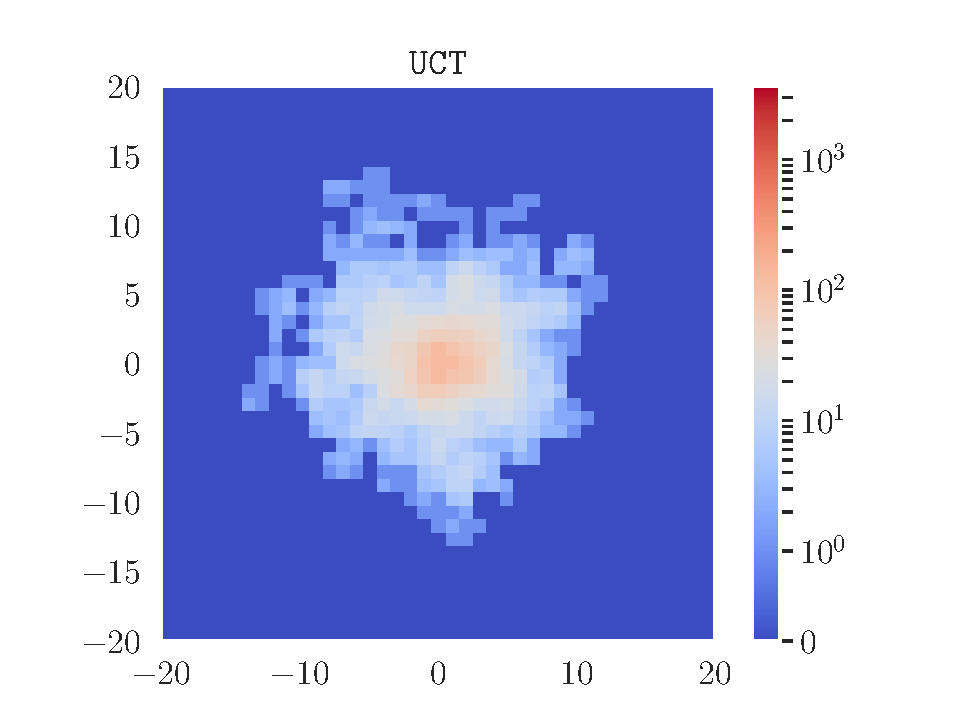
\includegraphics[trim={1.8cm 0.4cm 1.8cm 0.7cm}, clip, width=0.45\linewidth]{img/gbop/occupations_UCT.pdf}
	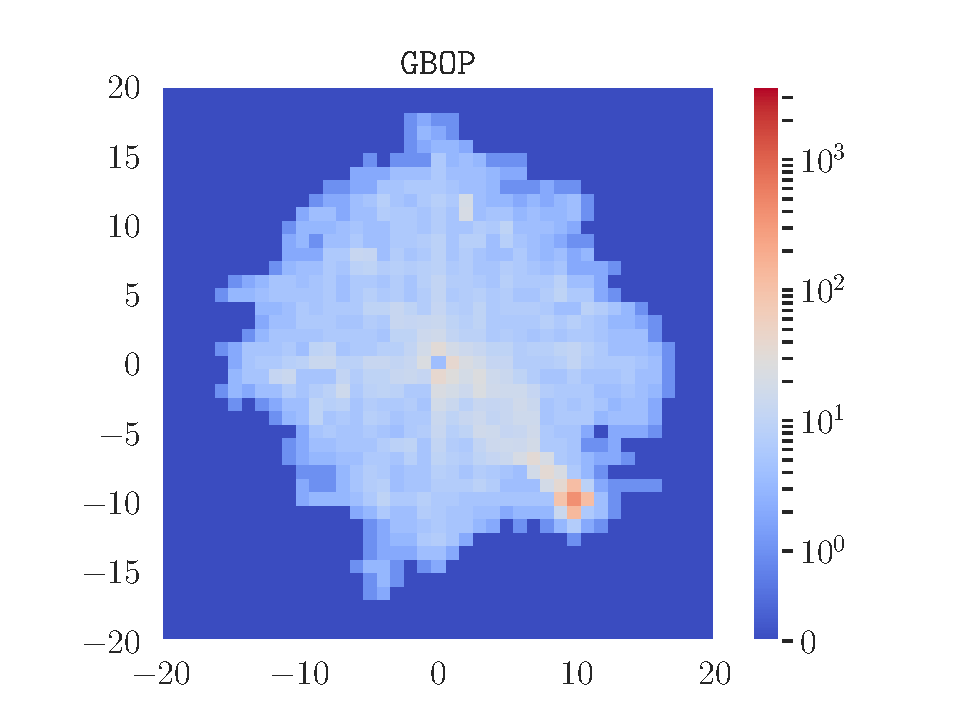
\includegraphics[trim={1.8cm 0.4cm 1.8cm 0.7cm}, clip, width=0.45\linewidth]{img/gbop/occupations_GBOP.pdf}\\
	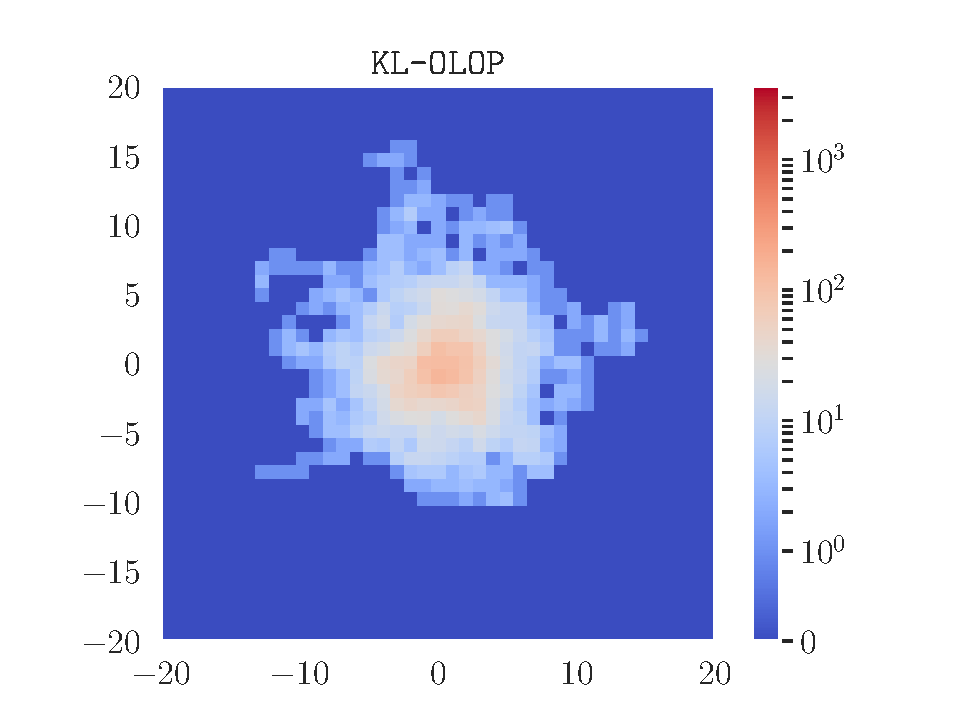
\includegraphics[trim={1.8cm 0.7cm 1.8cm 0.7cm}, clip, width=0.32\linewidth]{img/gbop/occupations_KL-OLOP.pdf}
	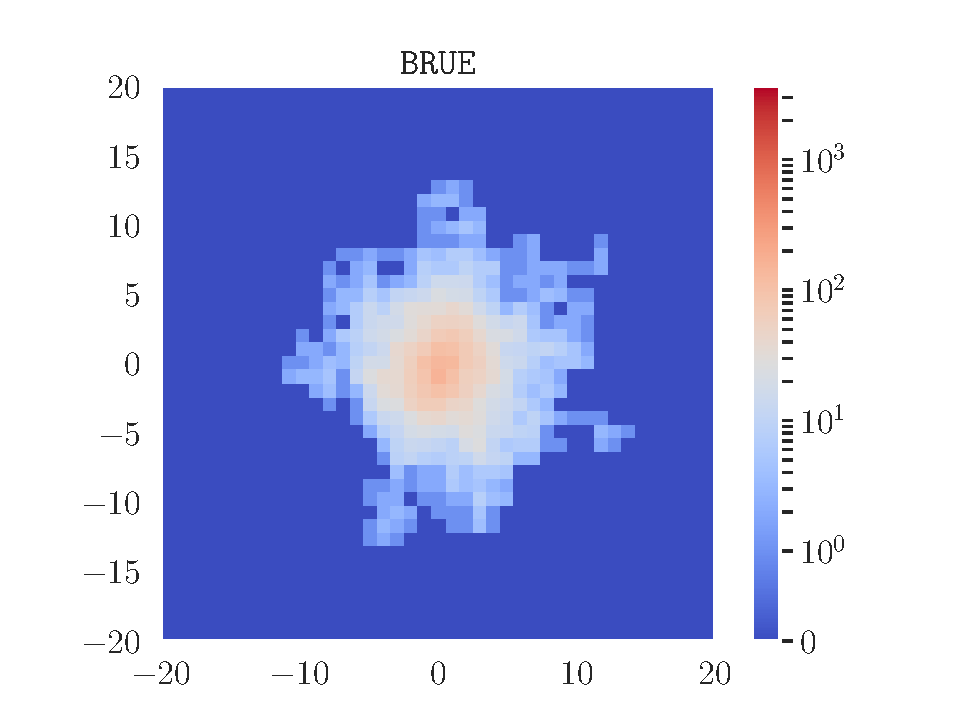
\includegraphics[trim={1.8cm 0.7cm 1.8cm 0.7cm}, clip, width=0.32\linewidth]{img/gbop/occupations_BRUE.pdf}
	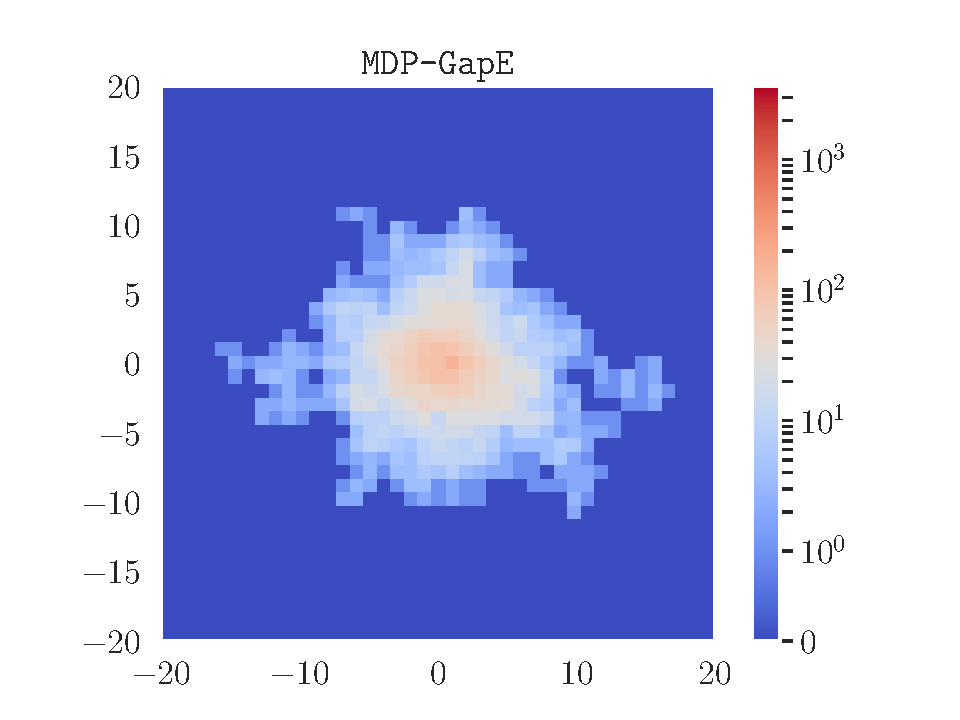
\includegraphics[trim={1.8cm 0.7cm 1.8cm 0.7cm}, clip, width=0.32\linewidth]{img/gbop/occupations_MDP-GapE.pdf}
	\caption{State occupancies of tree-based \vs graph-based algorithms in a stochastic gridworld.}
	\label{fig:stochastic-gridworld}
\end{figure}

\paragraph{Gridworld domain.}
We consider a grid in which the agent can move in $K=4$ directions. The reward function is $0$ everywhere, except in the vicinity of a goal located at $(10, 10)$, around which the reward decreases quadratically from $1$ to $0$ in a ball of radius $5$. %: $r(x, y) = \max(1 - \frac{1}{5^2}((x-10)^2 + (y-10)^2), 0)$. 
The \Cref{fig:deterministic-gridworld} shows number of times a state is sampled by \OPD and \GBOPD, both run with a budget $n = 5460$ and discount $\discount=0.95$. In the absence of rewards, \OPD samples sequences of actions uniformly (in a breadth-first search manner), which --because of the dynamics structure-- results in a non-uniform occupancy of the state space $S$, where the trajectories concentrate near the starting state. In contrast, \GBOPD explores uniformly in $S$, sampling each state up to four times (from its four  neighbours), until it finds the goal vicinity and finally samples the goal location indefinitely. We reproduce the experiment in the stochastic setting by adding noise on the transitions with probability $p=10\%$, and comparing \GBOP to \texttt{UCT} as we show in \Cref{fig:stochastic-gridworld}. To quantify these qualitative differences, we define in \Cref{fig:exploration-score} an exploration score: the mean distance $d(s_t, s_1)$ of sampled states to the initial state (exploration) minus the distance $d(s_t, s_g)$ to the goal state (exploitation).

\begin{figure}[ht]
	\centering
	\begin{subfigure}[b]{0.49\textwidth}
		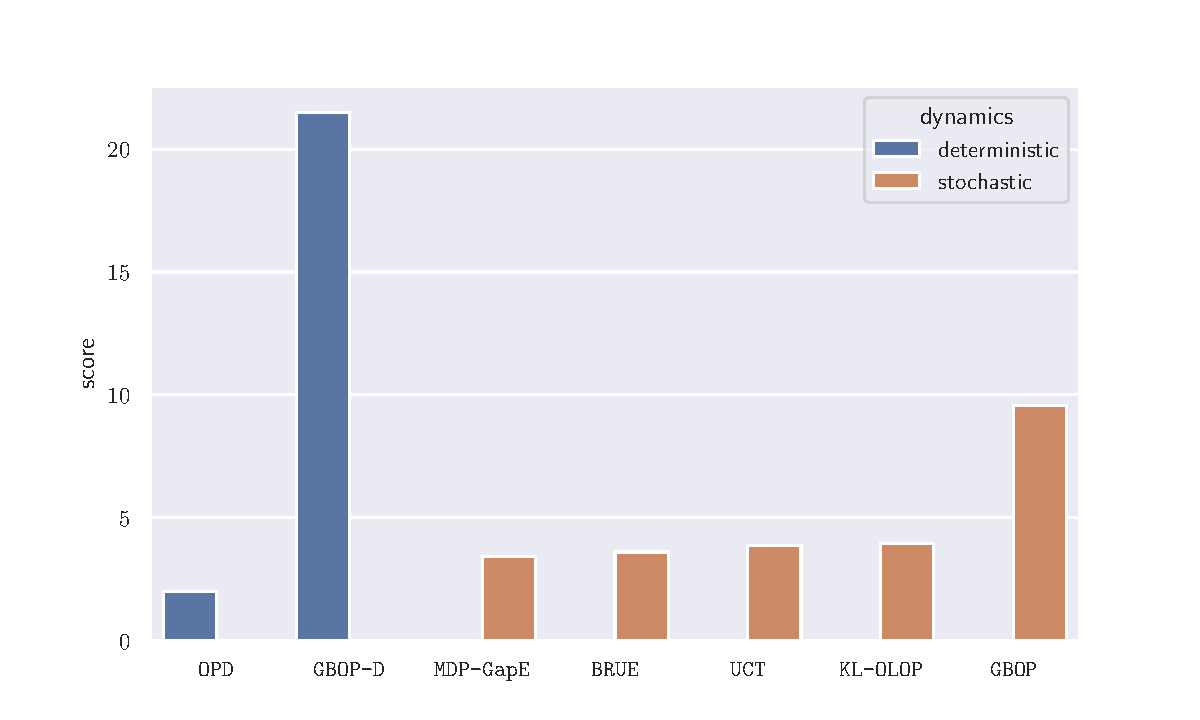
\includegraphics[trim = {1.6cm 0.cm 2cm 1.5cm}, clip, width=\linewidth]{img/gbop/score.pdf}
		\caption{Exploration score in the gridworld domain for several algorithms.}
		\label{fig:exploration-score}
	\end{subfigure}
	\hfill%
	\begin{subfigure}[b]{0.49\textwidth}
		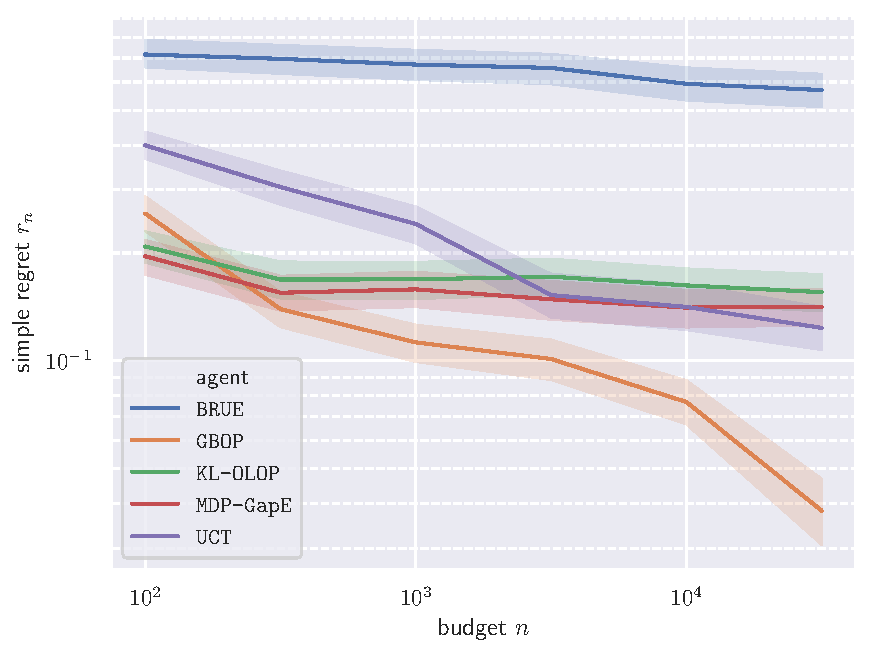
\includegraphics[trim = {0.2cm 0.2cm 0.7cm 0.5cm}, clip, width=\linewidth]{img/gbop/simple_regret.pdf}
		\caption{Mean simple regret $\regret$ in the sailing domain, with its $95\%$ confidence interval.}
		\label{fig:sailing}
	\end{subfigure}
	\caption{Benchmark of planning performances.}
\end{figure}


\paragraph{Sailing domain \citep{Vanderbei1996}.}
In a second experiment, a boat is sailing in $K=8$ directions to reach a goal, and suffers a cost (move duration) that depends on the direction of the wind which follows stochastic dynamics. \Cref{fig:sailing} shows the evolution of the simple regret $\regret$ of stochastic planning algorithms with respect to the number $n$ of oracle calls. We show the mean regret and its 95\% confidence interval computed over 500 simulations. The asymptotic log-log slope $\sigma$ provides an empirical measurement of the effective branching factor $\kappa_e = \exp(-\log(1/\discount)/\sigma)$ for each algorithm. We measure that for $n>10^{3.5}$, $\sigma \approx-0.04$ and $\kappa_e \approx 3.6$ for \gls{BRUE}, \KLOLOP, \gls{MDPGapE}, \gls{UCT}. In contrast, we measure $\sigma \approx-0.3$ and $\kappa_e \approx 1.2$ for \GBOP, which suggests that our result of \Cref{thm:regret-gbop} might generalize to the stochastic setting. 

\begin{figure}[p]
	\centering
	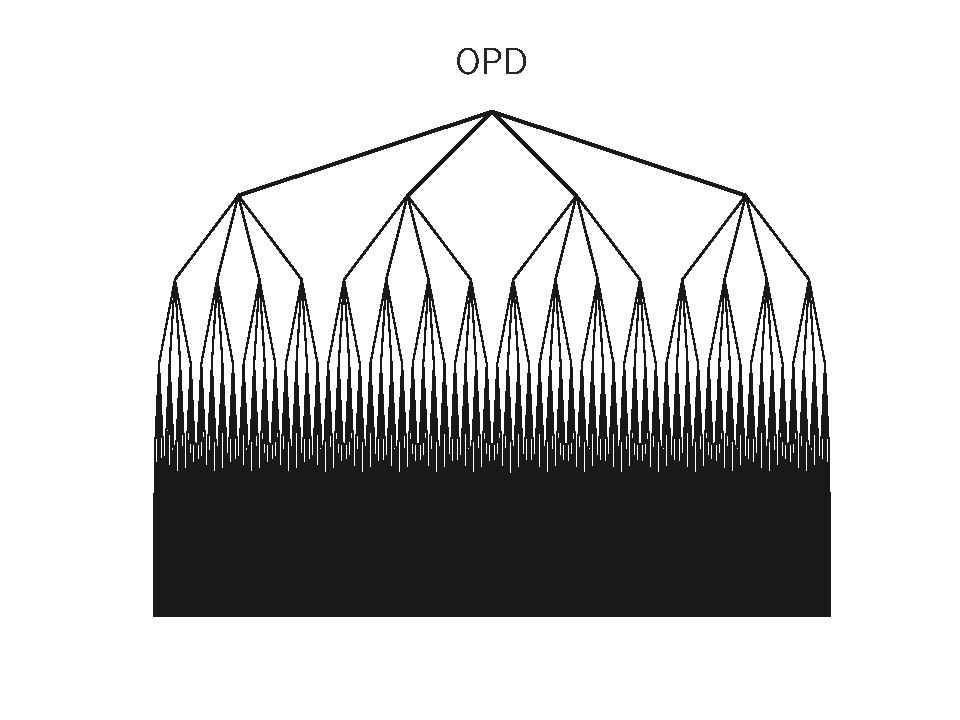
\includegraphics[trim={0 0.5cm 0 0.5cm}, clip, width=0.55\linewidth]{img/gbop/tree_OPD.pdf}
	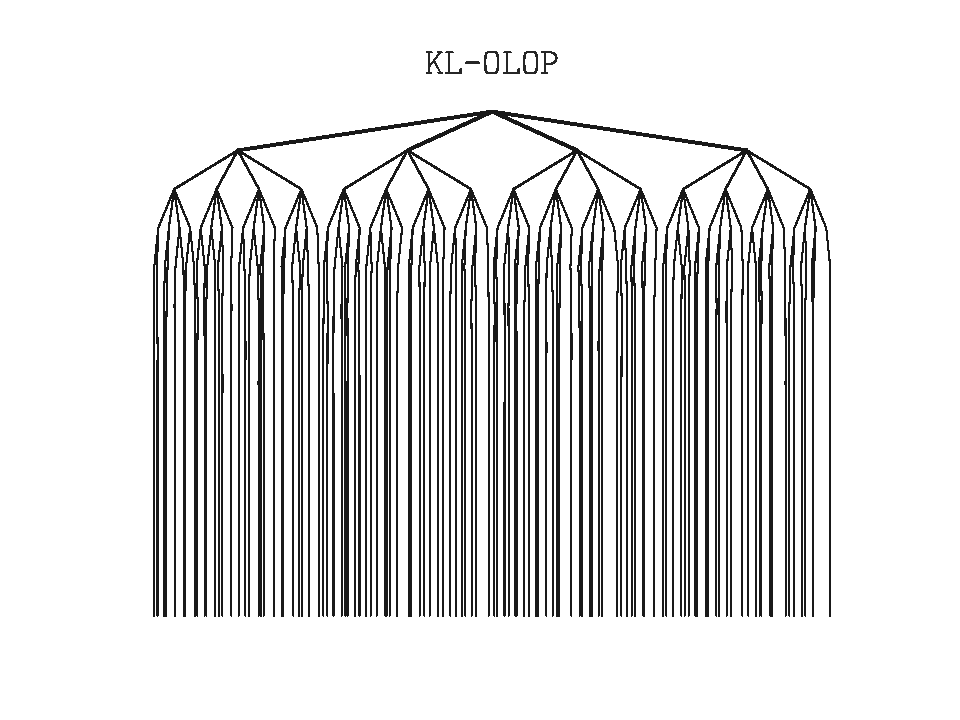
\includegraphics[trim={0 0.5cm 0 0.5cm}, clip, width=0.55\linewidth]{img/gbop/tree_KL-OLOP.pdf}
	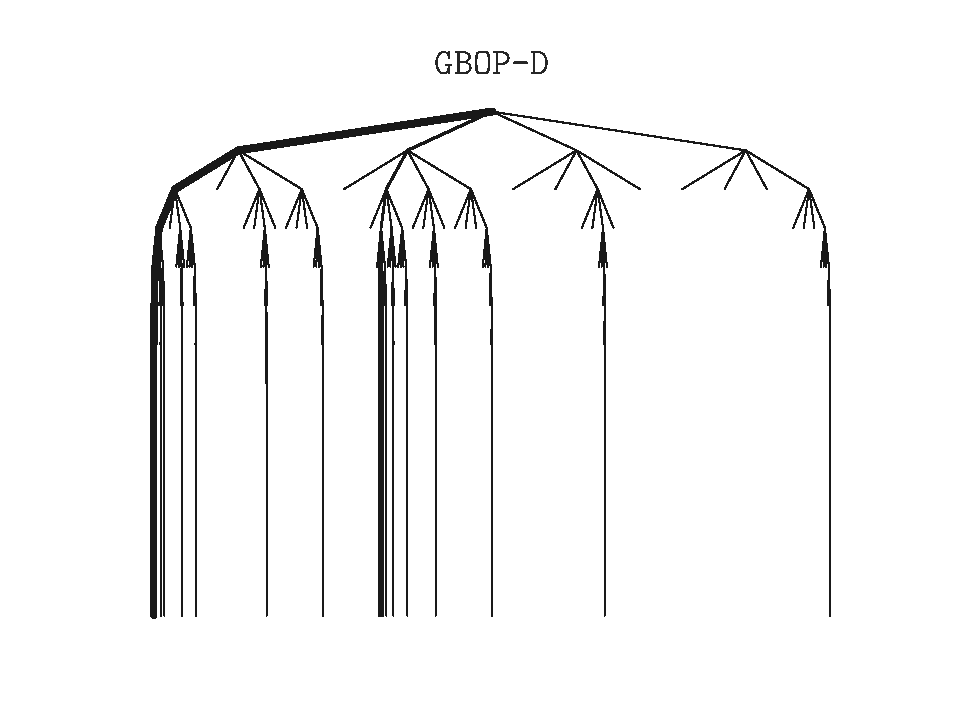
\includegraphics[trim={0 0.5cm 0 0.5cm}, clip, width=0.55\linewidth]{img/gbop/tree_GBOP-D.pdf}
	\caption{Trees expanded by \OPD, by \KLOLOP, and sequences of actions sampled by \GBOPD. The width of edges is proportional to the number of visits.}
	\label{fig:suppl-trees}
\end{figure}

In \Cref{fig:suppl-trees}, we compare the trees $T_n$ expanded by \OPD and \KLOLOP to the unrolled graph $T(\cG_n)$ of \GBOPD in the deterministic gridworld domain. For clarity of the figure, we only display the nodes selected for expansion and not the entire $T(\cG_n)$ as in \Cref{fig:unroll}, since it is infinite and fractal. We observe that \OPD explores uniformly in the space of sequences, which results in a concentrated exploration in the state space as seen in \Cref{fig:deterministic-gridworld}. This phenomenon is similar to the concentration properties of martingales. \KLOLOP behaves similarly, but allocates its bugdet $n$ in fewer trajectories of higher length than \OPD, which results in a sparser tree and slightly better exploration (compare \Cref{fig:deterministic-gridworld} to \Cref{fig:stochastic-gridworld}). In contrast, \GBOPD expands a very sparse and unbalanced tree $T(\cG_n)$ which corresponds to uniform exploration in the state space, and allows to explore deeper for the same budget $n$ (The tree is only shown up to depth $12$, but continues much deeper since the optimal transition is sampled indefinitely once it is discovered). In particular, the paths towards the goal are sampled many times, while other algorithms are still balanced at the root in terms of number of visits.

\section*{Chapter conclusion}

In this chapter, we studied the theoretical and practical performances of planning algorithms.
We first introduced an enhanced version of the \OLOP algorithm for open-loop online planning, whose design was motivated by an investigation of the over-conservative search behaviours of \OLOP. We analysed its sample complexity and showed that the original regret bounds are preserved, while its empirical performances are increased by an order of magnitude in several numerical experiments. Second, we studied the value how merging information between to similar states for planning. We showed that using a graph structure provides a benefit compared to tree structures in the deterministic setting, in the form of an improved regret bound that depends on a smaller problem difficulty. This improvement translates to an enhanced performance in practice, and can be adapted to stochastic problems as we demonstrate experimentally.

\FloatBarrier
\begin{subappendices}
\section{Technical details}

\paragraph{Outline}
We look into the time and memory complexity and propose efficient implementations of \OLOP and \KLOLOP in \Cref{sec:kl-olop-time}, and of \GBOPD and \GBOP in \Cref{gbop-implementation}. We provide proofs for every claimed result about \KLOLOP in \Cref{sec:kl-olop-proofs}, and about \GBOP in \Cref{sec:gbop-proofs}.

\subsection{Time and memory complexity of \KLOLOP}
\label{sec:kl-olop-time}

After having considered the sample efficiency of \OLOP and \KLOLOP in \Cref{thm:regret-kl-olop}, we now study their time and memory complexities. We will only mention the case of \KLOLOP for ease of presentation, but all results easily extend to \OLOP.

The \Cref{algo:kl-olop} requires, at each episode, to compute and store in memory of the reward upper-bounds and U-values of all nodes in the tree $\Tau = \sum_{h=0}^L \cA^h$.
Hence, its time and memory complexities are 
\begin{equation}
C(\KLOLOP) = O(M|\Tau|) = O(MK^L).
\end{equation}

The curse of dimensionality brought by the branching factor $K$ and horizon $L$ makes it intractable in practice to actually run \KLOLOP in its original form even for small problems. However, most of this computation and memory usage is wasted, as with reasonable sample budgets $n$ the vast majority of the tree $\Tau$ will not be actually explored and hence does not hold any valuable information.

We propose in \Cref{algo:lazy-kl-olop} a lazy version of \KLOLOP which only stores and processes the explored subtree, as shown in \Cref{fig:tree}, while preserving the inner workings of the original algorithm.

\begin{figure}[ht]
	\centering
	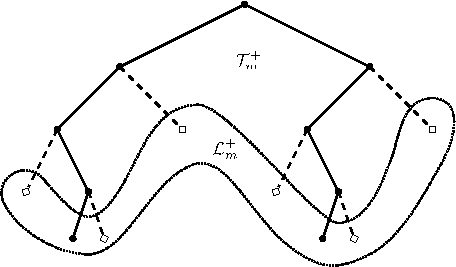
\includegraphics[width=0.6\textwidth]{img/tree_svg-tex}
	\caption{A representation of the tree $\Tau_m^+$, with $K = 2$ actions and after episode $m = 2$, when two sequences have been sampled. They are represented with solid lines and dots \textbullet, and they constitute the explored subtree $\Tau_m$. When extending $\Tau_m$ with the missing children of each node, represented with dashed lines and diamonds $\diamond$, we obtain the full extended subtree $\Tau_m^+$. The set of its leaves is denoted $\LL_m^+$ and shown as a dotted set.}
	\label{fig:tree}
\end{figure}

\begin{algorithm}[tp]
	\DontPrintSemicolon
	Let $M$ be the largest integer such that $M \log M/(2 \log 1/\discount) \leq n$\;
	Let $L = \log M / (2 \log 1/\discount)$\;
	Let $\Tau_0^+ = \LL_0^+ = \{\emptyset\}$\;
	\For{each episode $m = 1, \cdots, M$}{
		Compute $U_a(m-1)$ from \eqref{eq:Ua} for all $a\in\Tau_{m-1}^+$\;
		Compute $B_a(m-1)$ from \eqref{eq:Ba} for all $a\in \LL_{m-1}^+$\;
		Sample a sequence with highest B-value: $a \in \argmax_{a\in \LL_{m-1}^+} B_a(m-1)$\;
		Choose an arbitrary continuation $a^m \in \cA\cA^{L-|a|}$\tcp*{e.g. uniformly}
		Let $\Tau_m^+ = \Tau_{m-1}^+$ and $\LL_m^+ = \LL_{m-1}^+$\;
		\For{$t=1, \cdots, L$}{
			\If{$a^m_{1:t} \not \in \Tau_{m}^+$}{
				Add $a^m_{1:t-1}A$ to $\Tau_{m}^+$ and $\LL_{m}^+$\;
				Remove $a^m_{1:t-1}$ from $\LL_{m}^+$
			}
		}
	}
	\Return the most played sequence $a(n) \in \argmax_{a\in \LL_m^+} N_a(m)$
	\caption{Lazy Open Loop Optimistic Planning}
	\label{algo:lazy-kl-olop}
\end{algorithm}


\begin{proposition}[Time and memory complexity]
	\begin{leftbar}[propositionbar]
		\Cref{algo:lazy-kl-olop} has time and memory complexities of
		\begin{equation*}
		C(\texttt{Lazy KL-OLOP}) = O(KLM^2)
		\end{equation*}
		
		The corresponding complexity gain compared to the original \Cref{algo:kl-olop} is: 
		\begin{equation*}
		\frac{C(\texttt{Lazy KL-OLOP})}{C(\KLOLOP)} = \frac{n}{K^{L-1}}
		\end{equation*}
		which highlights that only a subtree corresponding to the sample budget $n$ is processed instead of the search whole tree $\Tau$.
	\end{leftbar}
\end{proposition}
\begin{proof}
	At episode $m = 1, \cdots, M$, we compute and store in memory the reward upper-bounds and U-values of all nodes in the subtree $\Tau_m^+$. Moreover, the tree $\Tau_m^+$ is constructed iteratively by adding K nodes at most L times at each episode from 0 to $m$. Hence, $|\Tau_m^+| = O(mKL)$.
	This yields directly $C(\texttt{Lazy KL-OLOP}) = \sum_{m=1}^M O(mKL) = O(M^2KL)$.
\end{proof}

\begin{proposition}[Consistency]
	\label{prop:consistency}
	\begin{leftbar}[propositionbar]
		The set of sequences returned by \Cref{algo:lazy-kl-olop} is the same as the one returned by \Cref{algo:kl-olop}.
		In particular, \Cref{algo:lazy-kl-olop} enjoys the same regret bounds as in \Cref{thm:regret}.
	\end{leftbar}
\end{proposition}

\begin{proof}
	To prove consistency of \Cref{algo:lazy-kl-olop}, we need to show that the sequences of actions $a^m$ sampled at every episode are chosen arbitrarily from the same sets as in \Cref{algo:lazy-kl-olop}.
	Namely, 
	
	\begin{equation*}
	\left\{ b\in \cA \cA^{L-|a|} : a \in \argmax_{a\in \LL_{m-1}^+} B_a(m-1)\right\} = \argmax_{a\in \cA^L} B_a(m-1)
	\end{equation*}
	
	To that end, we first introduce some useful notations:
	
	\begin{paragraph}{Definition}
		% We remind that $\Tau$ refers to the whole search tree $\Tau = \sum_{h=0}^L \cA^h$.
		Let $\Tau_m$ be the set of visited nodes after episode $m$:
		\begin{equation*}
		\Tau_m \eqdef \left\{a\in \cA^*: N_a(m) > 0\right\}
		\end{equation*}
		
		We also define its extension $\Tau_m^+$ of visited nodes and their children:
		\begin{equation*}
		\Tau_m^+ \eqdef \Tau_m + \Tau_m A
		\end{equation*}
		
		Now for $a\in \cA^*$, $\pi_m(a)$ (resp. $\pi_m^+(a)$) refers to its longest prefix within $\Tau_m$ (resp. $\Tau_m^+$):
		\begin{align*}
		\pi_m(a) &\eqdef \argmax_{b\in\Tau_m} \{|b|: a\in b \cA^* \} \\
		\pi_m^+(a) &\eqdef \argmax_{b\in\Tau_m^+} \{|b|: a\in b \cA^* \}
		\end{align*}
		
		Finally, $\LL_m$ and $\LL_m^+$ are the image of $\cA^L$ by $\pi_m$ and $\pi_m^+$, respectively.
		\begin{align*}
		\LL_m &\eqdef \pi_m(\cA^L) \\
		\LL_m^+ &\eqdef \pi_m^+(\cA^L) \}
		\end{align*}
	\end{paragraph}
	
	\begin{remark}[About children extensions]
		We could frame \Cref{algo:lazy-kl-olop} in terms of $\Tau_m$ and $\LL_m$, for which mathematical proofs are more straight-forward. However, the iterative construction of $\LL_m$ is tricky and it would require inverting $\pi_m$ on $\LL_m$ which is non-trivial. On the contrary, introducing their extensions  $\Tau_m^+$ and $\LL_m^+$ slightly complicates the proof, but greatly simplifies the construction of $\LL_m^+$ and the computation of ${\pi_m^+}^{-1}$ on $\LL_m^+$, which is why we use these sets in practice.
	\end{remark}
	
	\begin{lemma}[Sets construction]
		$\Tau_m^+$ and $\LL_m^+$ are indeed the sets computed in \Cref{algo:lazy-kl-olop}.
	\end{lemma}
	\begin{proof}
		Note that for each episode $1 \leq m \leq M - 1$, we have:
		\begin{equation}
		\label{eq:tau_mp1}
		\Tau_{m+1} = \Tau_{m} + \sum_{t=0}^L a^{m+1}_{1:t}
		\end{equation}
		Indeed, the nodes visited at least once at time $m+1$ where either already visited once at time $m$ (e.g. in $\Tau_{m}$) or have been visited for the first time during episode $m+1$, which means they are a prefix of $a^{m+1}$. The reverse is clearly true as well.
		
		This enables to write:
		\begin{align*}
		\Tau_{m+1}^+ &= \Tau_{m+1} + \Tau_{m+1}A & \text{by definition}\\
		&= \Tau_{m} + \sum_{t=0}^L a^{m+1}_{1:t} + (\Tau_{m} + \sum_{t=0}^L a^{m+1}_{1:t})A & \text{by \eqref{eq:tau_mp1}} & \\
		&= (\Tau_{m} + \Tau_{m}A) + \sum_{t=0}^L a^{m+1}_{1:t} + \sum_{t=0}^L a^{m+1}_{1:t}A & \\
		&= \Tau_{m}^+ + a^{m+1}_{1:0} + \sum_{t=0}^L a^{m+1}_{1:t}A &\text{ as } \sum_{t=1}^L a^{m+1}_{1:t} \subset \sum_{t=0}^L a^{m+1}_{1:t}A\\
		&=  \Tau_{m}^+ + \sum_{t=0}^L a^{m+1}_{1:t}A  &\text{ as }a^{m+1}_{1:0}=\emptyset \in \Tau_{0} \subset \Tau_{m} \subset \Tau_m^+
		\end{align*}
		This recursion is the one implemented in \Cref{algo:lazy-kl-olop}: at each episode $m$, we add to $\Tau_{m}^+$ the children of the nodes along the sampled action sequence $a^{m}$.
		
		Finally, we highlight that $\LL_m^+ = \pi^+(\cA^L)$ is the set of leaves of $\Tau_{m}^+$.
		Indeed, nodes of $\LL_m^+$ belong to $\Tau_{m}^+$, but they cannot have a child in $\Tau_{m}^+$ as it would contradict the definition of $\LL_m^+$. Conversely, any leaf $a$ of $\Tau_{m}^+$ can be continued arbitrarily to a sequence $b$ of $\cA^L$, which  $a = \pi_m^+(b) \in \pi^+(\cA^L) = \LL_m^+$.
		
		Thus, when updating $\Tau_{m-1}^+$, the set of its leaves is updated accordingly: when the children of a leaf $a^m_{1:t-1}$ are added to $\Tau_m^+$, they become new leaves in place of their parent. Hence, they are added to $\LL_m^+$ while $a^m_{1:t-1}$ is removed from it.
		% 
	\end{proof}
	
	\begin{lemma}[U-values conservation]
		\label{lemma:value-conservation}
		For all $a \in \cA^*$,
		\begin{equation*}
		U_a(m) = U_{\pi_m(a)}(m) = U_{\pi_m^+(a)}(m)
		\end{equation*}
	\end{lemma}
	\begin{proof}
		Let $a \in \cA^*$, denote $h=|a|$ and $h'=|\pi_m(a)|$.
		
		By definition of $\pi_m(a)$, $0 \leq h' \leq h$, and
		\begin{itemize}
			\item for $1\leq t \leq h'$, we have $a_{1:t} = {\pi_m(a)}_{1:t}$ ;
			\item for $h'+1\leq t \leq h$, we have $a_{1:t} \not \in \Tau_m$, hence $T_{a_{1:t}}(m) = 0$ and $U^{\mu}_{a_{1:t}}(m) = 1$.
		\end{itemize}
		Then,
		\begin{align*}
		U_a(m) &= \sum_{t=1}^h \gamma^t U^{\mu}_{a_{1:t}}(m) + \frac{\gamma^{h+1}}{1-\gamma} \\
		&= \sum_{t=1}^{h'} \gamma^t U^{\mu}_{a_{1:t}}(m) + \sum_{t=h'+1}^h \gamma^t \underbrace{U^{\mu}_{a_{1:t}}(m)}_1 + \frac{\gamma^{h+1}}{1-\gamma} \\
		&= \sum_{t=1}^{h'} \gamma^t U^{\mu}_{{\pi_m(a)}_{1:t}}(m) + \frac{\gamma^{h'+1}}{1-\gamma} \\
		&= U_{\pi_m(a)}(m)
		\end{align*}
		
		Now, consider $\pi_m^+(a) \in \Tau_m^+$.
		By definition, it belongs either to $\Tau_m$ or $\Tau_m A$.
		\begin{itemize}
			\item If $\pi_m^+(a) \in \Tau_m$, then $\pi_m^+(a) = \pi_m(a)$ and $U_{\pi_m^+(a)}(m) = U_{\pi_m(a)}(m)$.
			\item Else, $\pi_m^+(a) \in \Tau_m A$ and $p(\pi_m^+(a)) = \pi_m(a)$.
			
			As $\pi_m^+(a) \not \in \Tau_m$, we have $T_{\pi_m^+(a)}(m) = 0$ and $U^{\mu}_{\pi_m^+(a)}(m) = 1$.
			This yields:
			
			\begin{equation*}
			U_{\pi_m^+(a)}(m) = \sum_{t=1}^{h'} \gamma^t U^{\mu}_{{\pi_m^+(a)}_{1:t}}(m) + \gamma^{h'+1} \underbrace{U^{\mu}_{{\pi_m^+(a)}}(m)}_1 + \frac{\gamma^{h'+2}}{1-\gamma} = U_{\pi_m(a)}(m)
			\end{equation*}
			
		\end{itemize}
		We showed that $U_{\pi_m^+(a)}(m) = U_{\pi_m(a)}(m)$, which concludes the proof.
		% 
	\end{proof}
	
	\begin{lemma}[Inverse projection]
		\label{lemma:inverse-proj}
		For all $a\in \LL_m^+$ of length $h\leq L$,
		\begin{equation*}
		{\pi_m^+}^{-1}(a) = a \cA^{L-h}
		\end{equation*}
		
		This allows to easily pick a sequence inside ${\pi_m^+}^{-1}(a)$: just continue the sequence $a$ with a default action of $A$ (e.g. the first) until it reaches length $L$.
	\end{lemma}
	\begin{proof}
		Let $a\in \LL_m^+$. 
		
		By definition of $\pi_m^+$, any sequence in ${\pi_m^+}^{-1}(a)$ is a suffix of $a$ of length $L$, so we clearly have the direct inclusion ${\pi_m^+}^{-1}(a) \subset a \cA^{L-h}$.
		
		Now for the other side: let $b\in \cA \cA^{L-h}$, i.e. $a=b_{1:h}$. We need to show that $\pi_m^+(b) = a$.
		As $a\in \LL_m^+$, there exists $c\in \cA^L$ such that $\pi_m^+(c) = a$.
		\begin{itemize}
			\item If h = L, then $b=a$, so $b \in \LL_m^+ \subset \Tau_m^+$, and hence $\pi_m^+(b)=b=a$.
			\item If h < L, we can show by contradiction that $a \not \in \Tau_m$. Indeed, if $a \in \Tau_m$, then $c_{1:h+1}$ is the child of a node of $\Tau_m$ and hence belongs to $\Tau_m^+$. But then, $c_{1:h+1}$ is a prefix of $c$ in $\Tau_m^+$ with greater length than $a$, which contradicts the definition of $a = \pi_m^+(c)$.
			
			Now, because $a \not \in \Tau_m$, it is also true for all suffixes of $a$, and in particular for $b_{1:t}$ with $h \leq t \leq L$. Indeed, we have $a^s_{1:t} = b_{1:t} \implies a^s_{1:h} = b_{1:h} = a$, so:
			\begin{equation*}
			T_{b_{1:t}}(m) = \sum_{s=1}^m \mathbbm{1}\{a^s_{1:t} = b_{1:t}\} \leq \sum_{s=1}^m \mathbbm{1}\{a^s_{1:h} = a\} = N_a(m) = 0
			\end{equation*}
			Hence, $b_{1:t} \not \in \Tau_m$ for all $h \leq t \leq L$, so in particular $b_{1:t} \not \in \Tau_m^+$ for all $h+1 \leq t \leq L$. Since $b_{1:h} = a \in \Tau_m^+$, $a$ is indeed the longest prefix of $b$ in $\Tau_m^+$, that is: $\pi_m^+(b) = a$.
		\end{itemize}
		We have shown the other side of the inclusion: $a \cA^{L-h} \subset {\pi_m^+}^{-1}(a)$, which entails that the two sets are in fact equal.
		% 
	\end{proof}
	
	We can now conclude our proof of \Cref{prop:consistency}: at episode $m$, \KLOLOP samples a sequence of action $a^m$ within the set $\argmax_{a\in \cA^L} U_a(m)$. 
	However, we have:
	
	\begin{align*}
	\argmax_{c\in \cA^L} U_c(m) &= \argmax_{c\in \cA^L} U_{\pi_m^+(c)}(m) & \text{by \Cref{lemma:value-conservation}} \\
	&= {\pi_m^+}^{-1}\left(\argmax_{a\in {\pi_m^+}(\cA^L)} U_{a}(m)\right) & \\
	&= \left\{b\in{\pi_m^+}^{-1}(a) : a\in \argmax_{a\in \LL_m^+} U_{a}(m)\right\} & \\
	&= \left\{b\in \cA \cA^{L-|a|} : a\in \argmax_{a\in \LL_m^+} U_{a}(m)\right\} & \text{by \Cref{lemma:inverse-proj}} 
	\end{align*}
	
	Thus, at each episode the sequence of actions $a^m$ sampled by \Cref{algo:lazy-kl-olop} could have been sampled by \Cref{algo:kl-olop} as well.
	
	In particular, if the arbitrary rule used to pick a sequence from a set is the same for the two algorithms, then the sampled sequences $a^m$ will be identical, will have the same visit count $T_{a^m}(m)$, and in the end the returned action $a(n)$ will be the same.
	% 
\end{proof}

\subsection{Time and memory complexity of \GBOP}
\label{sec:gbop-implementation}

In this section, we provide more details about the implementation of \GBOPD and \GBOP. First, we discuss how two procedures can be approximated so that they terminate in finite time, and study the impact of this approximation on the regret guarantees. Second, we propose a lazy implementation of the bounds computation through $\cB_n^\infty$ that only considers a subset of nodes to update.

\subsubsection{Termination}

\paragraph{Bounds computation}

The bounds computation step $\cB_n^\infty$ (line 1 of \GBOPD) can converge in infinite time whenever $\cG_n$ contains a loop, as shown in \Cref{fig:simple_loop}. We consider the effect of stopping early after a fixed number of iterations $k(\varepsilon,\gamma)$.

\begin{figure}[th]
	\centering
	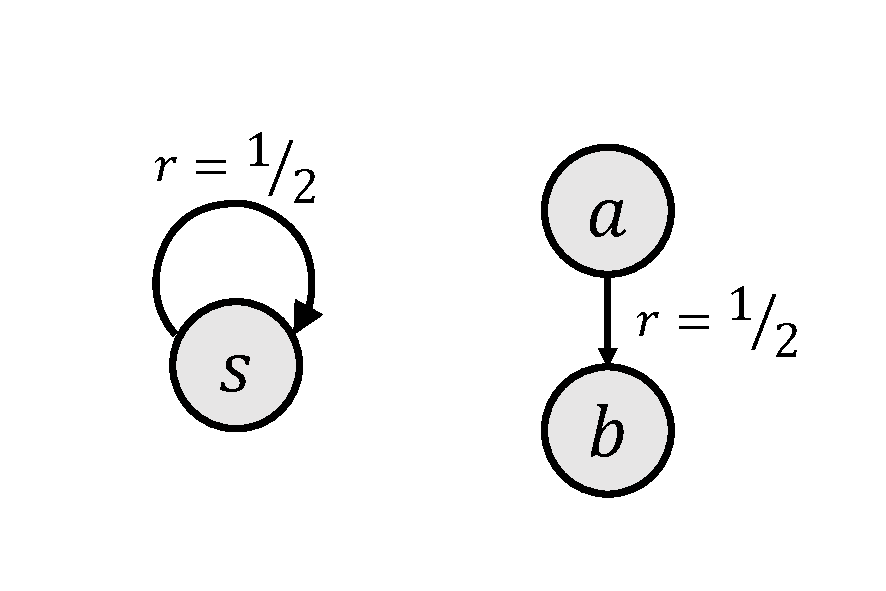
\includegraphics[trim=2.5cm 1cm 9cm 2cm, clip, width=0.1\linewidth]{img/gbop/loop.pdf}\\
	\begin{tabular}{lccccc}
		\toprule
		$k$ & $0$ & $1$ & $\cdots$ & $k$ \\
		\midrule
		$\cU = \cB^k(V_{\max})(s)$ & $V_{\max}$ & $\frac{1}{2} + \gamma V_{\max}$ && $\frac{1}{2}(1-\gamma^k)V_{\max} + \gamma^k V_{\max}$\\
		$\cL = \cB^k(0)(s)$ & $0$ & $\frac{1}{2}$ && $\frac{1}{2}(1-\gamma^k)V_{\max}$\\
		\bottomrule
	\end{tabular}
	\caption{\textbf{Top}: a simple looping MDP with $|S|=|A|=1$ after having observed a single transition ($n=1$). \textbf{Bottom}: the sequence of bounds $\cB_1^k(0)$ and $\cB_1^k(V_{\max})$. They converge geometrically to their limit $\cU_1 = \cL_1 = V = \frac{1}{2}V_{\max}$, thus in infinite time.}
	\label{fig:simple_loop}
\end{figure}

\begin{proposition}[Time complexity of bounds computation]
	An $\varepsilon$-approximation of $(\cL_n, \cU_n)$ can be computed by applying $\cB_n$ for a finite number $k(\epsilon,\gamma)$ of iterations, with $$k(\epsilon,\gamma) = \log_\gamma\frac{1}{\varepsilon(1-\gamma)}.$$ 
\end{proposition}
\begin{proof}
	$\cB_n$ is a $\gamma$-contraction by Lemma \ref{lem:properties-b-graph}, and $\cU_n$ (resp $\cL_n$) is at a distance (in $\|\dot\|_\infty$) at most $V_{\max}$ of the initial value bound $V_{\max}$ (resp $0$). Thus, the $k^{\text{th}}$ application of $\cB_n$ decreases this error by a factor $\gamma^k$, which gives the result.
	\end{proof}

The impact of using an $\varepsilon$-approximation of $(\cL_n, \cU_n)$ during planning is the following:
\begin{proposition}[Effect of early stopping]
	\label{prop:early-stopping}
	Denote the approximate bounds $(\hat{\cL}_n, \hat{\cU}_n)$ obtained by applying $\cB_n^{k(\varepsilon,\gamma)}$ instead of $\cB_n^\infty$, and likewise $(\hat{L}_n, \hat{U}_n)$ in their tree version obtained by applying $B_n^{k(\varepsilon,\gamma)}$ instead of $B_n^\infty$.
	Then, running \GBOPD with $\hat{\cL}_n, \hat{\cU}_n$ gives the following regret:
	\begin{align*}
	\regret = \tilde{\cO}\left(n^{-\log \frac{1}{\gamma}/\hlob{\log \hat{\kappa}_\infty}}\right),
	\end{align*}
	with $$\hlgb{{\kappa}_\infty} \leq \hlob{\hat{\kappa}_\infty \eqdef \lim_{n\rightarrow\infty} \kappa(\hat{L}_n, \hat{U}_n)} \leq \hlrb{\kappa}.$$
	Moreover, the approximation gap $\hlgb{\kappa_\infty} - \hlob{\hat{\kappa}_\infty}$ is non-increasing with respect to $\varepsilon$.
\end{proposition}
It is difficult to control more explicitly the gap between $\hlgb{\kappa_\infty}$ and $\hlob{\hat{\kappa}_\infty}$, which might be discontinuous with $\varepsilon$.

\begin{proof}
	Note that $\hat{L}_n$ and $\hat{U}_n$ are valid monotonic bounds on $V$, verifying
	\[0\leq \hat{L}_n\leq {L}_n \leq V \leq {U}_n\leq \hat{U}_n \leq V_{\max}.\]
	Thus, Lemma \ref{lem:bounds} holds with the difference that we only have an inequality $$\overline{U_n}(a) \geq \max_{a'\in a \cA^\infty} \overline{U}(a')$$ rather than an equality, by monotonicity but non-invariance by $B_n$. However, this was the actual inequality used in Lemma \ref{lem:expansion-bound}, which still holds by replacing $L_n,U_n$ by their approximation $\hat{L}_n,\hat{U}_n$. Likewise, Lemma \ref{lem:recommendation-bound} holds. The proof of \Cref{thm:regret-gbop}, can be written with the modification that expanded nodes belong to $T_h^\infty(\hat{L}_n, \hat{U}_n))$, which gives the claimed bound.
	
	As $\varepsilon$ decreases, $k(\epsilon,\gamma)$ increases, which means by Lemma \ref{lem:properties-b-tree} that $(\hat{\cL}_n, \hat{\cU}_n)$ get tighter and $\hlob{\hat{\kappa}_\infty}$ shrinks by Lemma \ref{lem:shrink}. It reaches its minimum $\hlgb{\kappa_\infty}$ when $\varepsilon=0$.
	\end{proof}

Thus, we observe that there is a \emph{tradeoff} between the time complexity $k(\varepsilon)$ and the sample complexity $\hlob{\hat{\kappa}_\infty}$: decreasing one increases the other.

Note that \OPD uses $d_n$ iterations of $B_n$, which corresponds to a tuning of $\varepsilon$ with $n$: $\varepsilon_n = \frac{\gamma^{d_n}}{1-\gamma} = \cO(n^{-\frac{\log 1/\gamma}{\log \kappa}})$. 


\paragraph{Sampling rule}

The sampling rule of \GBOPD (line 2 of \GBOPD) can yield an infinite sequence $b_n$. We propose to stop the sampling after a fixed depth $d^+_n$.

\begin{proposition}[Time complexity of sampling]
	Consider the variant of \GBOPD where we stop the sampling rule when reaching a fixed depth $d^+_n$ chosen polynomial with $n$:
	\[d^+_n = \ceil{\alpha n^\beta},\; \text{with }\alpha,\beta > 0\]
	Then, the regret bound of \Cref{thm:regret-gbop} (or that of Proposition \ref{prop:early-stopping} when using early stopping in the bounds computation) still holds.
\end{proposition}

Note that this is not too constraining compared to \OPD, for which the sampling rule complexity $d_n$ is upper-bounded by $n$. Hence, by choosing $\alpha=\beta=1$, \GBOPD preserve the same complexity as \OPD in the worst case.

\begin{proof}
	Let $\kappa'>\hlgb{{\kappa}_\infty}$ (or $\kappa'>\hlob{\hat{\kappa}_\infty}$ under approximate bounds). In the proof of \Cref{thm:regret-gbop}, it is shown that the maximum depth $d_n$ of an expanded node is at least $d^-_n \eqdef \log_{\kappa'}\frac{n-C_0}{C_1'}$, which allows to conclude with Lemma \ref{lem:recommendation-bound} that $\regret = \cO(\gamma^{d_n}) = \cO(\gamma^{d^-_n})$. By choosing $d^+_n$ polynomial, we have that $d^+_n$ is greater than $d^-_n$ for $n$ sufficiently high. Thus, by stopping the sampling after reaching a depth $d^+_n$, we have that $\regret \leq \gamma^{\min\{d_n, d^+_n\}} / (1-\gamma) = \cO(\gamma^{d^-_n}) = \cO(n^{\frac{-\log 1/\gamma}{\log \kappa'}})$
	\end{proof}

\subsubsection{Efficient implementation of $\cB_n^\infty$}

The bounds $\cL_n$ and $\cU_n$ are computed by fixed-point iteration of $\cB_n$ from the trivial bounds $(0,V_{\max})$. The naive implementation of $\cB_n$ requires to iterate over the whole set of state-action pairs in $\cG_n$. 
Two ideas can be used to increase the efficiency of both steps:
\begin{enumerate}[label=(\roman*)]
	\item Instead of starting the iteration with the trivial bounds, the previous estimate $\cL_{n-1}, \cU_{n-1}$ can be used instead at iteration $n$. Since these bounds are closer to their limit ($0\leq \cL_{n-1}\leq \cL_n$ and $\cU_n\leq \cU_{n-1} \leq V_{\max}$), the fixed-point iteration will converge quicker.
	\item In particular, since $\cL_{n-1}$ and $\cU_{n-1}$ are invariant by $\cB_n$, the the only nodes modified by a supplementary application of $\cB_n$ are the parents of only updated node: the expanded state $s_n$. Once its value is updated by $\cB_n$, the same reasoning can be applied for the next iteration of $\cB_n$: only its predecessors can be updated. Thus, we can keep track of a set $q$ of states that can be updated, for every application of $\cB_n$.
\end{enumerate}
These idea are formalised in \Cref{alg:queue-b-inf}. Note that the criterion $\|\cB_n^{k+1} - \cB_n^k\| \leq \frac{1-\gamma}{\gamma}\varepsilon$ is used to detect that the limit $\cB_n^\infty$ is approximated with accuracy $\varepsilon$, and stems from $\cB_n$ being a $\gamma$-contraction:
\begin{proof}
	$\|\cB_n^k - \cB_n^\infty\| \leq \gamma\| \cB_n^{k+1} - \cB_n^\infty\| \leq \gamma \|\cB_n^{k+1} - \cB_n^{k}\| + \gamma \|\cB_n^{k} - \cB_n^\infty\|$, with $\| \cB_n^{k+1} - \cB_n^{k}\| \leq \frac{1-\gamma}{\gamma}\varepsilon$, thus $\|\cB_n^{k} - \cB_n^\infty\| \leq \varepsilon$.
	\end{proof}

\begin{algorithm}
	\caption{A queue-based implementation of $\cB_n^\infty$.}
	\label{alg:queue-b-inf}
	\KwIn{Initial bound $\cU_{n-1}$, expanded node $s_n$, accuracy $\varepsilon$}
	\KwOut{An $\varepsilon$-approximation of $\cU_{n}$}
	\DontPrintSemicolon
	$\cU_n \gets \cU_{n-1}$\;
	$q\gets [s_n]$\;
	\While{$q$ is not empty}{
		$s'\gets$ Pop the first node from the queue $q$\;
		$\cU' \gets \cB_n(\cU_n)(s')$\Comment*[r]{Node backup}
		\If(\Comment*[f]{Stopping rule}){$\cU' - \cU_n > \frac{1-\gamma}{\gamma}\varepsilon$}{
			Push the predecessors $s$ of $s'$ to the queue $q$ \Comment*[r]{Propagation rule}
		}
		$\cU_n(s') \gets \cU'$\;
	}
	\Return $\cU_n$\;
\end{algorithm}


\subsection{Proofs of \KLOLOP results}
\label{sec:kl-olop-proofs}

\subsubsection{Proof of \Cref{lemma:expected-regret}}
\begin{proof}
	The proof is identical to that of Lemma 4 in \citep{Bubeck2010}.
	
	Since $\arg \max _{a \in \cA} T_{a}(M)$, and $\sum_{a \in \cA} T_{a}(M)=M,$ we have $T_{a(n)}(M) \geq M / K$, and thus:
	\begin{equation*}
	\frac{M}{K}(V-V(a(n))) \leq(V-V(a(n))) T_{a(n)}(M) \leq \sum_{m=1}^{M} V-V\left(a^{m}\right)
	\end{equation*}
	Hence, we have, $r_{n} \leq \frac{K}{M} \sum_{m=1}^{M} V-V\left(a^{m}\right)$. Now remark that, for any sequence of actions $a\in \cA^L$, we have either:
	\begin{itemize}
		\item $a_{1 : H} \in \mathcal{I}_{H} ;$ which implies $V-V(a) \leq \frac{2 \gamma^{H+1}}{1-\gamma}$
		\item or there exists $1\leq h \leq H$ such that $a_{1:h} \in \mathcal{J}_h$; which implies $V-V(a) \leq V-V\left(a_{1 : h-1}\right)+\frac{\gamma^{h}}{1-\gamma} \leq \frac{3 \gamma^{h}}{1-\gamma}$.
	\end{itemize}
	Thus we can write:
	\begin{equation*}
	\begin{aligned} \sum_{m=1}^{M}\left(V-V\left(a^{m}\right)\right) &=\sum_{m=1}^{M}\left(V-V\left(a^{m}\right)\right)\left(\mathbbm{1}\left\{a^{m} \in \mathcal{I}_{H}\right\}+\mathbbm{1}\left\{\exists 1 \leq h \leq H : a_{1 : h}^{m} \in \mathcal{J}_{h}\right\}\right) \\ & \leq \frac{2 \gamma^{H+1}}{1-\gamma} M+3 \sum_{h=1}^{H} \sum_{a \in \mathcal{J}_{h}} \frac{\gamma^{h}}{1-\gamma} T_{a}(M) \end{aligned}
	\end{equation*}
	
\end{proof}

\subsubsection{Proof of \Cref{lemma:size_Ph}}
\begin{proof}
	The event $\tau^a_{h,h'}=1$ implies $a^{m+1}\in a A^*$ and \eqref{eq:sampled-enough}. This implies by \Cref{lemma:sub-optimal-pull} that either \eqref{eq:cond-ukl}, \eqref{eq:cond-lkl} or \eqref{eq:cond-dkl} is satisfied. Now by \Cref{lemma:ci-length} this implies that either \eqref{eq:cond-ukl} is true or \eqref{eq:cond-lkl} is true or \eqref{eq:sampled-enough-h} is false. We now prove that if \eqref{eq:P-min-size} is not satisfied then \eqref{eq:sampled-enough} is true, which clearly ends the proof.
	This follows from: For any $0 \leq t \leq h'$:
	
	\begin{align*}
	T_{a_{1:t}}(m) &= \sum_{b\in a_{1:t}A^{h-t}} T_b(m) \geq \sum_{b\in \mathcal{P}^{a_{1:t}}_{h,h'}} T_b(m) \\
	&\geq \left(\gamma^{2(t-h')}\right) \left(2f(m)(h+1)^2\gamma^{2(h'-h-1)}\right)\\
	&= 2f(m)(h+1)^2\gamma^{2(t-h-1)}\,.\qquad\qquad
	\end{align*}
	%\
\end{proof}

\subsubsection{Proof of \Cref{lemma:expected-P-size}}

\begin{proof}
	The proof is identical to that of Lemma 9 in \citep{Bubeck2010}.
	
	\noindent
	Let $h'\geq 1$ and $0 \leq s \leq h'$. We introduce the following random variables:
	\begin{equation*}
	m_{s}^{a}=\min \left(M, \min \left\{m \geq 0 :\left|\mathcal{P}_{h, h^{\prime}}^{a}(m)\right| \geq \gamma^{2\left(s-h^{\prime}\right)}\right\}\right).
	\end{equation*}
	We will prove recursively that,
	\begin{equation}
	\label{eq:toprove}
	\left|\mathcal{P}_{h, h^{\prime}}^{\emptyset}(m)\right| \leq \sum_{t=0}^{s} \gamma^{2\left(t-h^{\prime}\right)}\left|\mathcal{I}_{t}\right|+\sum_{a \in \mathcal{I}_{s}}\left|\mathcal{P}_{h, h^{\prime}}^{a} \setminus \cup_{t=0}^{s} \mathcal{P}_{h, h^{\prime}}^{a_{1:t}}\left(m_{t}^{a_{1:t}}\right)\right|
	\end{equation}
	The result is true for $s = 0$ since $\mathcal{I}_0 = \{\emptyset\}$ and by definition of $m^\emptyset_0$,
	\begin{equation*}
	\left|\mathcal{P}_{h, h^{\prime}}^{\emptyset}(m)\right| \leq \gamma^{-2 h^{\prime}}+\left|\mathcal{P}_{h, h^{\prime}}^{\emptyset}(m) \setminus \mathcal{P}_{h, h^{\prime}}^{\emptyset}\left(m_{0}^{\emptyset}\right)\right|
	\end{equation*}
	Now let us assume that the result is true for $s<h'$. We have:
	\begin{align*}
	\sum_{a \in \mathcal{I}_{s}}\left|\mathcal{P}_{h, h^{\prime}}^{a}(m) \setminus \cup_{h, h^{\prime}}^{a_{1 : t}}\left(m_{t}^{a_{1 : t}}\right)\right|&=\sum_{a \in \mathcal{I}_{s+1}}\left|\mathcal{P}_{h, h^{\prime}}^{a}(m) \setminus \cup_{t=0}^{s} \mathcal{P}_{h, h^{\prime}}^{a_{1 : t}}\left(m_{t}^{a_{1 : t}}\right)\right|\\
	&\leq \sum_{a \in \mathcal{I}_{s+1}} \gamma^{2\left(s+1-h^{\prime}\right)}+\left|\mathcal{P}_{h, h^{\prime}}^{a}(m) \setminus \cup_{t=0}^{s+1} \mathcal{P}_{h, h^{\prime}}^{a_{1 : t}}\left(m_{t}^{a_{1 : t}}\right)\right|\\
	&= \gamma^{2\left(s+1-h^{\prime}\right)}\left|\mathcal{I}_{s+1}\right|+\sum_{a \in \mathcal{I}_{s+1}}\left|\mathcal{P}_{h, h^{\prime}}^{a}(m) \setminus \cup_{t=0}^{s+1} \mathcal{P}_{h, h^{\prime}}^{a_{1 ; t}}\left(m_{t}^{a_{1 : t}}\right)\right|
	\end{align*}
	which ends the proof of \eqref{eq:toprove}. Thus we proved (by taking $s=h'$ and $m=M$):
	\begin{equation*}
	\begin{aligned}\left|\mathcal{P}_{h, h^{\prime}}^{\emptyset}(M)\right| & \leq \sum_{t=0}^{h^{\prime}} \gamma^{2\left(t-h^{\prime}\right)}\left|\mathcal{I}_{t}\right|+\sum_{a \in \mathcal{I}_{h^{\prime}}}\left|\mathcal{P}_{h, h^{\prime}}^{a}(M) \setminus \cup_{t=0}^{s+1} \mathcal{P}_{h, h^{\prime}}^{a_{1 : t}}\left(m_{t}^{a_{1 : t}}\right)\right.\\ &=\sum_{t=0}^{h^{\prime}} \gamma^{2\left(t-h^{\prime}\right)}\left|\mathcal{I}_{t}\right|+\sum_{a \in \mathcal{J}_{h}}\left|\mathcal{P}_{h, h^{\prime}}^{a}(M) \setminus \cup_{h, h^{\prime}}^{a_{1 : t}}\left(m_{t}^{a_{1 : t}}\right)\right| \end{aligned}
	\end{equation*}
	
	Now, for any $a\in \mathcal{J}_h$, let $\tilde{m} = \max_{0\leq t\leq h'} m_t^{a_{1:t}}$. Note that for $m\geq \tilde{m}$, equation \eqref{eq:P-min-size} is not satisfied. Thus we have
	\begin{equation*}
	\begin{aligned}
	\left|\mathcal{P}_{h, h^{\prime}}^{a} \setminus \cup_{h, h^{\prime}}^{s+1} \mathcal{P}_{h, h^{\prime}}^{a_{1 : t}}\left(m_{t}^{a_{1 : t}}\right)\right|=&\sum_{m=\tilde{m}}^{M-1} \tau_{h, h^{\prime}}^{a}(m+1)=\sum_{m=0}^{M-1} \tau_{h, h^{\prime}}^{a}(m+1) \mathbbm{1}\{\eqref{eq:P-min-size} \text { is not satisfied }\} \\ & \leq \sum_{m=0}^{M-1} \tau_{h, h^{\prime}}^{a}(m+1) \mathbbm{1}\{\eqref{eq:cond-ukl} \text { or }\eqref{eq:cond-lkl}\} \end{aligned}
	\end{equation*}
	where the last inequality results from \Cref{lemma:size_Ph}. Hence, we proved:
	
	\begin{equation*}
	\left|\mathcal{P}_{h, h^{\prime}}^{\emptyset}\right| \leq \sum_{t=0}^{h^{\prime}} \gamma^{2\left(t-h^{\prime}\right)}\left|\mathcal{I}_{t}\right|+\sum_{m=0}^{M-1} \sum_{a \in \mathcal{J}_{h}} \mathbbm{1}\{\eqref{eq:cond-ukl}\text{ or }\eqref{eq:cond-lkl}\}
	\end{equation*}
	
	Taking the expectation and applying \Cref{lemma:boundary-crossing-prob} yield the claimed bound for $h'\geq 1$.
	
	Now for $h' = 0$ we need a modified version of \Cref{lemma:size_Ph}. Indeed in this case one can directly prove that $\tau_{h,0}^a(m+1)=1$ implies that either equation \eqref{eq:cond-ukl} or \eqref{eq:cond-lkl} is satisfied (this follows from the fact that $\tau_{h,0}^a(m+1)=1$ always imply that \eqref{eq:sampled-enough-h} is true for $h'= 0$). Thus we obtain:
	\begin{equation*}
	\left|\mathcal{P}_{h, h^{\prime}}^{\emptyset}\right|=\sum_{m=0}^{M-1} \sum_{a \in \mathcal{J}_{h}} \tau_{h, 0}^{a}(m+1) \leq \sum_{m=0}^{M-1} \sum_{a \in \mathcal{J}_{h}} \mathbbm{1}\{\eqref{eq:cond-ukl}\text{ or }\eqref{eq:cond-lkl}\}
	\end{equation*}
	Taking the expectation and applying \Cref{lemma:boundary-crossing-prob} yield the claimed bound for $h' = 0$ and ends the proof.
	
\end{proof}

\subsubsection{Proof of \Cref{lemma:expected-plays-count}}

\begin{proof}
	The proof is identical to that of Lemma 10 in \citep{Bubeck2010}:
	\begin{align*}
	\sum_{a \in \mathcal{J}_{h}} T_{a}(M) = {} & \sum_{a \in \mathcal{J}_{h} \backslash \mathcal{P}_{h, h-1}^{\emptyset}} T_{a}(M)+\sum_{h^{\prime}=1}^{h-1} \sum_{a \in \mathcal{P}_{h, h^{\prime}}^{\emptyset} \setminus \mathcal{P}_{h, h^{\prime}-1}^{\emptyset}} T_{a}(M)+\sum_{a \in \mathcal{P}_{h, 0}^{\emptyset}} T_{a}(M)\\
	\leq {} & 2f(m)(h+1)^{2} \gamma^{2(h-2-h)}\left|\mathcal{J}_{h}\right| \\
	 &+ \sum_{h^{\prime}=1}^{h-1} 2f(m)(h+1)^{2} \gamma^{2\left(h^{\prime}-2-h\right)} \log M\left|\mathcal{P}_{h, h^{\prime}}^{\emptyset}\right|+M\left|\mathcal{P}_{h, 0}^{\emptyset}\right|\\
	= {} &\tilde{O}\left(\left(\kappa^{\prime}\right)^{h}+\gamma^{-2 h} \sum_{h^{\prime}=1}^{h-1} \gamma^{2 h^{\prime}}\left|\mathcal{P}_{h, h^{\prime}}^{\emptyset}\right|+M\left|\mathcal{P}_{h, 0}^{\emptyset}\right|\right)
	\end{align*}
	Taking the expectation and applying the bound of \Cref{lemma:expected-P-size} give the claimed bound.
	
\end{proof}


\subsection{Proof of \GBOP results}
\label{sec:gbop-proofs}

\subsubsection{Proof of Lemma \ref{lem:properties-b-tree}}
\begin{proof}
The tightening property is directly obtained by definition of monotonicity.
Let us show the preservation of monotonicity. Let $U$ a monotonic upper-bound, $a\in \cA^h$. Then, for any $b\in \cA$:
\begin{align*}
U(ab) \geq B(U)(ab) \implies 
r(ab) + \gamma U(ab) \geq r(ab) + \gamma B(U)(ab).
\end{align*}
Thus, my taking the $\max$ on $b$,
$
B(U)(a) \geq B^2(U)(a).
$
The same can be obtained for a lower-bound $L$.

The finite time convergence can be obtained by recursion from the leaves to the root, by noticing that if the value of a set of siblings $aA$ is invariant by $B$, then the value of their parent $a$ is invariant by $B^2$.
\end{proof}

\subsubsection{Proof of \Cref{lem:properties-b-graph}}
\begin{proof}
The proof of tightening and monotonicity preservation is the same as that of Lemma \ref{lem:properties-b-tree}.
The contraction property is standard for the Bellman Operator, see e.g. Puterman M., Markov Decision Processes: Discrete Stochastic Dynamic Programming (2005).
\end{proof}

\subsubsection{Proof of \Cref{thm:regret-opd}}
We recall the main steps of the proof of \citet{Hren2008optimistic}.\\

\begin{enumerate}
	\item The recommendation $a_n$ has a maximal depth $d_n$ in the tree, and its gap $\regret = V^\star - V({a_{n,1}})$ is bounded by $\regret \leq \frac{\gamma^{d_n}}{1-\gamma}$. We need to relate $d_n$ to $n$.
	
	\item Each expanded node belongs to $\Tau^\infty = \bigcup_{h\geq 0} \Tau_h^\infty$, where $$\Tau_h^\infty = \left\{a\in \cA^h: V^\star-V(a) \leq \frac{\gamma^h}{1-\gamma}\right\}.$$ Introduce the difficulty measure $\kappa$ such that $|\Tau_h^\infty| = \cO(\kappa^h)$ (the smallest).
	
	\item In the worst case, expanded nodes fully fill the depths of $\Tau^\infty$ up to $d_n$: $n = \sum_{d=1}^{d_n} n_d \leq  C\sum_{d=1}^{d_n} \kappa^d = \begin{cases}
	\cO(d_n) &\text{if $\kappa=1$}\\
	\cO(\kappa^{d_n}) &\text{else.}
	\end{cases}$\\
	Hence $\regret = \begin{cases}
	\cO(\gamma^n) &\text{if $\kappa=1$}\\
	\cO(\gamma^{\frac{\log n}{\log \kappa}}) = \cO(n^{-\frac{\log 1/\gamma}{\log \kappa}}) &\text{else.}
	\end{cases}$
\end{enumerate}

\subsubsection{Proof of \Cref{lem:shrink}}

\begin{proof}
Let $L_2\leq L_1\leq V\leq U_1\leq U_2$, then $\Tau_h^\infty(L_1,U_1) \subset \Tau_h^\infty(L_2,U_2),$ which implies $$|\Tau_h^\infty(L_1,U_1)|^{1/h} \leq |\Tau_h^\infty(L_2,U_2)|^{1/h}$$ and the claimed result in the limit $h\rightarrow\infty$.
\end{proof}

\subsubsection{Proof of \Cref{thm:regret-bound-U}}
In this proof, we temporarily assume that $U=B(U)$ and $L=B(L)$. We follow the same steps as in the proof of the regret of \texttt{OPD}.

\begin{remark}
It no longer holds that $a_n$ must be of maximal depth $d_n$.  This is due to the fact the exploration bonus $\gamma^h U(a)$ is not depth-wise constant: consider two nodes $a,b$ at the same depth with $R(a) > R(b)$. In \texttt{OPD}, both get the same bonus $\gamma^h/(1-\gamma)$, and the node $a$ is expanded first. But with the local bonus, $b$ could be expanded in priority rather than $a$, if its own bonus is sufficiently higher than that of $a$, precisely if $R(a)+\gamma^h U(a) < R(b)+\gamma^h U(b)$. For instance, $U(a)=0$ when $a$ is known to be a terminal state while $b$ can lead to future rewards. If after expanding and exploring the subtree of $b$ we find out that $V(b) = 0$, we still return the recommendation $a$, which is of non-maximal depth.
\end{remark}

The regret bound still holds, however. First, notice that:
\begin{lemma}[Expansion]
\label{lem:expansion-bound-U}
Whenever a node $a$ of depth $h$ is expanded by the optimistic algorithm, its first action $a_1$ enjoys a simple regret $V(a^\star)-V(a_1) \leq \gamma^h(U(a)-L(a))$. 
\end{lemma}
\begin{proof}
Let $t$ be the time of expansion of $a$, it holds that $\overline{U}_t(b) \leq \overline{U}_t(a)$ for all $b\in \ext{\Tau}_t$, in particular those in a branch starting by an optimal action $a^\star$. Since $U=B(U)$ and $L=B(L)$, we also have $\overline{U}_t(a^\star) = \max_{b\in a^\star A^*} \overline{U}_t(b) \leq \overline{U}_t(a)$, and $\overline{L}_t(a_1) = \max{b\in a_1 A^*} \overline{L}_t(b) \geq  \overline{L}_t(a)$. Thus, $V(a^\star)-V(a_1) \leq \overline{U}_t(a^\star) - \overline{L}_t(a_1) \leq \overline{U}_t(a) - \overline{L}_t(a) = \gamma^h(U(a)-L(a))$.
\end{proof}
 
\begin{lemma}[Recommendation]
	\label{lem:recommendation-bound-U}
The recommended action $a_n$ has a simple regret $\regret \leq \frac{\gamma^{d_n}}{1-\gamma}$, where $d_n$ is the maximal depth of $\Tau_n$.
\end{lemma}
\begin{proof}
Let $i$ a node of maximal depth $d_n$, and consider the recommended node $a_n$ at time $n$, of depth $d$. In particular, $\overline{L}_n(a_n) \geq \overline{L}_n(i)$, and since $(\overline{L}_t)_t$ is non-decreasing we also have $\overline{L}_n(i) \geq \overline{L}_t(i)$. At the time $t$ when $i$ is expanded, we have $\overline{U}_t(a_n) \leq \overline{U}_t(i)$, and since $(\overline{U}_t)_t$ is non-increasing we also have $\overline{U}_n(a_n) \leq \overline{U}_t(a_n)$. We can conclude with Lemma \ref{lem:expansion-bound-U} applied to $a_n$: $\regret \leq \gamma^d(U(a_n)-L(a_n) = \overline{U}_n(a_n) - \overline{L}_n(a_n)  \leq \overline{U}_t(a_n) - \overline{L}_n(i) \leq \overline{U}_t(i) - \overline{L}_t(i) = \gamma^{d_n}(U(i) - L(i)$, which yields the claimed bound since $U(i) - L(i) \leq V_{\max}-0$.
\end{proof}

\begin{lemma}[Near-optimal nodes]
\label{lem:near-optimal-nodes-U}
Every node expanded by \eqref{eq:sampling_rule} is in $$\Tau^\infty(L,U) = \bigcup_{h\geq 0} \Tau^\infty_h(L,U).$$
\end{lemma}
\begin{proof}
Let $a$ be a node of depth $h$ expanded at round $n$, then $\overline{U}_n(a) \geq \overline{U}_n(b)$ for all $b\in\ext{\Tau}_n$. Thus, since $U = B(U)$, we have $\overline{U}(a) = \overline{B(U)}(\emptyset) = B(U)(s_1) \geq V(s_1) = V^\star$. Thus, $V^\star - V(a) \leq \overline{U}(a) - \overline{L}(a) = \gamma^h(U(a) - L(a))$.
\end{proof}

Finally, we can move on to the proof of \Cref{thm:regret-bound-U}.
Let $n_d$ be the number of expanded nodes of depth $d$, by Lemma \ref{lem:near-optimal-nodes-U} we have $n_d \leq |\Tau^\infty_d(L,U)| \leq C\kappa(L,U)^d$. Thus, 
\[n = \sum_{d=1}^{d_n} n_d \leq C\sum_{d=0}^{d_n} \kappa(L,U)^d = C\frac{\kappa(L,U)^{d_n+1}-1}{\kappa(L,U)-1}\]
Hence, $d_n \geq C'\frac{\log n}{\log\kappa(L,U)},$ which along with Lemma \ref{lem:expansion-bound-U} gives the claimed bound.

Note that if $L,\,U$ are monotonic bounds that do not verify $L = B(L)$ and $U=B(U)$, then planning with $B(L),B(U)$ instead will yield the proved bound with a branching factor $\kappa(B(L),B(U))$, and since $L\leq B(L)\leq V\leq B(U)\leq U$ we have $\kappa(B(L),B(U)) \leq \kappa(L,U)$, which still gives \begin{align*}
\regret = \cO\left(n^{-\frac{\log 1/\gamma}{\log \kappa(L,U)}}\right);
\end{align*}

%\subsection{Proof of Proposition \ref{prop:b-eq-mb}}

%\begin{proof}
%	Let $U$ equivalent to $\cU$, and $a\in T_n$.
%	If $a\in\ext{T_n}$, then necessarily $s(a)\in\ext{\cG_n}$, and both are unchanged by $B_n$ and $\cB_n$ respectively.
%	If $a\in\inte{T_n}$, then necessarily $s(a)\in\int{\cG_n}$. There exist a'
%\end{proof}

%\subsection{Proof of Lemma \ref{lem:properties-mb}}
%\begin{proof}
%Let $U_1, U_2\in \Real^\Tau_n, a\in\Tau_n$,
%\begin{align*}
%    (M_n^+ U_1 - M_n^+ U_2)(a) &= \min_{a'\in N_n(a)} U_1(a') - \min_{a'\in N_n(a)} U_2(a') \\
%    &= \min_{a'\in N_n(a)} U_1(a') - U_2(a^-) \\
%    &\leq U_1(a^-) - U_2(a^-) \\
%    &\leq \|U_1 - U_2\|_\infty
%\end{align*}
%where $a^-\in \argmin_{a'\in N_n(a)} U_2(a')$. 
%Hence, $\|M_n^+ U_1 - M_n^+ U_2\|_\infty \leq \|U_1 - U_2\|_\infty$
%\end{proof}
%
%\subsection{Proof of Proposition \ref{prop:pruning}}
%
%\begin{proof}
%Assume $h(a_2) \geq h(a_1)$.
%\begin{align*}
%    V(a_1) - V(a_2) &= R(a_1)- R(a_2) + \underbrace{\left(\gamma^{h(a_1)} - \gamma^{h(a_2)}\right)}_{\geq 0}V(s) \\
%    &\leq R(a_1)- R(a_2) + \left(\gamma^{h(a_1)} - \gamma^{h(a_2)}\right)U(s)\\
%    &= \overline{U}(a_1) - \overline{U}(a_2)
%\end{align*}
%Hence, if this last term is negative, then $V(a_1) - V(a_2)$ is as well.
%\end{proof}

\subsubsection{Proof of \Cref{lem:equivalence}}
\begin{proof}
	
We first show that if $U$ is equivalent to $\cU$, meaning that for any sequence $a\in T(\cG_n)$ we have $U(a) = \cU(s(a))$, then $B_n(U)$ is equivalent to $\cB_n(\cU)$.

By definition of $T(\cG_n)$, any sequence of action $a\in T(\cG_n)$ corresponds to a path $s_1, a_1,\dots,$ $s_{h}, a_{h}, s_{h+1}$ in $\cG_n$. If $a\in\ext{T(\cG_n)}$, then necessarily $s(a)\in\ext{\cG_n}$, and both are unchanged by $B_n$ and $\cB_n$ respectively. Conversely, if $a\in\inte{T}(\cG_n)$, then $s(a)\in\inte{\cG_n}$ by construction. Thus, 
\begin{align*}
B_n(U)(a) &= \max_{b\in \cA} r(s(a), b) + \gamma U({ab}) &\\
&= \max_{b\in \cA} r(s(a), b) + \gamma \cU(s({ab})) &\text{ (by assumption)} \\
&= \max_{b\in \cA} r(s(a), b) + \gamma \cU(P(s({a}),b))\\
&= \cB_n(\cU_n)(s(a)).
\end{align*}

By induction, for any $k>0$ $B_n^k(U)$ is equivalent to $\cB_n^k(\cU)$, and at the limit $k\rightarrow\infty$ it comes that $U_n$ is equivalent to $\cU_n$. The same result can be shown similarly for $L_n$ and $\cL_n$.
\end{proof}

\subsubsection{Proof of \Cref{lem:expansion-bound}}

We start by showing a preliminary lemma.
\begin{lemma}[Bounds of sequence values]
	\label{lem:bounds}
	The bounds $(\overline{L}_n, \overline{U}_n)$ on the value of sequences of actions verify are respectively non-decreasing and non-increasing with respect to $n$, and verify: for all $a\in \cA^*$, $\overline{U_n}(a) = \max_{a'\in a A^\infty} \overline{U}(a')$.
\end{lemma}
\begin{proof}
	The second property can be easily shown by induction using the fact that $U_n$ and $L_n$ are fixed-points of $B_n$ by definition. Applying this equation at each depth $h$ gives the result. From this observation, we can deduce that $\overline{L}_n$ is increasing with $n$. Indeed, since when $T(\cG_n)$ is expanded with additional nodes compared to $T(\cG_{n-1})$, the leaves $a$ of $T(\cG_{n-1})$ with previous value $L_{n-1}(a)=0$ are updated to $L_n(a) = \max_b r(s(a), b) \geq 0 = L_{n-1}(a)$, and this increase at the leaves is then propagated through $\max_{a'\in a A^\infty}$ to any internal node $a$. Thus, $L_n$ is non-decreasing and likewise, $U_n$ is non-increasing with respect to $n$. The same is obtained directly of the bounds on sequence values $(\overline{L}_n, \overline{U}_n)$.
\end{proof}

Which enables us to proceed to the proof of Lemma \ref{lem:expansion-bound}.
\begin{proof}
	Let $t$ be the time of expansion of $a$, it holds that $\overline{U}_t(b) \leq \overline{U}_t(a)$ for all $b\in T(\cG_n)$. In particular for $b$ in a branch starting by an optimal action $a^\star$ $\overline{U}_t(a) \geq \max_{b\in a^\star A^*}  \overline{U}_t(b) = \overline{U}_t(a^\star)$. Thus, $V(a^\star)-V(a) \leq \overline{U}_t(a^\star) - \overline{L}_t(a) \leq \overline{U}_t(a) - \overline{L}_t(a) = \gamma^h(U_t(a)-L_t(a))$.
\end{proof}

\subsubsection{Proof of \Cref{lem:recommendation-bound}}
\begin{proof}
	Let $i$ an expanded node of maximal depth $d_n\in\Real\cup\{\infty\}$, and consider the recommended node $a_n$ at time $n$, of depth $d\in\Real\cup\{\infty\}$. In particular, $\overline{L}_n(a_n) \geq \overline{L}_n(i)$, and since $(\overline{L}_t)_t$ is non-decreasing we also have $\overline{L}_n(i) \geq \overline{L}_t(i)$. At the time $t$ when $i$ is expanded, we have $\overline{U}_t(a_n) \leq \overline{U}_t(i)$, and since $(\overline{U}_t)_t$ is non-increasing we also have $\overline{U}_n(a_n) \leq \overline{U}_t(a_n)$. We can conclude with Lemma \ref{lem:expansion-bound} applied to $a_n$: $\regret \leq V^\star - V(a_n) \leq  \gamma^d(U(a_n)-L(a_n) = \overline{U}_n(a_n) - \overline{L}_n(a_n)  \leq \overline{U}_t(a_n) - \overline{L}_n(i) \leq \overline{U}_t(i) - \overline{L}_t(i) = \gamma^{d_n}(U_t(i) - L_t(i)$, which yields the claimed bound since $U(i) - L(i) \leq V_{\max}-0$.
\end{proof}


\subsubsection{Proof of \Cref{thm:regret-gbop}}

\begin{proof}
Let $\kappa'>\kappa_\infty$. Since $\kappa(L_n,U_n)\rightarrow\kappa_\infty$, there exists $n_0\in\Natural$ such that for all $n\geq n_0$, $\kappa(L_n,U_n) \leq \kappa'$.
By Lemma \ref{lem:expansion-bound}, at each iteration $n$ the expanded node must belong to $\Tau^\infty(L_n,U_n)$.
Let $n\geq n_0$, and define $d_0 = \min\{d\in\Natural: \exists t \in[n_0,n], b_t\in \cA^d \}$. By definition, for all $d\geq d_0$, any expanded node of depth $d$ was expanded at a time $t\geq n_0$, and thus $b_t\in\Tau^\infty_t \subset\Tau^\infty_{n_0}$. We denote $n_d$ the number of expanded nodes of depth $d$. If $d_n=\infty$, then $\regret = 0$ and the bound holds. Else, we obtain
\[
n = \sum_{d=0}^{d_0-1}n_d + \sum_{d=d_0}^{d_n} n_d \leq  C_0 + C_1\sum_{d=d_0}^{d_n} (\kappa')^d \leq C_0 + C_1' (\kappa')^{d_n}
\]
And since $\regret \leq \frac{\gamma^{d_n}}{1-\gamma}$ by Lemma \ref{lem:recommendation-bound}, we obtain the claimed bound.

Moreover, given a history of observed transitions up to iteration $n$, the bounds $U_n, L_n$ obtained from \eqref{eq:gbop-t-bounds} on the unrolled tree $T(\cG_n)$ are tighter than those of \eqref{eq:opd-bounds} since $T_n\subset T(\cG_n)$, which implies by Lemma \ref{lem:shrink} that $\kappa(L_n, U_n) \leq \kappa$. We obtain $\kappa_\infty \leq \kappa$ at the limit. 
\end{proof}

\subsubsection{Proof of \Cref{prop:illustrative-example}}

The \Cref{fig:mdp-tree} shows the planning tree corresponding to the MDP $\cM$. Whenever the action $a_1$ is taken \hlg{(in green)} the resulting subtree is represented by a leaf node $s^\star$ of value $V^\star = \frac{r^\star}{1-\gamma}$. When, in contrast, we take a sequence of actions among $a_2\dots a_K$ \hlo{(in orange)}, we stay in the state $s^+$ and denote $V_h$ the corresponding value at depth $h$.

\begin{figure}
    \centering
    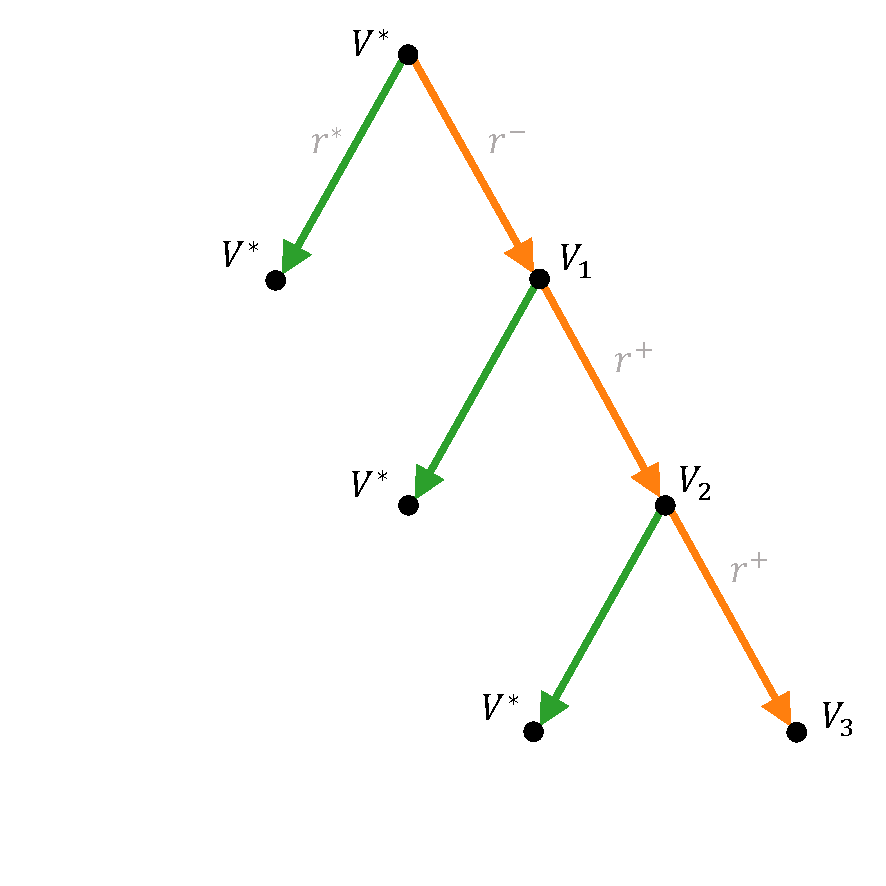
\includegraphics[trim={3.5cm 2cm 0.5cm 0.5cm}, clip, width=0.5\linewidth]{img/gbop/mdp_tree.pdf}
    \caption{Planning tree of the \gls{MDP} $\cM$ of \Cref{fig:mdp}}.
    \label{fig:mdp-tree}
\end{figure}
\begin{lemma}
 Any sequence of actions in $A\setminus{a_1}$ is in $\Tau^\infty$.
\end{lemma}
\begin{proof}
Any such sequence of actions yields the sequence of rewards $r^-, r^+, \dots,r^+$. and end up in the state $s^+$ with value at least $V^\star$ (obtained by further taking $a_1$ indefinitely). Thus its value $V_h$ verifies, 
\begin{align*}
    V_h &\geq \sum_{t=0}^{h-1} \gamma^t r_t + \gamma^h V^\star\\
    &= r^- - r^+ + \sum_{t=0}^{h-1} \gamma^t r^+ + \gamma^h V^\star \\
    &= (-\frac{\gamma}{1-\gamma} - 1)S + \frac{1-\gamma^h}{1-\gamma} (r^\star + S) + \gamma^h V^\star\\
    &= V^\star - S\frac{\gamma^h}{1-\gamma} \geq V^\star - \frac{\gamma^h}{1-\gamma}
\end{align*}
\end{proof}

We can directly conclude that $\kappa \geq \limsup{|\{a_2,\dots,a_K\}^h|^{1/h}} = K-1$.

Now, consider the nodes expanded by \GBOPD. The first expansion is that of the root, which discovers $s^\star$ and $s^+$. In the absence of information on these two state, the bound $V_{\max}$ is used and the first action $a_1$ gets a higher $\overline{U}$ that any other action $a_2,\dots,a_K$ since $r^\star \geq r^-$. Hence, at the second iteration, the node $a_1$ gets expanded. At this point, the self-loop of the state $s^\star$ is discovered, which means that form now on the bounds verify $L_n(a_1) = V^\star = U_n(a_1)$ for $n\geq2$, which means that $L_n(a_1\cA^*)-U_n(a_1\cA^*) = 0$. The nodes $a_2,\dots,a_K$ can be expanded at most once before the entire \gls{MDP} is discovered and $L_n=V=U_n$ over the entire tree, which means that $\Tau_n^\infty$ is the set of optimal nodes, i.e. the nodes in the only optimal sequence $a_1^\star$. Hence, $\kappa_\infty = 1.$ 
\end{subappendices}
